\documentclass[a4paper,12pt]{article} 	
\usepackage[legalpaper, portrait, margin=1in]{geometry}

% class, page size, fontsize 
\usepackage{setspace}
\usepackage[english]{babel}
\usepackage{layouts}
\usepackage{soul, color}
\usepackage{amsmath} 							% math fonts
\usepackage{amsfonts}
\usepackage{amssymb}
\usepackage{mathtools}
\usepackage[mathscr]{euscript}
\usepackage{hyperref}
\hypersetup{colorlinks = true, linkcolor = red, citecolor = blue} 
\usepackage{cleveref}
\usepackage{graphicx}
\usepackage[font=small,labelfont=bf]{caption}
\usepackage[T1]{fontenc}
\usepackage{authblk}							% author block
\usepackage[utf8]{inputenc}
\usepackage{csquotes}
\usepackage[round]{natbib}						% BibTex Layout
%\usepackage{appendix}		% Appendix
\usepackage{caption}
\usepackage{url}
\usepackage{hyperref}
\usepackage{algorithm,algcompatible,amsmath}	% algorithm package
\algnewcommand\INPUT{\item[\textbf{Input:}]}	% algorithm command declaration
\algnewcommand\OUTPUT{\item[\textbf{Output:}]}	% algorithm command declaration
%\usepackage{lineno}
%\linenumbers
%\graphicspath{{/Users/Rasmus/Dropbox/pivotal/pv_analyses/}}
%\usepackage{multirow}
%\usepackage{multibib} % for splitting references between main text and supplementary material
%\newcites{SM}{SM References} % for referencing supplementary
\DeclareUnicodeCharacter{2060}{\nolinebreak}

%%%%%%%%%% START DOCUMENT

\title{Prediction Error and Episodic Memory - Insights from Computational Models}

\author[1]{Francesco Pupillo}
\author[1]{Javier Ortiz-Tudela}
\author[2]{Rasmus Bruckner}
\author[1]{Yee Lee Shing}
\affil[1]{Goethe-Universität Frankfurt}
\affil[2]{Freie Universität Berlin}
\date{November 2021}

\begin{document}
{
\hypersetup{linkcolor=black}
\tableofcontents
}
\setlength{\parindent}{10ex}
%\newgeometry{a4paper, top=25mm, left=25mm, right=25mm,bottom=30mm,
%headsep=10mm, footskip=12mm}

\maketitle

\noindent
Raw data and scripts used for this project is available on GitHub. \url{https://github.com/FPupillo/PreM-Computational} 

\doublespacing

\begin{abstract}
\noindent
Predictive processing accounts propose that our brain constantly tries to match top-down internal representations with bottom-up incoming information from the environment. Predictions of varying degrees can lead to corresponding prediction errors depending on whether or not the information encountered in the environment conforms with prior expectations. Theoretical and computational models assume that prediction error has significant, beneficial effects on learning and memory. While there is strong evidence on the effects of prediction error on learning, relatively less evidence is available regarding its effects on memory. Previous studies on the effects of prediction error on memory using computational models have manipulated the amount of reward participants received on probabilistic learning task and showed contrasting evidence. We decided to use a more naturalistic task in which the reward is not explicitly manipulated but learned from the correct or incorrect outcome of the predictions . Participants first formed expectations of different strengths for context/object-category associations in a contingency-learning paradigm. In the encoding phase that followed, they were asked to predict the expected category of the objects after being cued by specific contexts. The objects that were then shown could either match or violate their previously learned expectations. Finally, participants were asked to complete a surprise recognition test. We used a reinforcement learning model to derive subject-specific trial-to-trial estimates of prediction error. In two different experiments, results showed that prediction error at encoding influenced subsequent memory as a function of the outcome of participants’ predictions (correct vs incorrect). Precisely, when participants correctly predicted the object category, stronger prediction error (as an outcome of weak prior) led to enhanced memory. In contrast, when participants incorrectly predicted the object category, stronger prediction error (as an outcome of strong prior) led to impaired memory. These results reveal a computationally specific influence of prediction error on memory formation, highlighting the important moderating role of prediction accuracy.     
\end{abstract}

%%%%%%%%%% INTRODUCTION

In our daily interaction with the environment we are confronted with a great amount of information which cannot be all processed in detail, given the limited resources of our cognitive systems. In order to simplify the complexity of the world, our brain tries to extract the regularities in order to be able to react to environmental demands in efficient ways. One way of extracting regularities from experience is to rely on repetitions and associations of events, which lead to the creation of increasingly complex knowledge \citep{Ghosh2014, Tse2007}. This accumulation of knowledge across similar experiences that can subsequently form expectations and orient our actions is what characterizes reinforcement learning \citep{Sutton1998}. In reinforcement learning, individuals incrementally learn, over experiences, to form expectations in order to successfully predict future events. As an example from real life, we may learn after several experiences that book stores specialize on different genres, such as crime or romance. Learning this association will guide us to go to a precise book store if we are looking for that particular book. \par 
Events can, however, sometimes deviate from our expectations. We may go to a book store we have learnt being specialized in crime books and discover that the crime book we are looking for is not there. We might then decide to go to another book store, which we know has equal coverage of different genres. Despite our low expectations, we may find the crime book we were looking for in the generalist book store. In such situations, the difference between expectations and the experienced event generates a prediction error (PE) signal which may change expectations and future decisions. PE is crucial in promoting learning by driving the updating of prior knowledge \citep{Ergo2020, Friston2018}. In reinforcement learning models, the learning rate regulates the extend to which the current prediction error is used to update the expectations \citep{Sutton2018a}. A larger learning rate results in increased update of the expectations, shifting the expectations towards the most recent outcomes. On the contrary, smaller learning rate shifts the expectations towards older estimates. Another key aspect that may modulate the effect of PE on updating is the outcome of the predictions. In fact, correctly predicting an event generally results in an increase in the strength of the expectations that led to the prediction, whereas incorrectly predicting leads to a weakening of the related expectations  \citep{Daw2013}. %(REFERENCE? For example Kim et al. 2014 paper from Turk-Browne's lab)
For example, correctly predicting that the book we are looking for is in a specific book store will increase our belief that we need to go to that store to find the brand. Conversely, when we do not find the book in the store our belief will not be as strong as before. Prediction outcome also affects differently the amount of update that follows a PE, as individuals tend to update their belief more as a consequence of positive outcomes compared to negative ones \citep{Lefebvre2017, sharot2007neural, sharot2011unrealistic, sharot2016forming}.  \par
In addition incremental learning, individuals are also capable of encoding distinct, temporally specific episodic memories of events. For example, remembering the precise occasion in which the desired book was found in a distinct store. 
While there is a a great amount of evidence on the effects of PE, learning rate, and prediction outcome on incremental learning, its  effects on the formation of new memories are still not fully understood.\par

%According to theoretical and computational accounts, events that violate prior expectations would improve memory encoding by promoting the formation of  distinct memory traces \citep{McClelland1995a, VanKesteren2012}. However, studies investigating the interplay between memory encoding and PE show contrasting results. In fact, some studies have found that information that is congruent with prior knowledge tends to be better remembered than incongruent one \citep{Bein2015,BrodGarvinShingYee2019}⁠, while other studies have found that incongruent events may be better remembered than congruent ones \citep{Greve2017,Kafkas2018}.\par
The study of the relationship between prior expectations and learning has benefited from the use of computational models. Reinforcement learning models in particular has been used, due to their ability to confer a precise mechanistic role to PE in learning and map it to its neural substrates. In fact, it has been shown that firing patterns of mesencephalic dopamine neurons and also Blood-Oxygen-Level Dependent (BOLD) signal in the striatum resemble the PE signal used in reinforcement learning models \citep{Daw2011, McClure2003, Schultz1997}. This dopaminergic-dependent PE is thought to inform future predictions by indicating deviations between observed and predicted outcomes \citep{Daw2013, Niv2008, Rangel2008a, Rushworth2008}, thus encouraging the repetition of actions that are better than expected (positive PE) and discouraging the repetition of actions that are worse than expected (negative PE, \citealp{Schultz2016, Steinberg2013}). An emerging line of research examines the relation between prediction errors and long term memory formation as a potential mechanism that explains interactions between memory and learning. These studies are motivated by both anatomical considerations that the hippocampus receives dopaminergic input (e.g., \citealp{Lisman2005}) and functional findings on interactions between hippocampus and striatum (e.g., \citealp{Poldrack2001}). \par
Several studies have manipulated the amount of the reward participants expected and received, linking the obtained reward PE experienced at the time of item presentation or immediately after presentation to the subsequent recognition of those items \citep{Rouhani2018,Rouhani2021, Jang2019, de2018signed}. Some studies have found improved memory for surprising outcomes, namely better memory for items associated to both better- and worse-than-expected outcomes \citep{Rouhani2018, Rouhani2021}.
By contrast, some other studies found that better-than-expected outcomes, compared to worse-than-expected ones, led to improved later recognition  \cite[][Experiment 2 ]{Jang2019, de2018signed, Rouhani2021}. The present study manipulated expectations to create PE of different strength and related it to the strength of the encoding. %⁠ Therefore, also when considering reward PE, results are divided among effects due to signed PE, in which there is a contrast between the positive and negative valence of PE, and effects related to unsigned prediction error, in which the unexpectedness of the events, independently of the valence, influences memory encoding. Interestingly, studies finding memory benefits for all surprising events (both better- and worse-than-expected) used a passive Pavlovian paradigm, with outcome being independent of participants' choice. Conversely, studies finding a positive, linear relationship between signed PE and encoding used active learning paradigms in which participants received outcomes related to their choices, suggesting a modulating role of the valence of PE. \citep{Rouhani2018, Rouhani2021}.\par
The aforementioned studies using computational models manipulated expectations by using rewards. Since in everyday life learning does not occur always in the presence of explicit rewards, it is crucial to consider the mechanistic effects of PE \textit{per se}, in contexts in which no explicit information about the reward is conveyed. A different way of looking at the relationship between expectations and memory may involve generating them through associations between a context (e.g., going to a grocery store to look for a brand) triggering some expectations (e.g., more or less strong belief about the presence of the brand). and a matched or unmatched outcome (e.g.,finding or not finding the expected brand). 
In addition, the studies cited above have looked at the effects of PE in conditions in which participants were actively learning novel associations. However, familiar situations in which the environmental structure has been learned and contingencies are no longer novel are more common in real life. \par
We therefore designed a task in which participants learned probabilistic associations between contexts and object categories. After a learning phase in which the expectations were established, participants were presented with the contexts and had to predict the category of trial-unique objects that appeared at the end of each trial. In order to generate different levels of PE strength, we quantified expectations by using gradually different contingencies. The probability of a certain category following a context was systematically manipulated so that for some contexts expectations were stronger than for others.
Findings using the same data as the current study reported in a separate publication \citep{ortiz2021not} showed that such context manipulation affected recognition memory. Specifically, results showed that memory was better for contexts with weaker expectations. In the present study, we use participants' behaviour in the encoding phase and parameters derived by model fitting to perform additional analyses. We used a reinforcement learning model to derive learning rates and trial-level PE experienced during the presentation of the images and relate them to the likelihood of subsequently recognizing the items in a following surprise recognition test. The computationally derived PE reflected how unexpected the presentation of an object category in a given context was to participants. The procedure thus allowed to test whether episodic memory for the objects was related to learning rate and PE experienced in situations where no explicit reward was provided.
\par
 We reasoned that if increased learning rate results in higher weights on more recent events \citep{Daw2013}, it should also bias the system towards increased encoding, resulting in better episodic memory. In relation to PE, we hypothesised that if unpredicted events \textit{per se} improve memory encoding, we would observe a positive relationship between PE and memory encoding, so that memory performance would be better for the more unpredicted events. Contrarily, if the effect of PE on memory is modulated on whether or not the prediction was correct, we would observe an interaction between PE and choice outcome so that PE improves memory for better than expected outcomes, while impairs memory for worse than expected outcomes. In a series of two experiments, we showed that the likelihood of correctly recognizing an item scaled with PE and was modulated by prediction outcome at encoding. Specifically, when participants correctly predicted the object category stronger PE led to improved memory encoding, whereas for incorrect predictions stronger PE led to impaired encoding. %This pattern was replicated in a second experiment, in which the contingencies of the context/object-category pairs were more graded.



\section{Results}
In both experiments, participants performed a task in which they were asked to predict the category of trial-unique objects that would follow a specific context. Instructions were given to indicate that each context was predictive of one object category, but there was no indication about which category and with which contingency (see Figure \ref{fig:Methods}). Participants learned the associations between contexts and object categories during a learning phase (phase 1), in which they received feedback on every trial. In a subsequent phase (phase 2), a new set of never-seen-before objects (but belonging to the same object categories as the ones in phase 1) was introduced and participants were asked to continue doing the same task as in the previous phase. Importantly, participants no longer received explicit feedback on their performance. Finally, they completed a recognition memory test, where they were asked to recognize the objects presented in phase 2 among several distractors.
%Some findings of these data are reported in a separate publication \citep{ortiz2021not}. However, we performed additional analyses for different purposes that are reported here.

\begin{figure}[ht!]
\centerline
{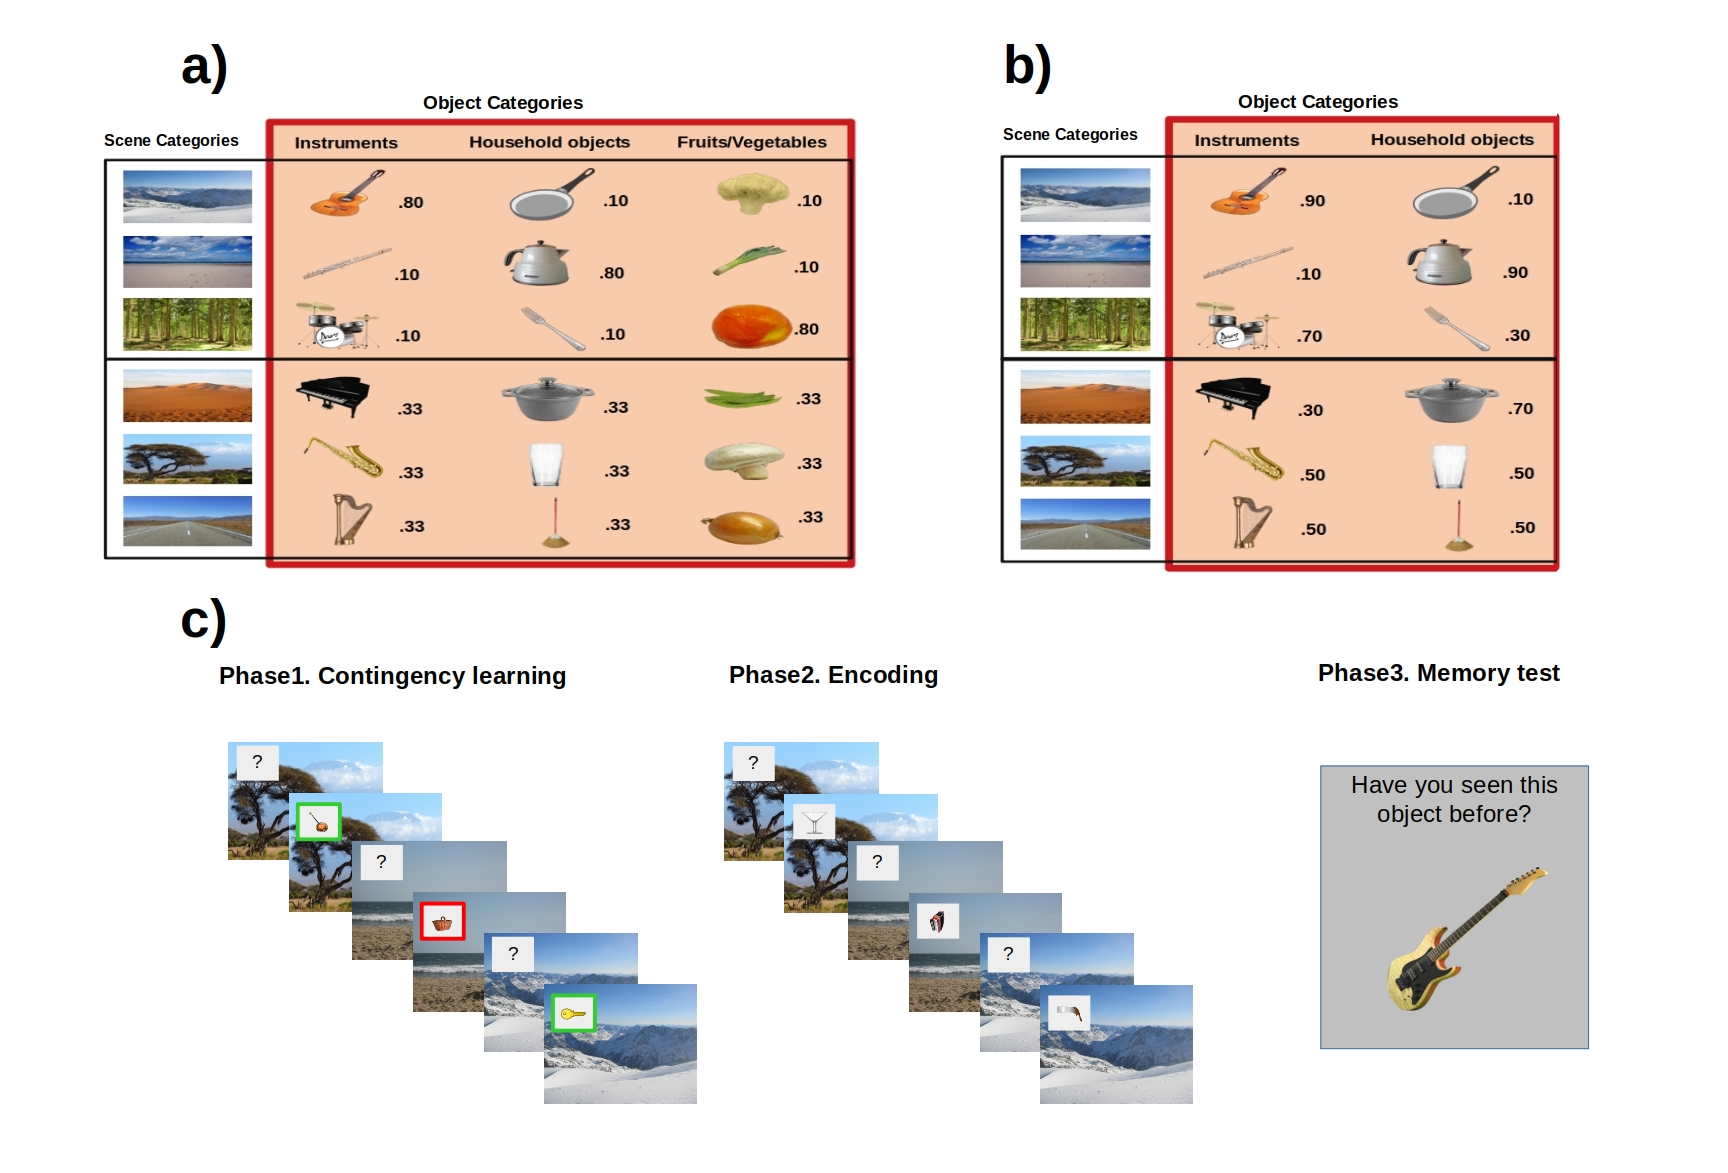
\includegraphics[width=1.3\textwidth]{figures/methods.All.jpg}}
\caption{\textbf{Illustration of the Methods.} Illustration of the scene/object-category contingencies  for a) Experiment 1 and b) Experiment 2. Note that each object is representative of its object category and that different items from each category where used for each cell shown here. c), illustration of the three phases of the study. }
\label{fig:Methods}
\end{figure}


In Experiment 1, participants were presented with six contexts. Each of the contexts was predictive of the object categories following specific contingencies (Figure \ref{fig:Methods}.1):in half of the contexts, the three objects categories was presented 80 \% of the times, and the remaining two object-categories 10 \% of the times; in the other half of the contexts, all the three object categories were equally likely. In experiment 2, two instead of three object categories were used. In addition, the contingencies were kept 90-10, 50-50, and 70-30, respectively. This manipulation allowed to sample more points along the PE continuum. To reach the desired contingencies for each condition, filler objects from the same object categories were introduced and repeated several times, increasing the number of the trials especially in the strong prior conditions. Recognition memory for these objects was not tested.

\subsection{Learning Performance}
In both experiment 1 and experiment 2, learning performance during the contingency learning and encoding phases showed that participants understood the task correctly and were able to learn to predict the object category that was more likely to be presented for each context. Participants’ cumulative accuracy tended to approximate true probability for each context and experiment, as shown in Figure \ref{fig:participantsLer}.



\begin{figure}[ht!]
\centerline
{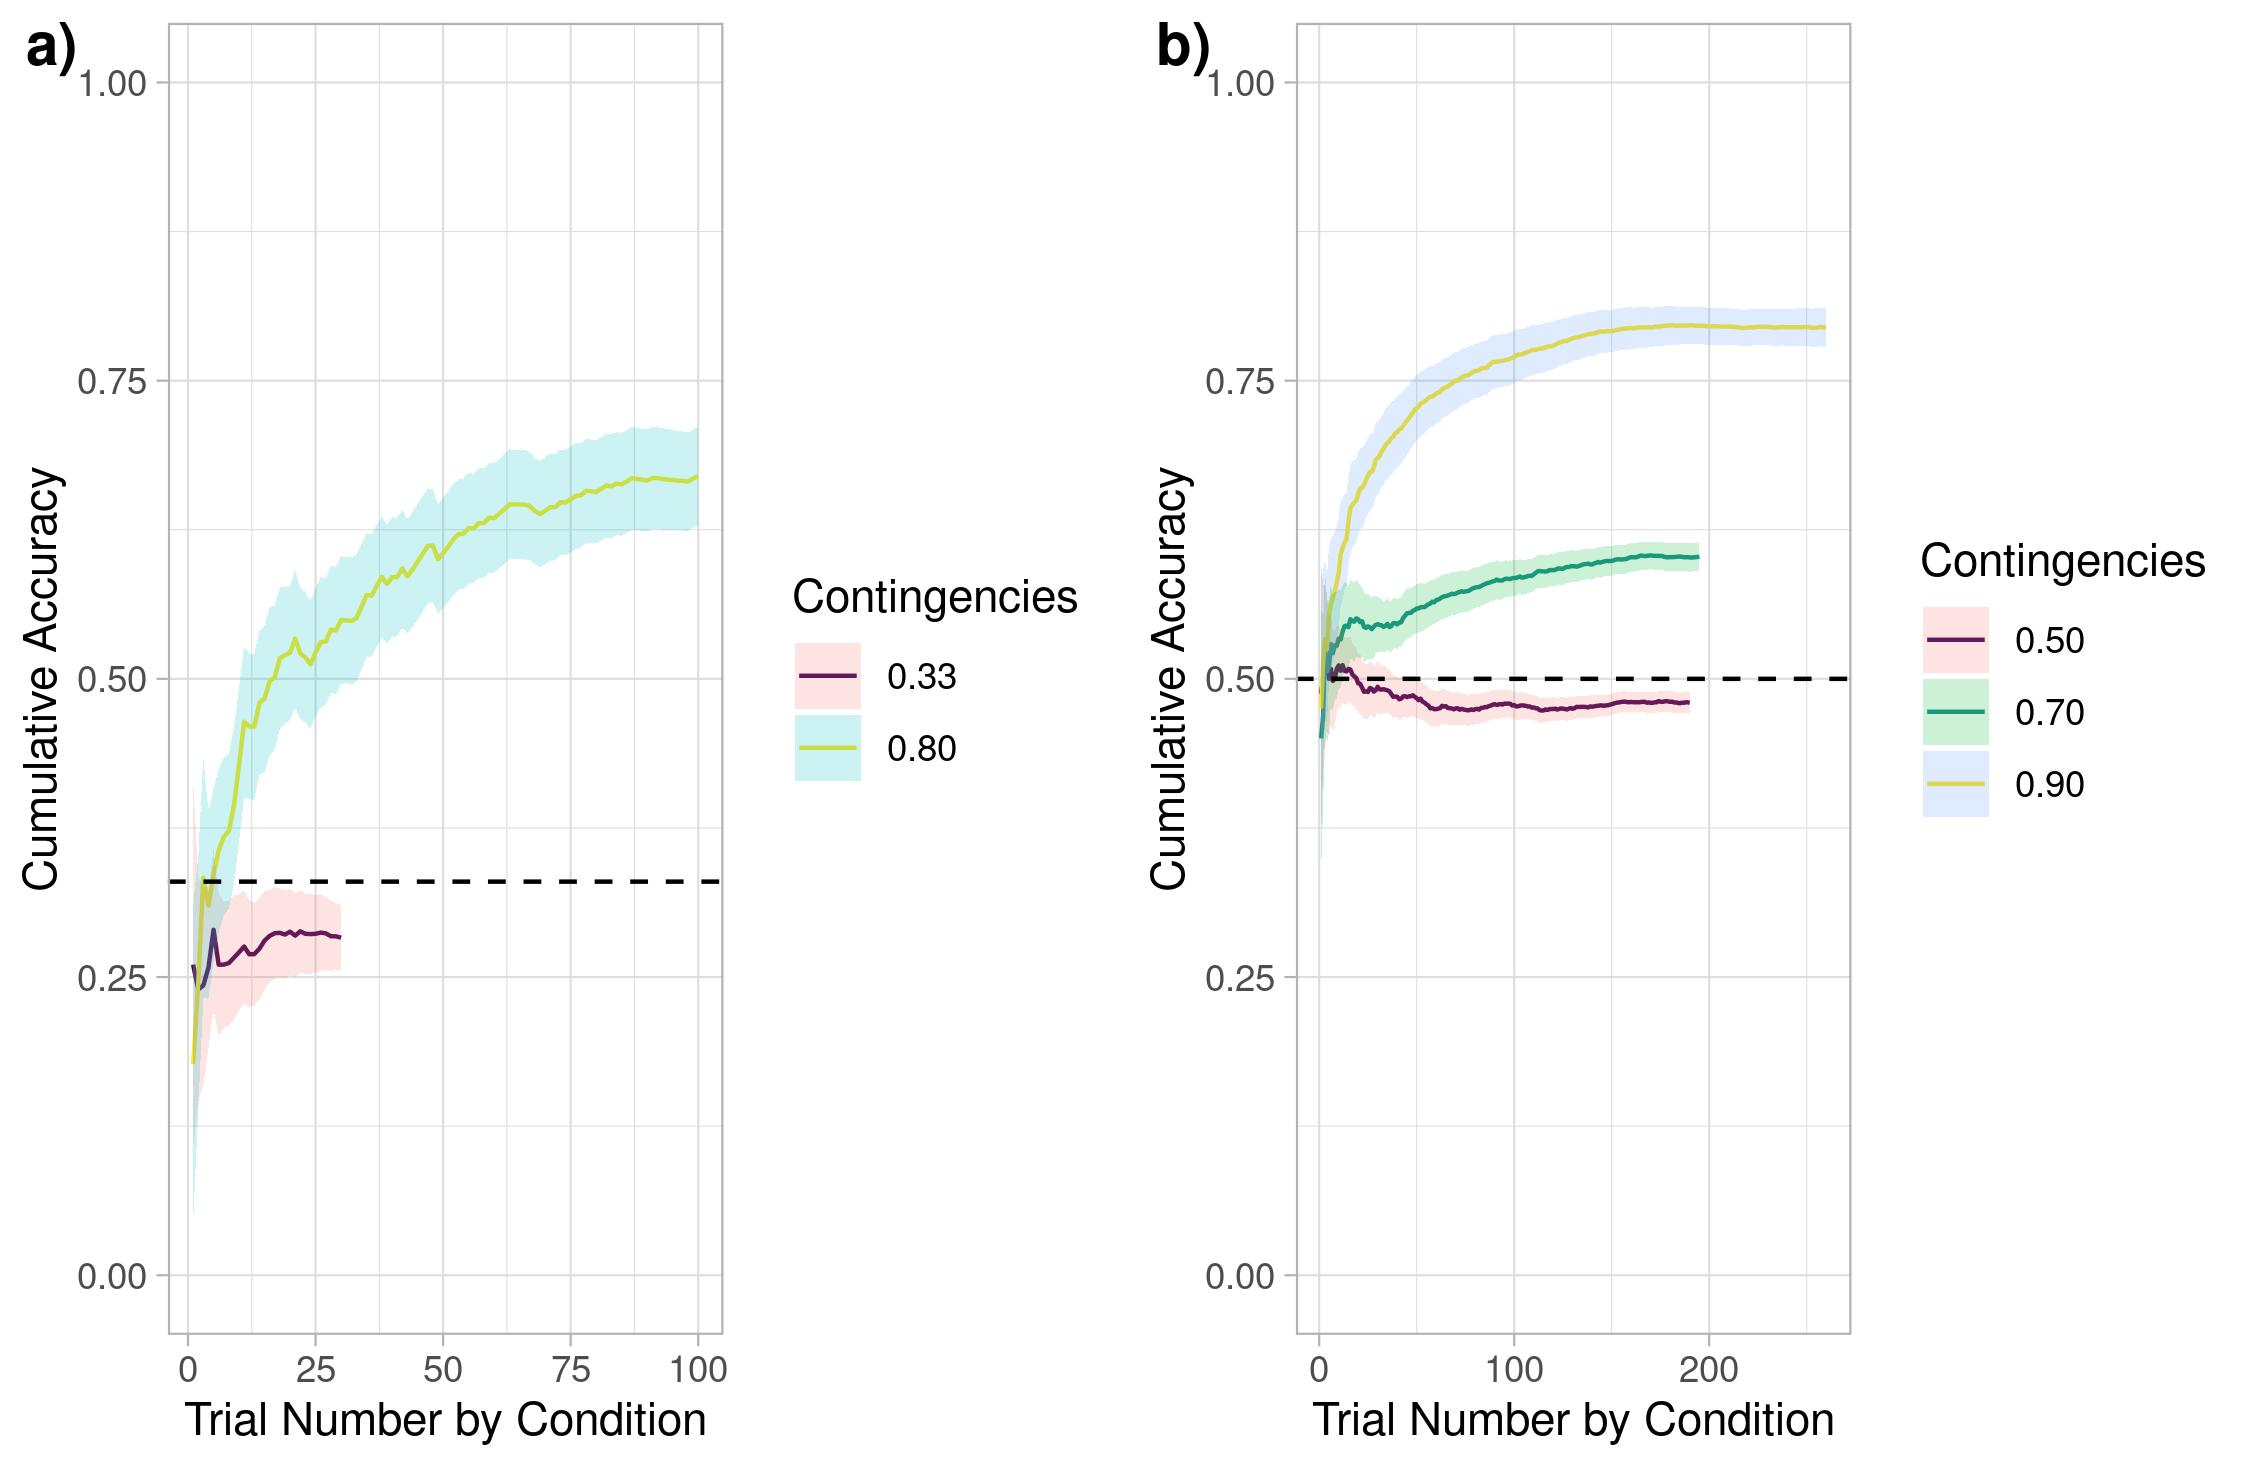
\includegraphics[width=1\textwidth]{figures/cumAccbySceneAll.jpg}}
\caption{\textbf{Participants' learning performance.} Participants' learning performance at the learning and encoding phase for a) experiment 1 and b) experiment 2. Trial number by contingency is represented in the x axes, while cumulative accuracy is shown on the y axes. The different colours represent the scene conditions.The dashed line represents chance level while shadows represent standard error.}
\label{fig:participantsLer}
\end{figure}




\subsection{Computational Models}
In order to derive trial-level PE at contingency learning and encoding phases, variants of reinforcement learning model \citep{Sutton2018a} were fitted to the behavioural data. We fit the reinforcement learning models to data from both learning and encoding phase pooled together. The use of reinforcement learning models allowed to capture the process of establishing prior expectations while learning the object-category contingencies for the different contexts. In the reinforcement learning models, an agent is assume to learn values of context-category associations by adding the current expected value to a learning rate $\alpha$ multiplied by the PE. The learning rate $\alpha$ is a value between 0 and 1 that determines the influence of the current prediction error on the expected values. It represents the extent to which evidence from the current trial is used to update the expectations: Higher learning rate weights more the present evidence and the extend to which it deviates from the value estimates, while lower learning rate weights more the estimated values, and thus the past trials.  We fitted three different reinforcement learning models that made different assumptions on how participants learned the context/object-category associations (see Methods): (1) an instructive model with a learning rate (fixed across participants) that decreases across trials (dLRI), and updates the expected values by increasing the value of the object category presented on a given trial and decreasing the values of the categories not presented, regardless of the choices made by the participants; (2) an instructive model with a decreasing learning rate  $\alpha$ that was free to vary between individuals; (3) an instructive model with a free constant learning rate $\alpha$ (fLRI); (4) an evaluative model with a free constant learning rate (fLRE), where the expected values were updated depending on the accuracy of participants' actions, increasing for correct predictions and decreasing for incorrect ones. \par
The dLRI considers how the expected values should be updated optimally, since it is derived from a Bayesian formulation of the task (see Methods and Supplemental Material). In this optimal Bayesian formulation of learning, prediction error is assumed to have its maximal influence on learning in the early trials, and decreases as a function of the inverse of the number of the trials. In this model, the only parameter that was estimated was the 'inverse temperature' $\beta$, which regulates the stochasticity/determinism trade-off in selecting the action depending on the expected values: Higher values of $\beta$ represent more probable preference of the higher context/object-category associations, while lower values also consider low-strength associations, producing more noisy choices. 
In addition to the $\beta$ parameter, the instructive model with the free decreasing learning rate estimates a learning rate $\alpha$ that was free to vary across individuals and decreased inversely proportional to the number of the trials. The instructive fLRI and evaluative fLRE models estimated a learning rate $\alpha$ that was constant throughout the learning and encoding phases, and free to vary across individuals in order to capture participants' distinct learning rates. These models make different assumptions on how participants used information to update the expected values. In fact, while evaluative free-learning rate model (fLRE) assumes that participants use the feedback received (correct vs incorrect) to update only the category chosen, the instructive free-learning rate model (fLRI) implies that on each trial participants update all the associations by strengthening the one between the context and the category presented, while lowering the associations with that context and the categories that were not presented at that trial.  \par
Prior to fitting the models to participants' data, we ensured that the models could distinguish among different parameters' value and also generate qualitatively different data (see 'Parameter Recovery' and 'Model Recovery' in Methods and Supplemental Material). Then, the three models were fit to participant's data, and the parameters of best fit were estimated as the parameters that maximized the likelihood of participants' choices. 

\subsubsection{Model Comparison}
In addition to calculating log-likelihood, we calculated the Bayesian information criterion (BIC) for each model and for each subject, by multiplying the maximum likelihood (i.e. the likelihood for the parameters of best fit) by the number of free parameters in the model. This approach penalizes models with more parameters. We then marked the number of participants for which each model was the best fit, as well as the evidence for it, computed as the BIC difference between the best and the second best model. Results are shown in Figure \ref{fig:ModelComparison}. Table \ref{tab:ModelComp} show BIC values and the the number of participants for which a model was the best fit, as well as the number of participants for which there was strong evidence, for both Experiment 1 and Experiment 2. 


\begin{figure}[ht!]
\centerline
{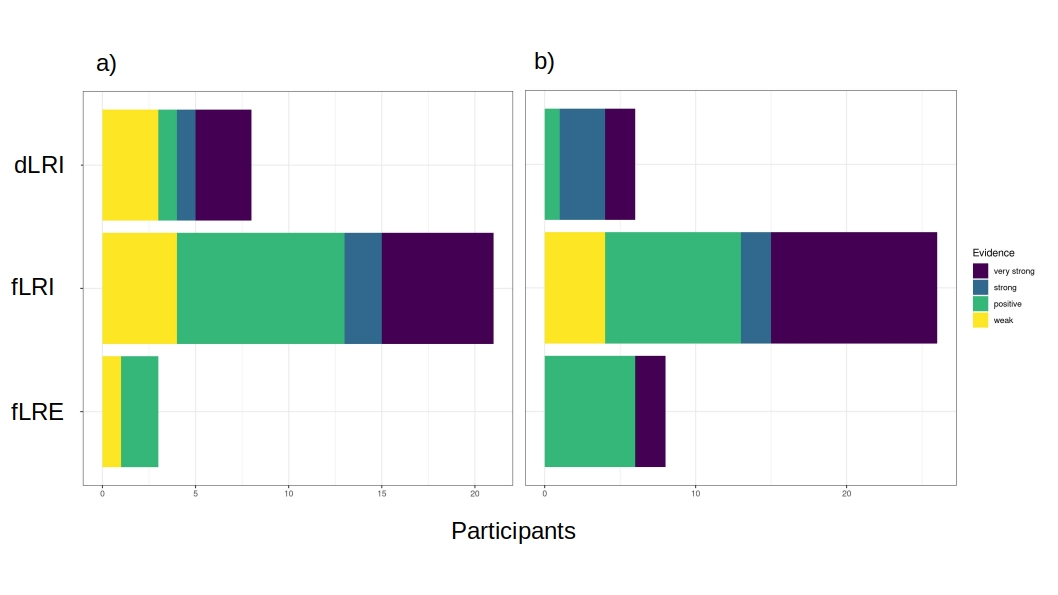
\includegraphics[width=1\textwidth]{figures/ModelComparisonAll.jpg}}
\caption{\textbf{Model Comparison.} Results of model comparison for a) experiment 1 and b) experiment 2. Evidence for the best model for each participants is shown.}
\label{fig:ModelComparison}
\end{figure}

\begin{table} 
    \centering 
    \caption{\label{tab:ModelComp}Model Comparison. BIC values and standard errors for each model for Experiment 1 and experiment 2. \textit{Best(N)} and \textit{Very strong(N)} refer to the number of participants for which the model was the best fit and for which there was very strong evidence, respectively   }
    \scalebox{1}{
    \begin{tabular}{l l l l}

     \hline

   Model/Experiment & BIC (\textit{se}) & Best(N) & Very Strong (N) \\
     \hline
    \textbf{Experiment 1} \\ 

  dLRI & 289.3(2.5) & 2 & 1 \\
  dfLRI & 277.0(2.0) & 2 & 0 \\
  fLRI & 266.4(1.7) & 20 & 6 \\
  fLRE & 271.4(2.7) & 8 & 3 \\

         \textbf{Experiment 2} \\
  dLRI & 801.2(4.3) & 5 & 2 \\
  dfLRI & 793.1(2.9) & 7 & 3 \\
  fLRI & 783.1(3.7) & 23 & 9 \\
  fLRE & 774.3(2.9) & 5 & 2 \\
     \hline

    \end{tabular}
}
    \end{table}

Model comparison established that the instructive model with the free learning rate (fLRI) explained participants behaviour better than the other models. In fact, the overall BIC was smaller (indicating better fit), and the number of participants for which it was the best model were 20 over a total of 32 participants for experiment 1, and 23 over a total of 40 participants for experiment 2. In addition, there was very strong evidence for it being the best model for 6 participants in experiment 1 and 9 participants in experiment 2. %Therefore, the best fitting model was the model that considers instructive feedback and estimates a specific learning rates for each participant. 
These results indicate that participants learning processes deviate from the behaviour of an optimal Bayesian observer and that are best described by using individual learning rates. In addition, model comparison show that most participants used the category information of the object presented at the end of each trial to update all the context/object-category associations, and not only the associations related to the chosen object category.

\subsubsection{Model Validation}
We then validated the winning model by looking at the ability of the model to generate performance which was qualitatively similar to participants' actual behaviour. For each actual participant, we simulated data on the learning and encoding tasks using the best fitting model (fLRI) and its estimation of best fitting parameters. The model simulations included the actual task structure. In order to evaluate model's simulations, we calculated cumulative accuracy for the data generated by the model and compared it to participants' actual cumulative accuracy. Figure \ref{fig:simvsemp_Exp1} and Figure \ref{fig:simvsemp_Exp2} show that the simulated models capture participants' behaviour. Data simulated from the dLRI and the fLRI models can be found in the Supplemental Material (Figure \ref{fig:simvsemp_dlr_flrI_exp1} and Figure \ref{fig:simvsemp_dlr_flrI_exp1})



\begin{figure}[ht!]
\centerline
{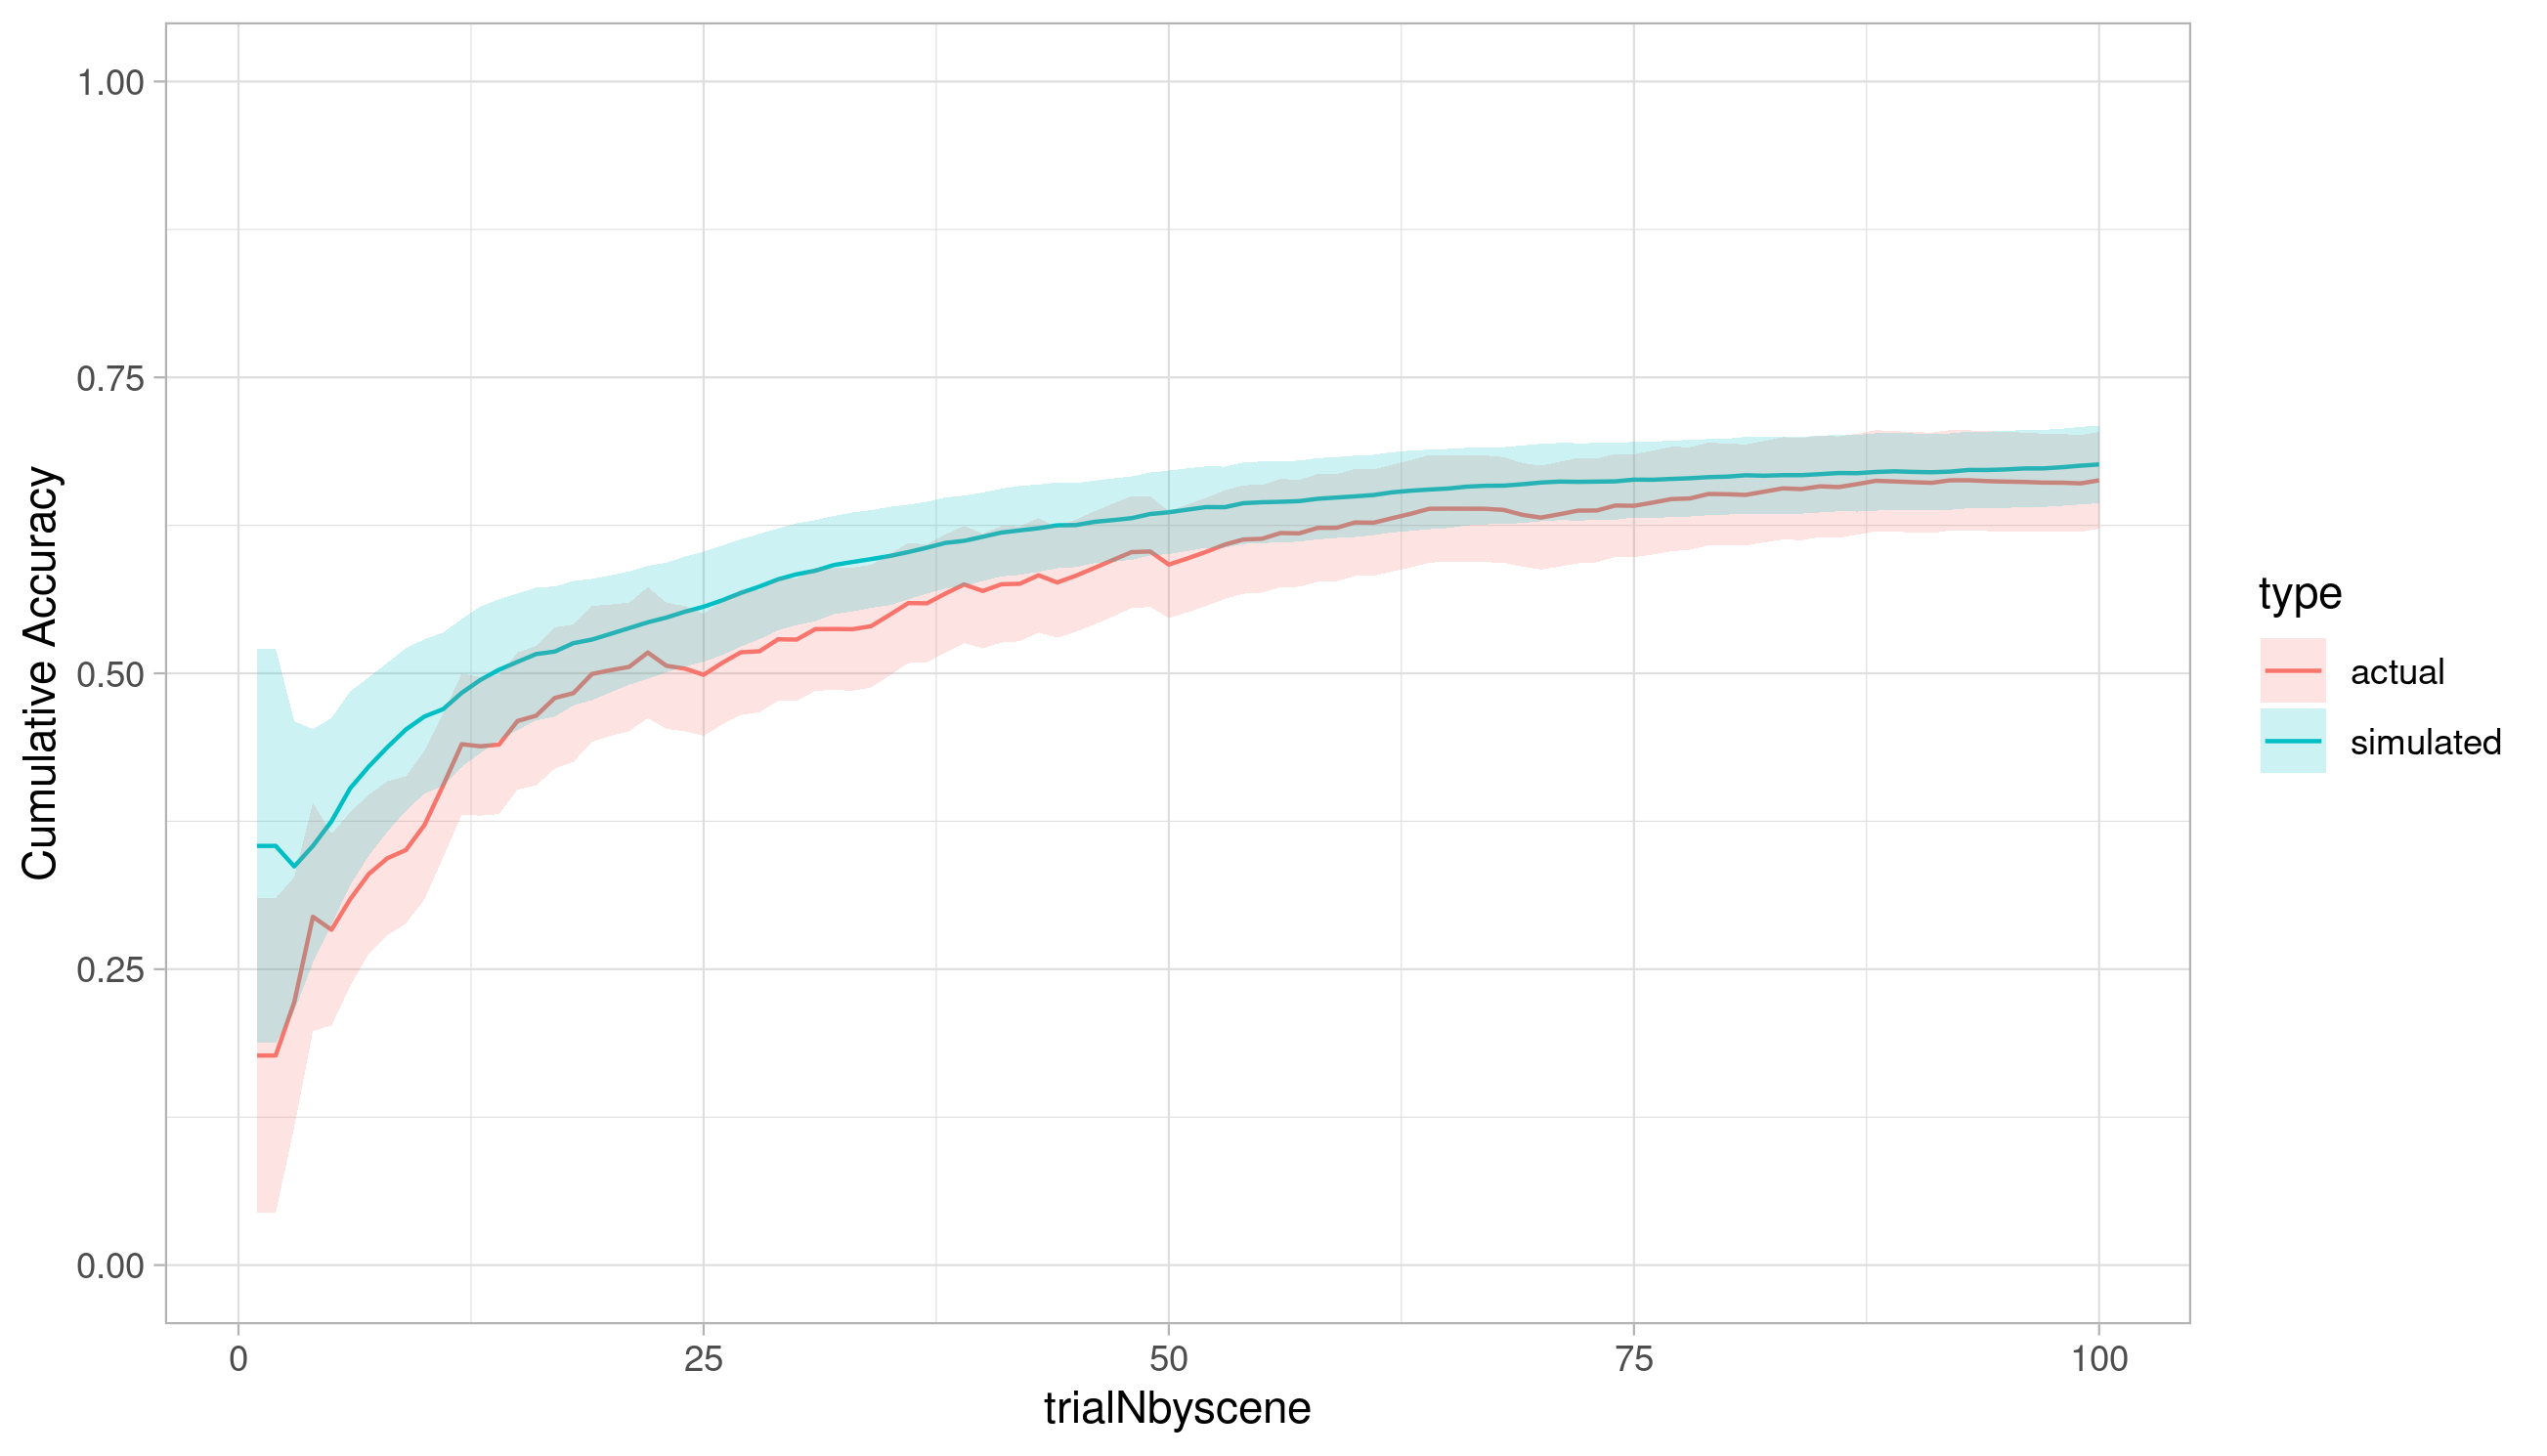
\includegraphics[width=1\textwidth]{figures/SimulatedVsActual.exp=exp1.mod=fLR_Instr.png}}
\caption{\textbf{Simulated vs Empirical Data - Experiment 1.} Simulated data (red line) and actual data (green line) overlapped, for experiment 1.}
\label{fig:simvsemp_Exp1}
\end{figure}

\begin{figure}[ht!]
\centerline
{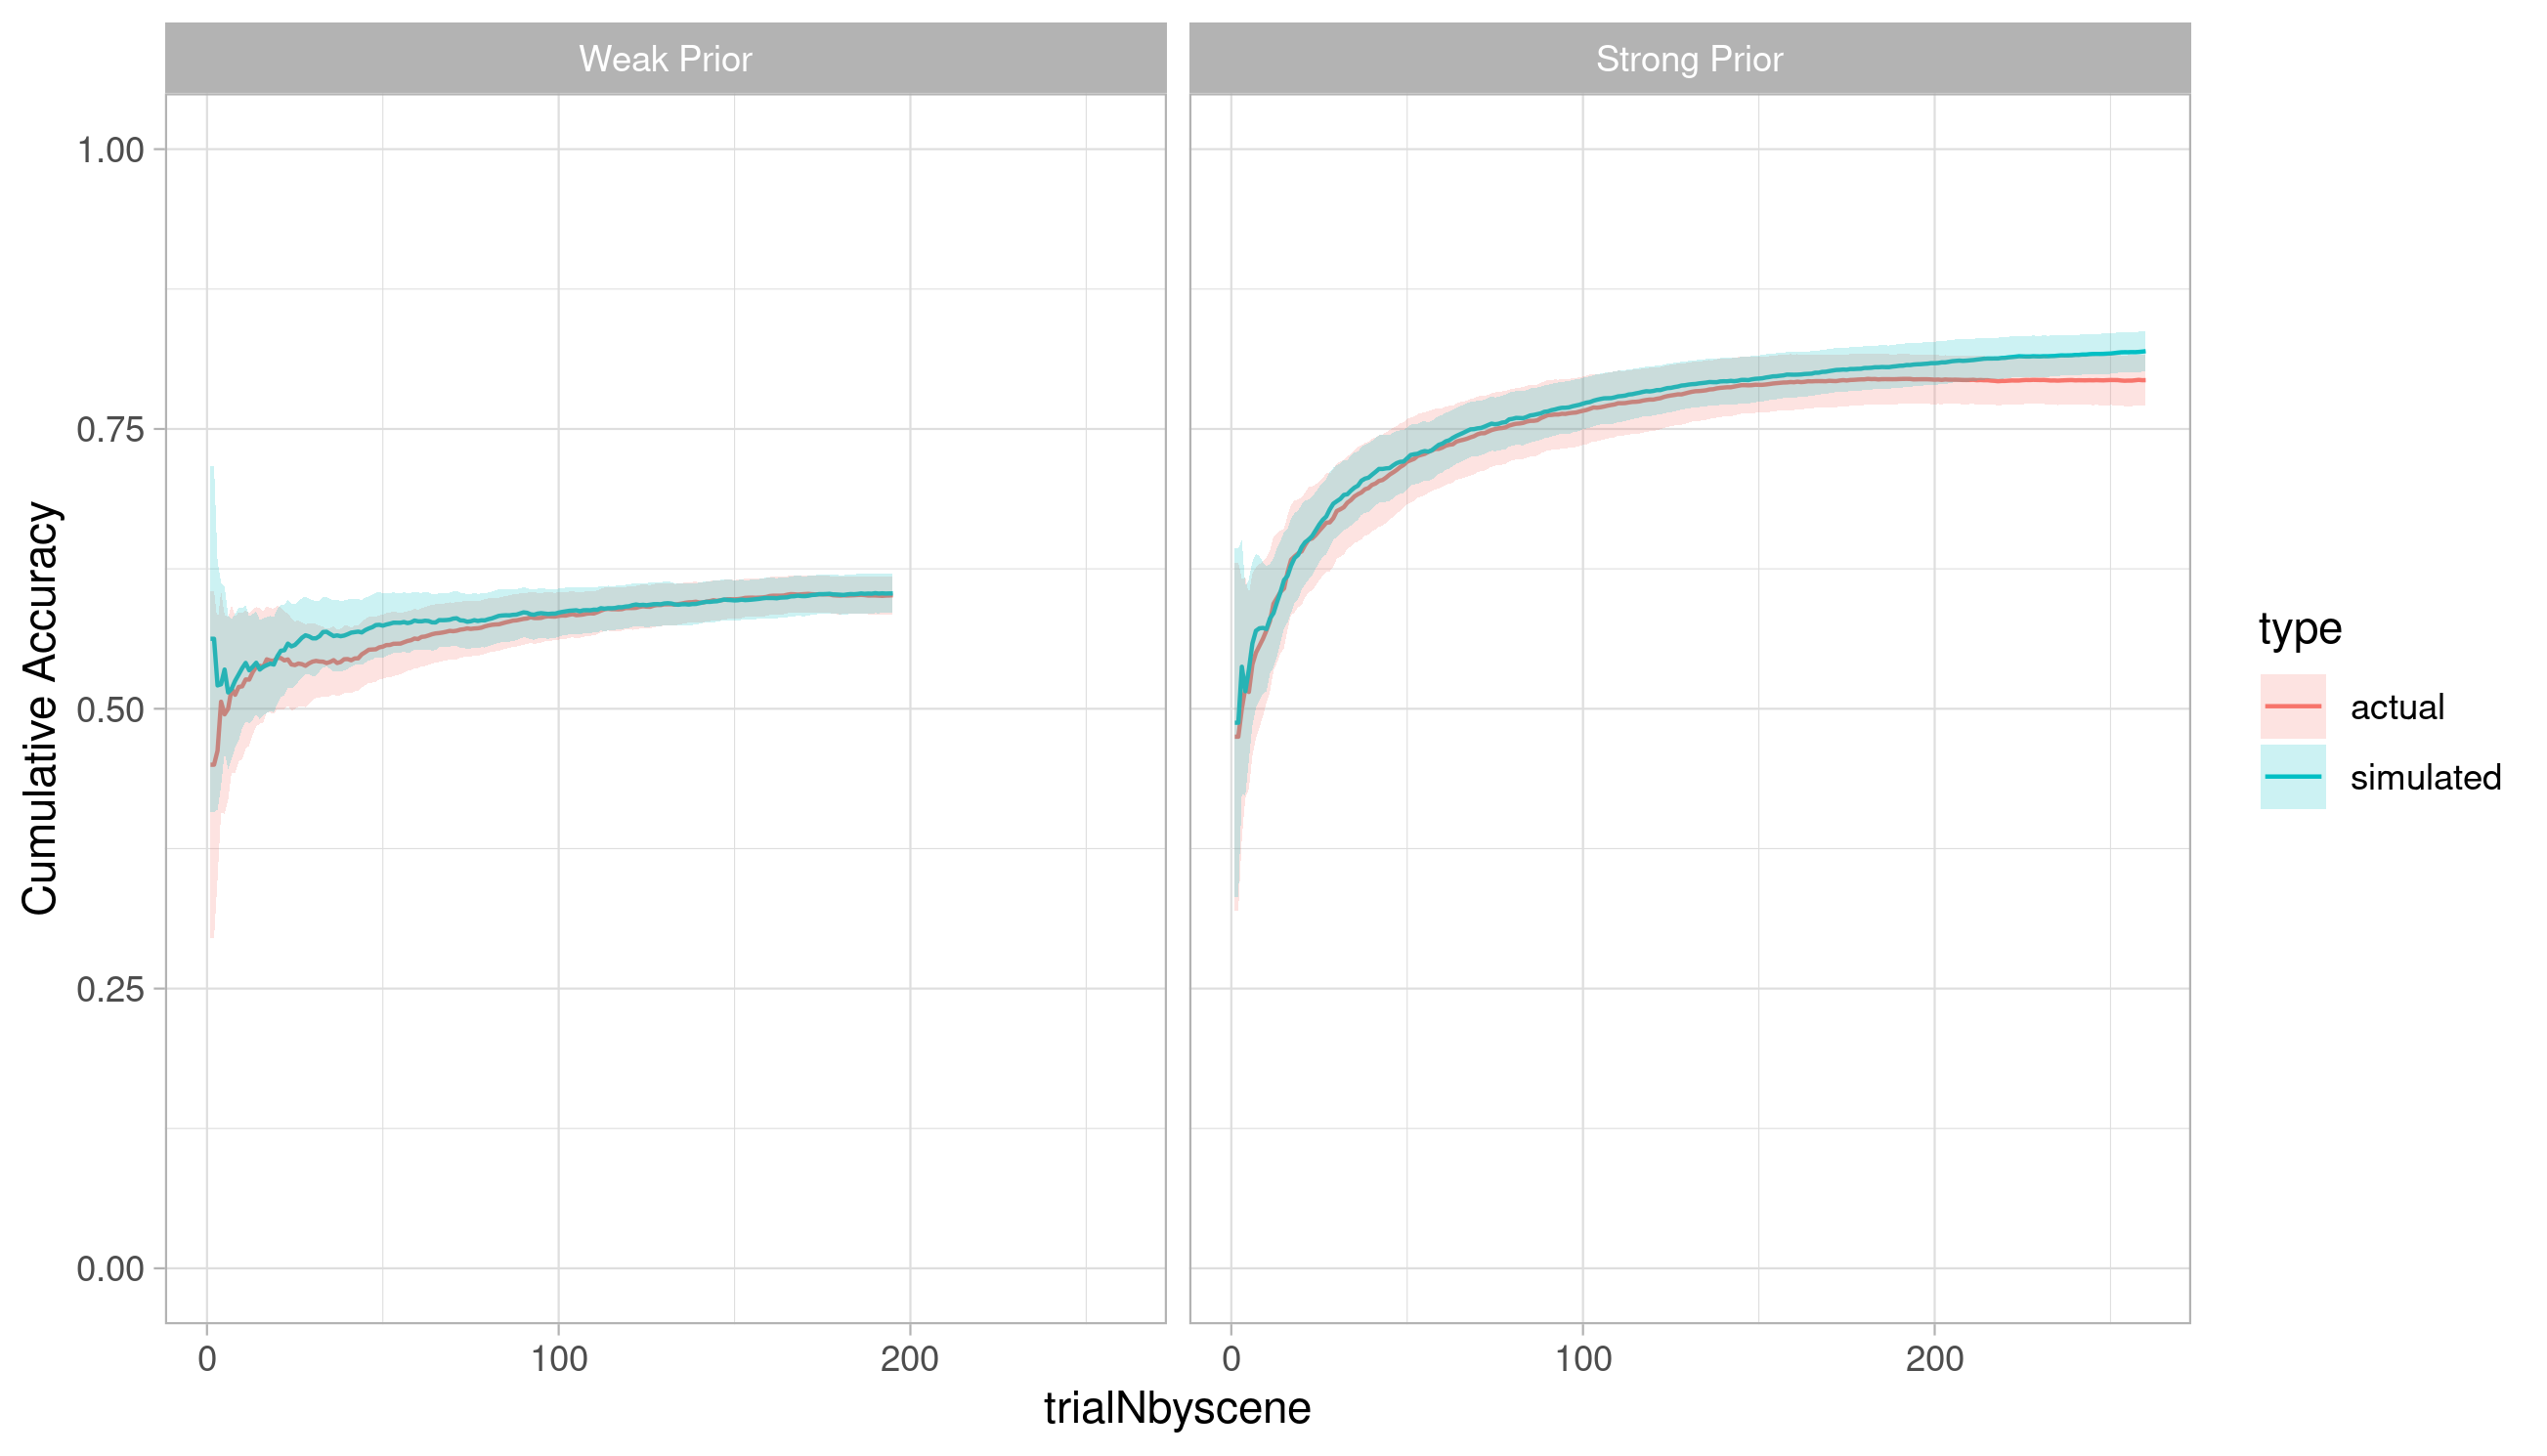
\includegraphics[width=1.5\textwidth]{figures/SimulatedVsActual.exp=exp2.mod=fLR_Instr.png}}
\caption{\textbf{Simulated vs Empirical Data - Experiment 2.} Simulated data (red line) and actual data (green line) overlapped, for experiment 2, for weak priors condition and strong prior condition. }
\label{fig:simvsemp_Exp2}
\end{figure}

In addition, to check whether the model captured participants' differences in learning rate, we compared cumulative accuracy for simulated and empirical data at different values of learning rate $\alpha$. For simulated and empirical data, quartiles for $\alpha$ were calculated (zeroth, first, second, third, and fourth quartile), and cumulative accuracy was aggregated for the data points between one quartile and the previous one. Cumulative accuracy for the four bins created is shown in Figure \ref{fig:binAll}, as a function of order of the trials (late vs early), type of data (empirical vs simulated), and experiment (first vs second experiment). For both actual and simulated data, a higher learning rate was more beneficial than a lower one for early trials, while on late trials higher learning rates are detrimental for the learning task. These effects seem not to vary substantially as a function of the experiment. 

\begin{figure}[ht!]
\centerline
{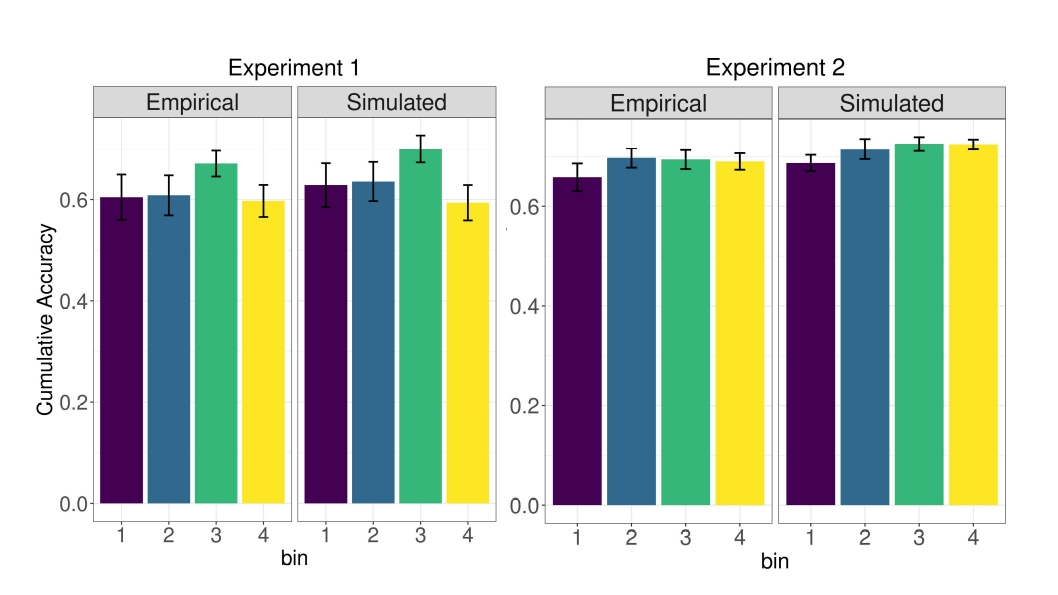
\includegraphics[width=1.5\textwidth]{figures/bin.plot.all.jpg}}
\caption{\textbf{Cumulative Accuracy for Simulated and Empirical by Learning Rate.} Figures show the cumulative accuracy at the leaning task for early vs late trials, at different learning rate levels, for a) experiment 1 and b) experiment two. Cumulative accuracy was binned  }
\label{fig:binAll}
\end{figure}

\subsection{Recognition Memory Results}
To evaluate overall memory performance for each participant, a d' score was calculated from the hits (responding "old" to old items) and false alarms (responding "old" to new items), an index which indicates participants' ability to discriminate between old and new items. In order to exclude participants who did not perform the task above chance level, we created a null distribution by generating 5000 random permutations of the trial labels. We then excluded participants whose performance was below the 95 \% percentile of the null distribution (see Fig \ref{fig:dprime}). Five participants from experiment 1 and five from experiment 2 with overall d' score below the obtained threshold were excluded from further analyses. After the exclusion, the final d' was d' = 0.93,  \textit{t}(26) = 13.7, \textit{p} < .001 for experiment 1, and d’ = 0.90,  \textit{t}(34) = 16.8, \textit{p} < .001 for experiment 2, indicating that participants were overall able to discriminate previously presented old items from new distractors. \par


\begin{figure}[ht!]
{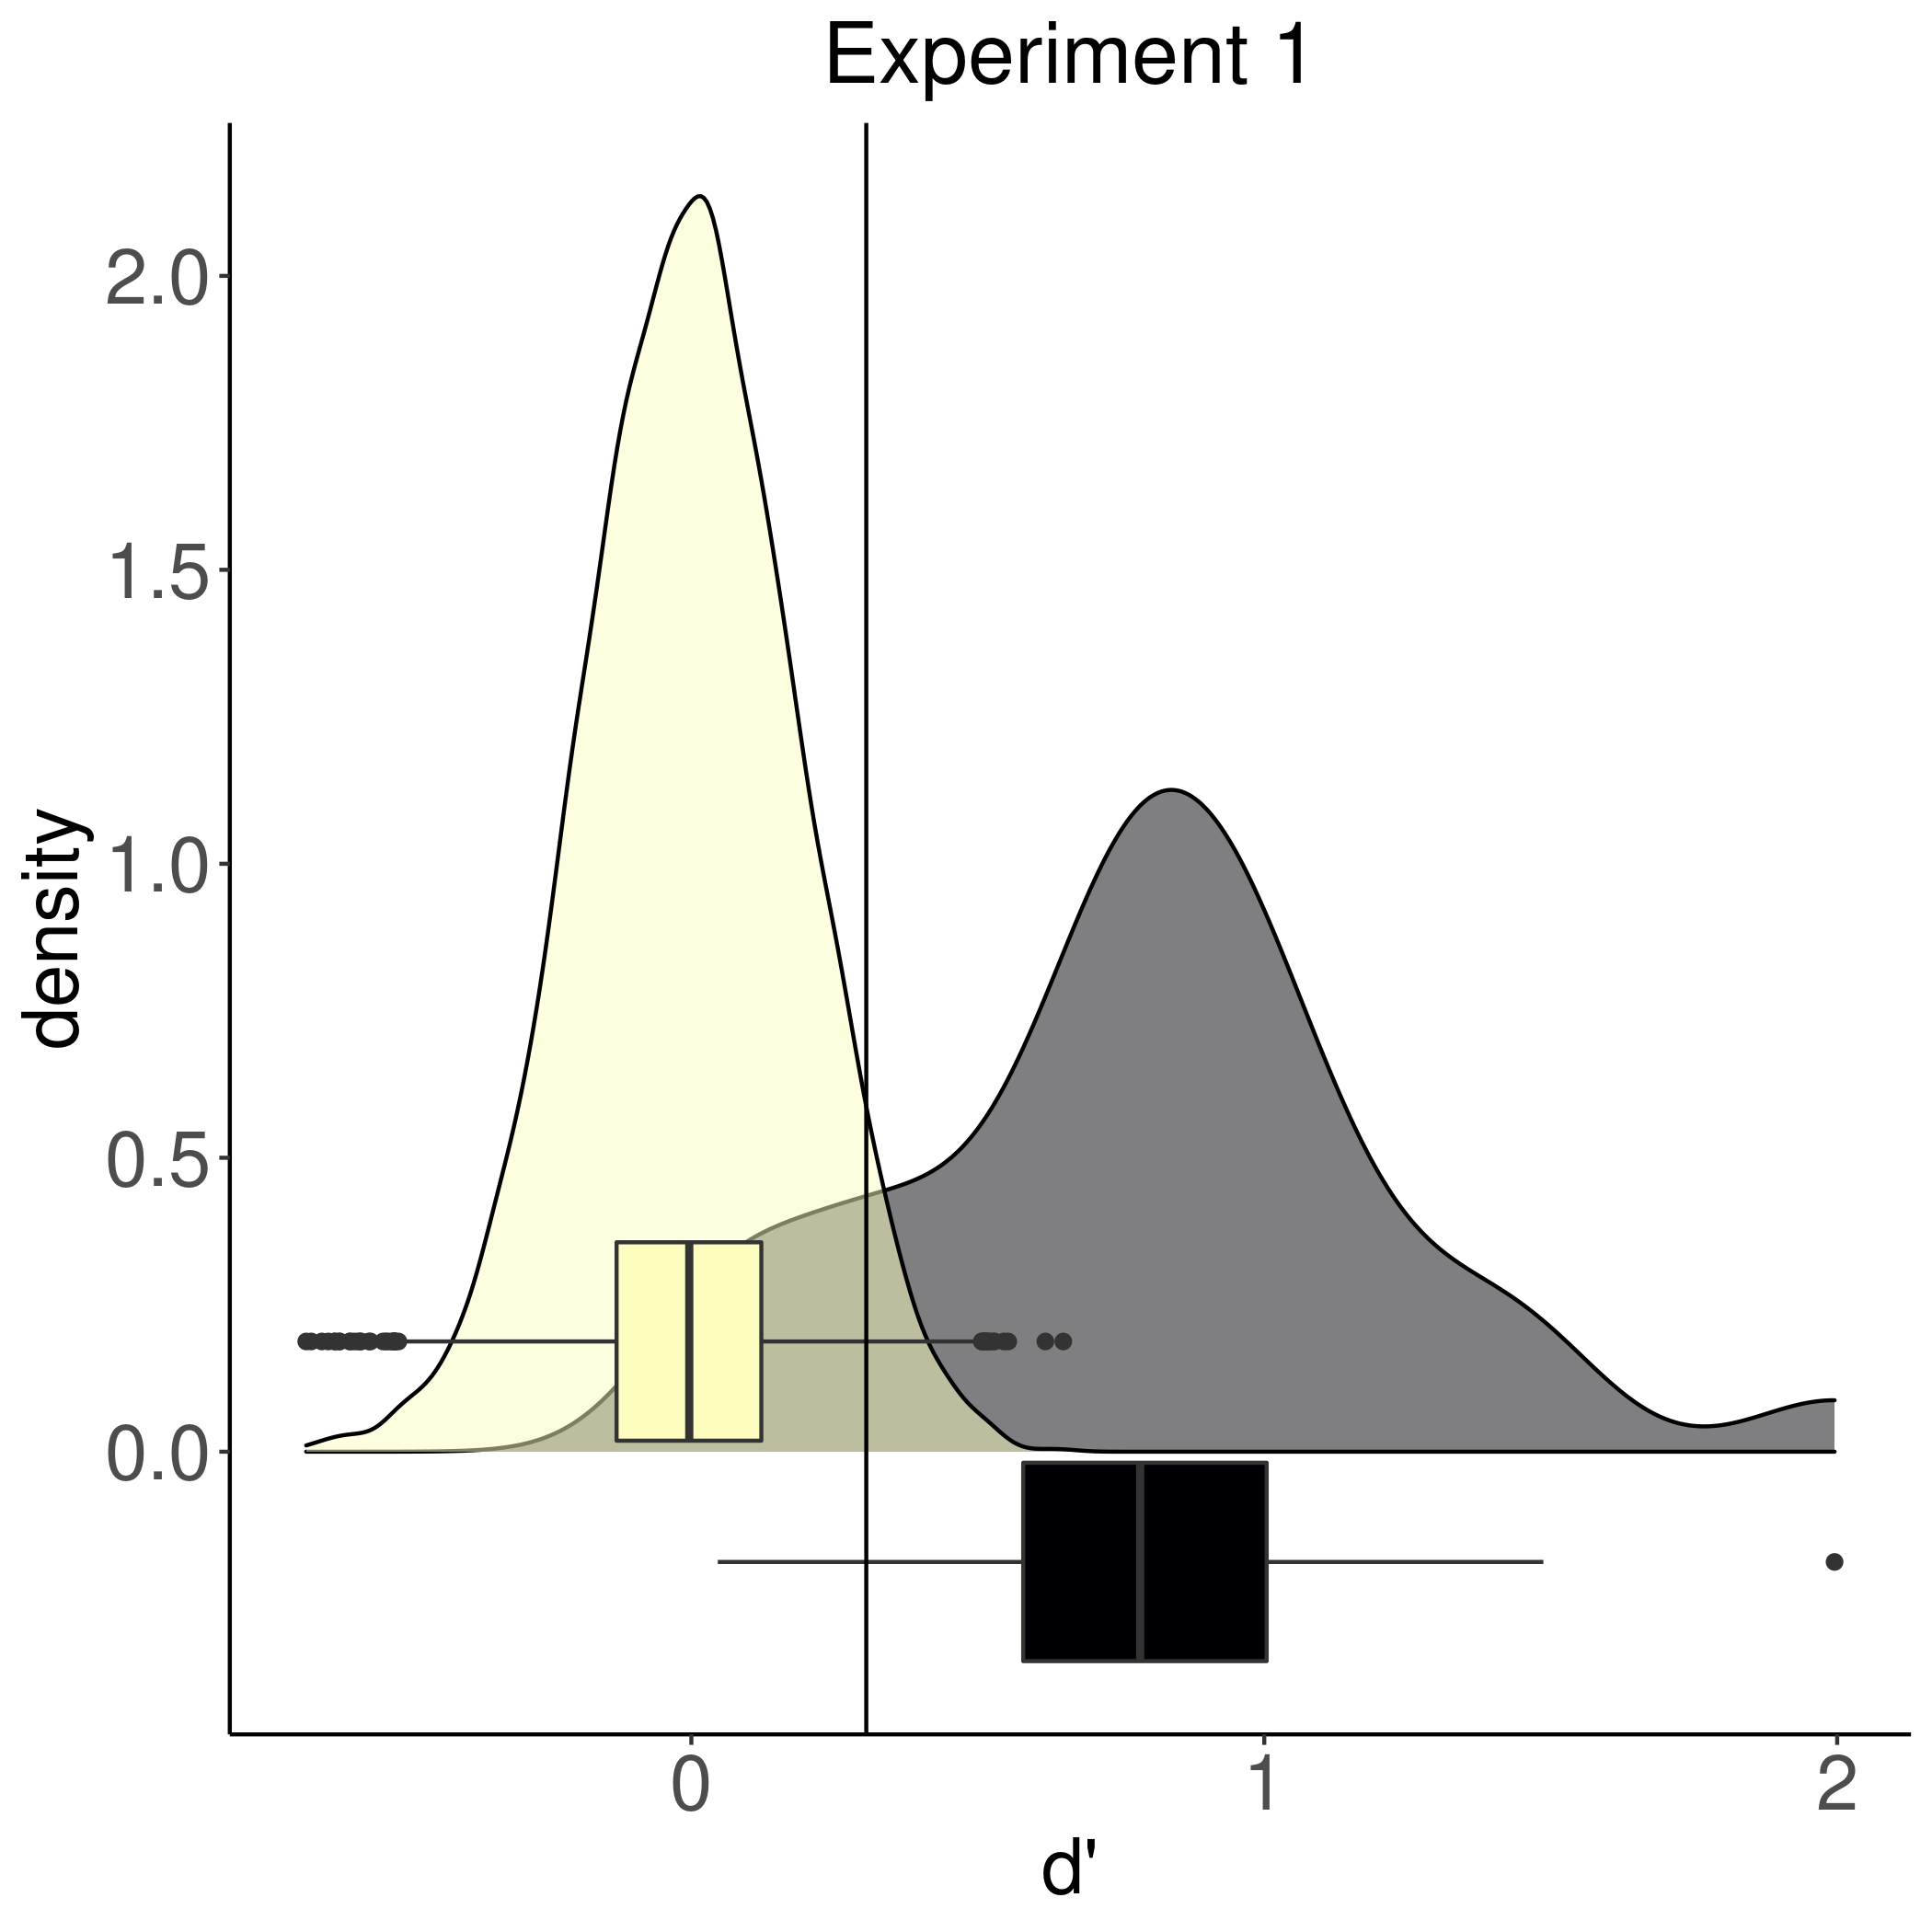
\includegraphics[width=0.5\textwidth]{figures/dprime_exp1.png}} \hfill
{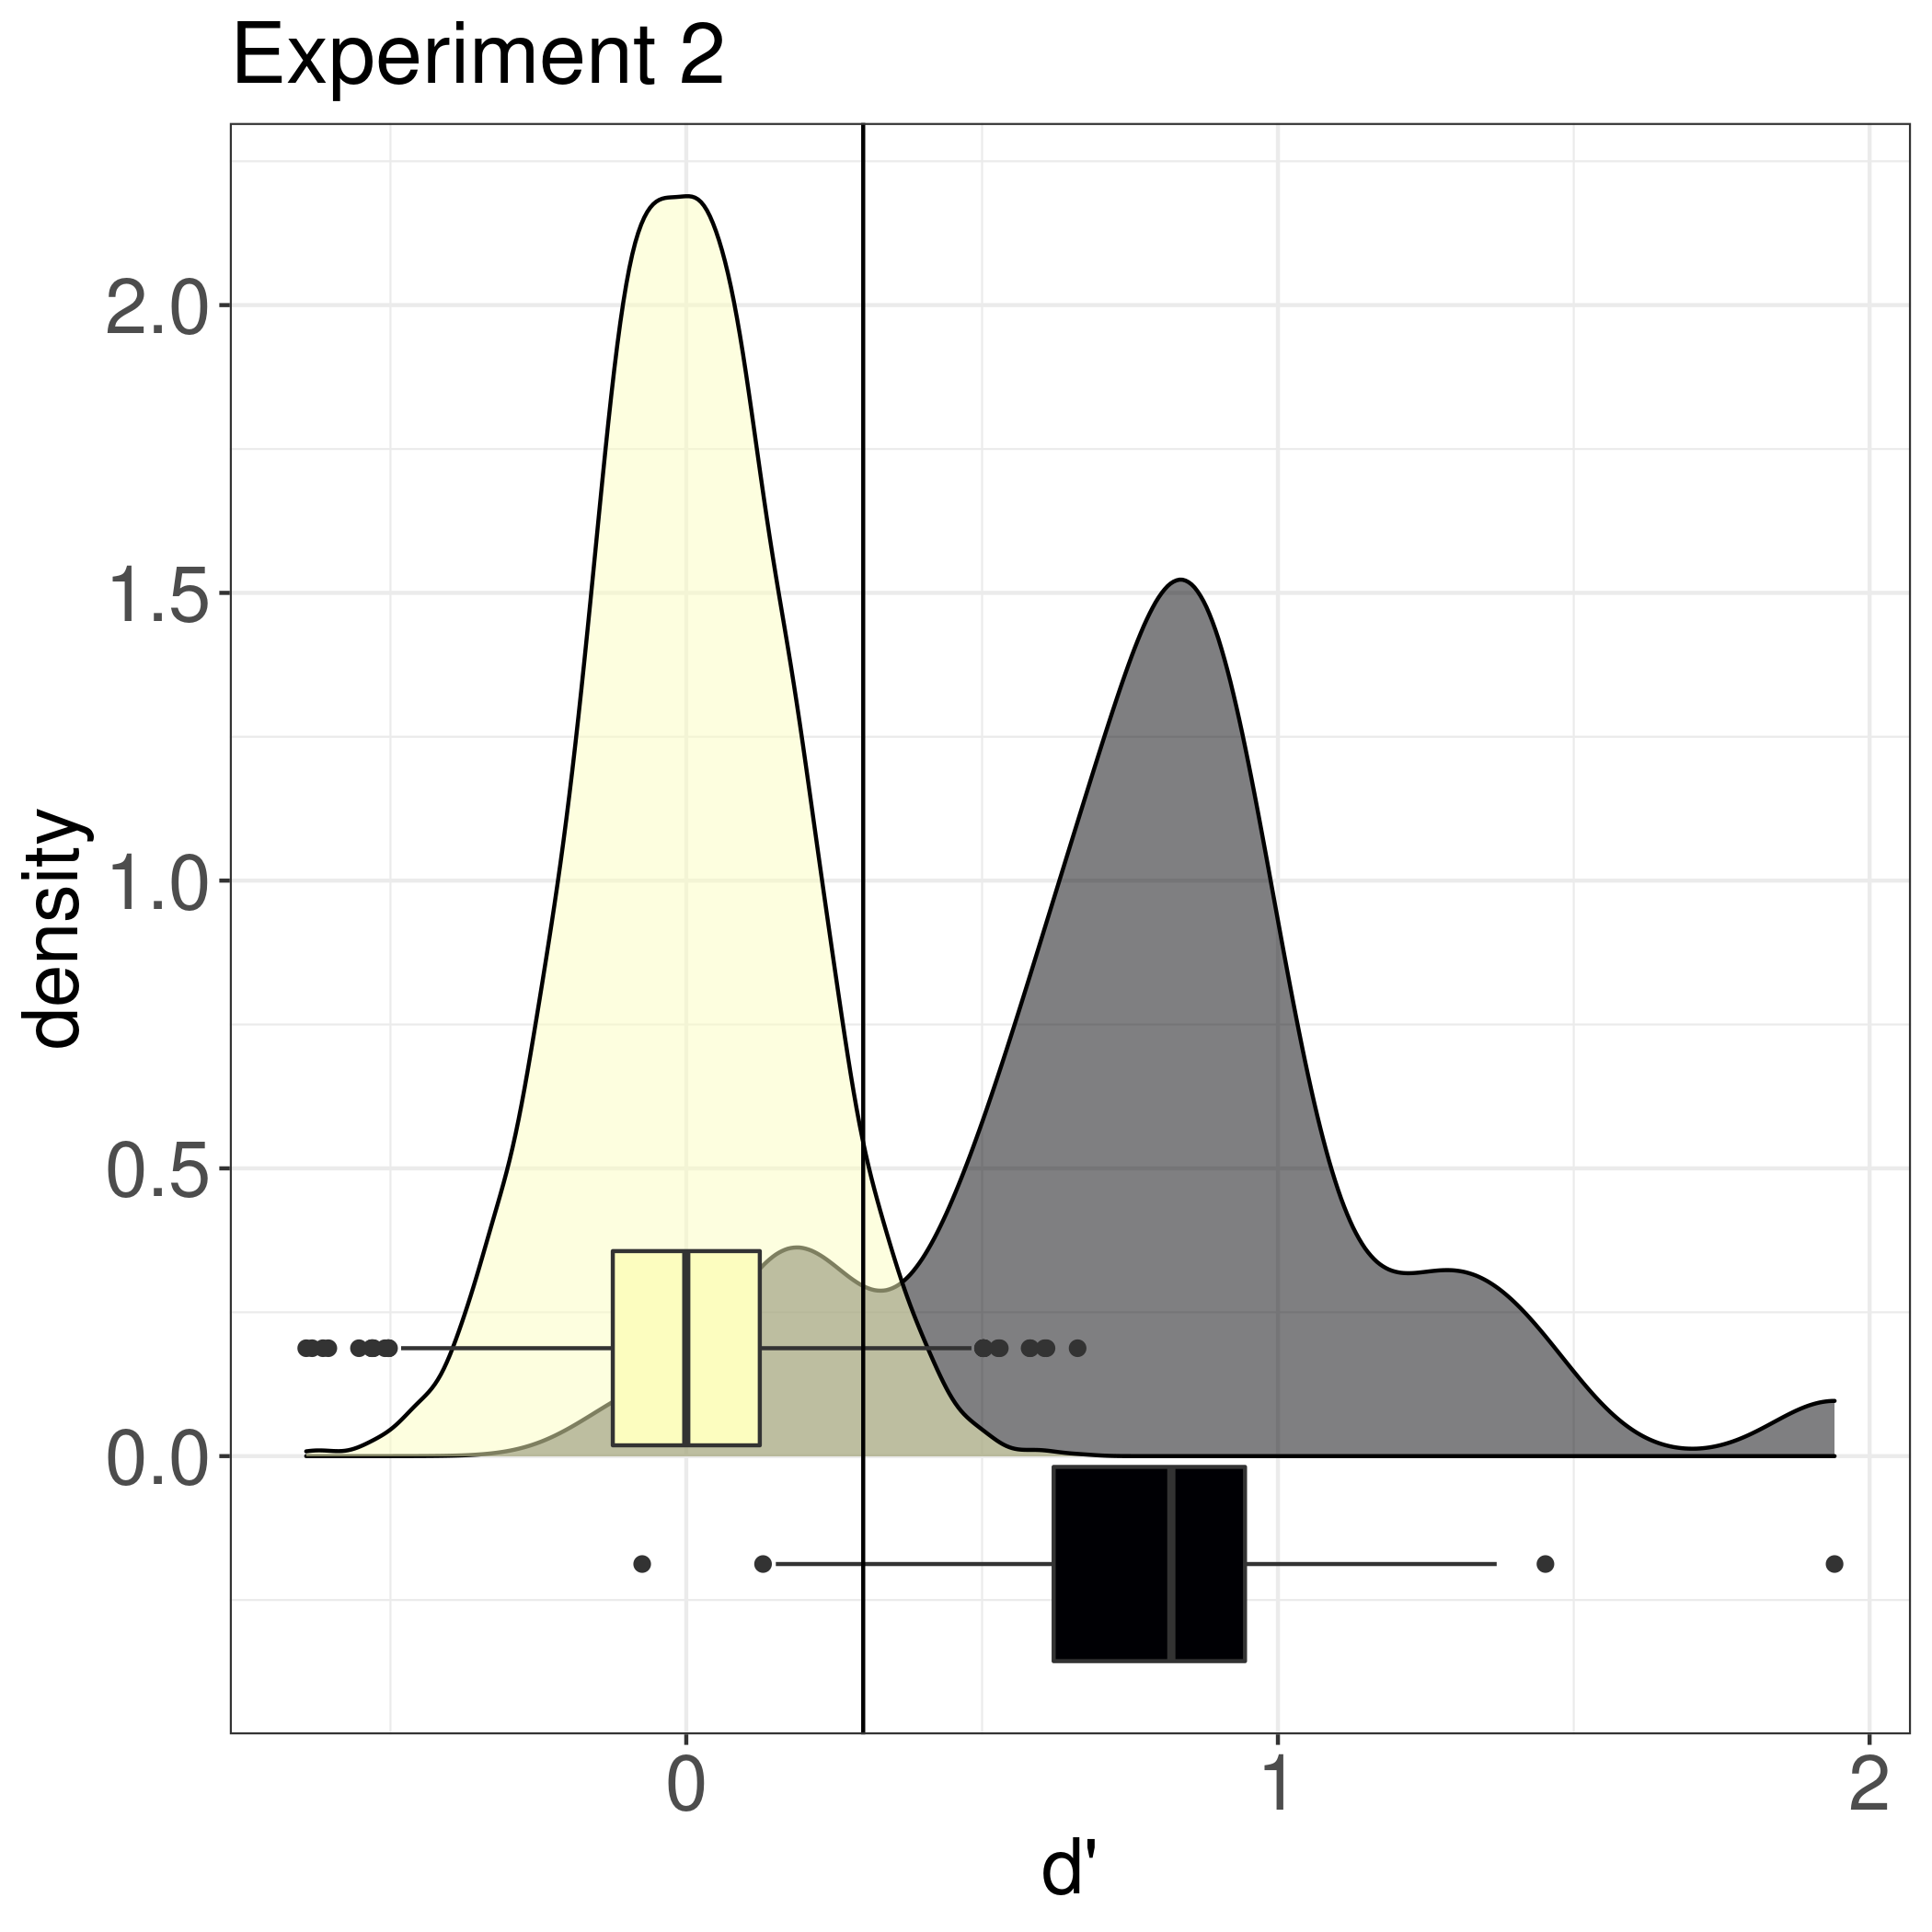
\includegraphics[width=0.5\textwidth]{figures/dprime_exp2.png}} 
\caption{\textbf{Distributions of d' by experiment.} Participants' d' distributions (on the right side of both graphs) overlayed with the null distribution created by generating 5000 random permutations (on the left side), for experiment 1 and 2. The vertical black line represents the 95 \% percentile of the null distribution. Participants' whose d' fell below that threshold were excluded from further analyses.}
\label{fig:dprime}
\end{figure}

We then tested whether prediction outcome (correct vs incorrect) influenced recognition accuracy. A graph of recognition accuracy as a function prediction outcome is shown in \ref{fig:prediction_cond}. In both experiment, there was no significant effect of prediction outcome on recognition accuracy (Experiment 1: $\chi^2_{(1)}$ = 1.27, \textit{p} = .259; Experiment 2: $\chi^2_{(1)}$ = 2.09, \textit{p} = .148.


\begin{figure}[ht!]
{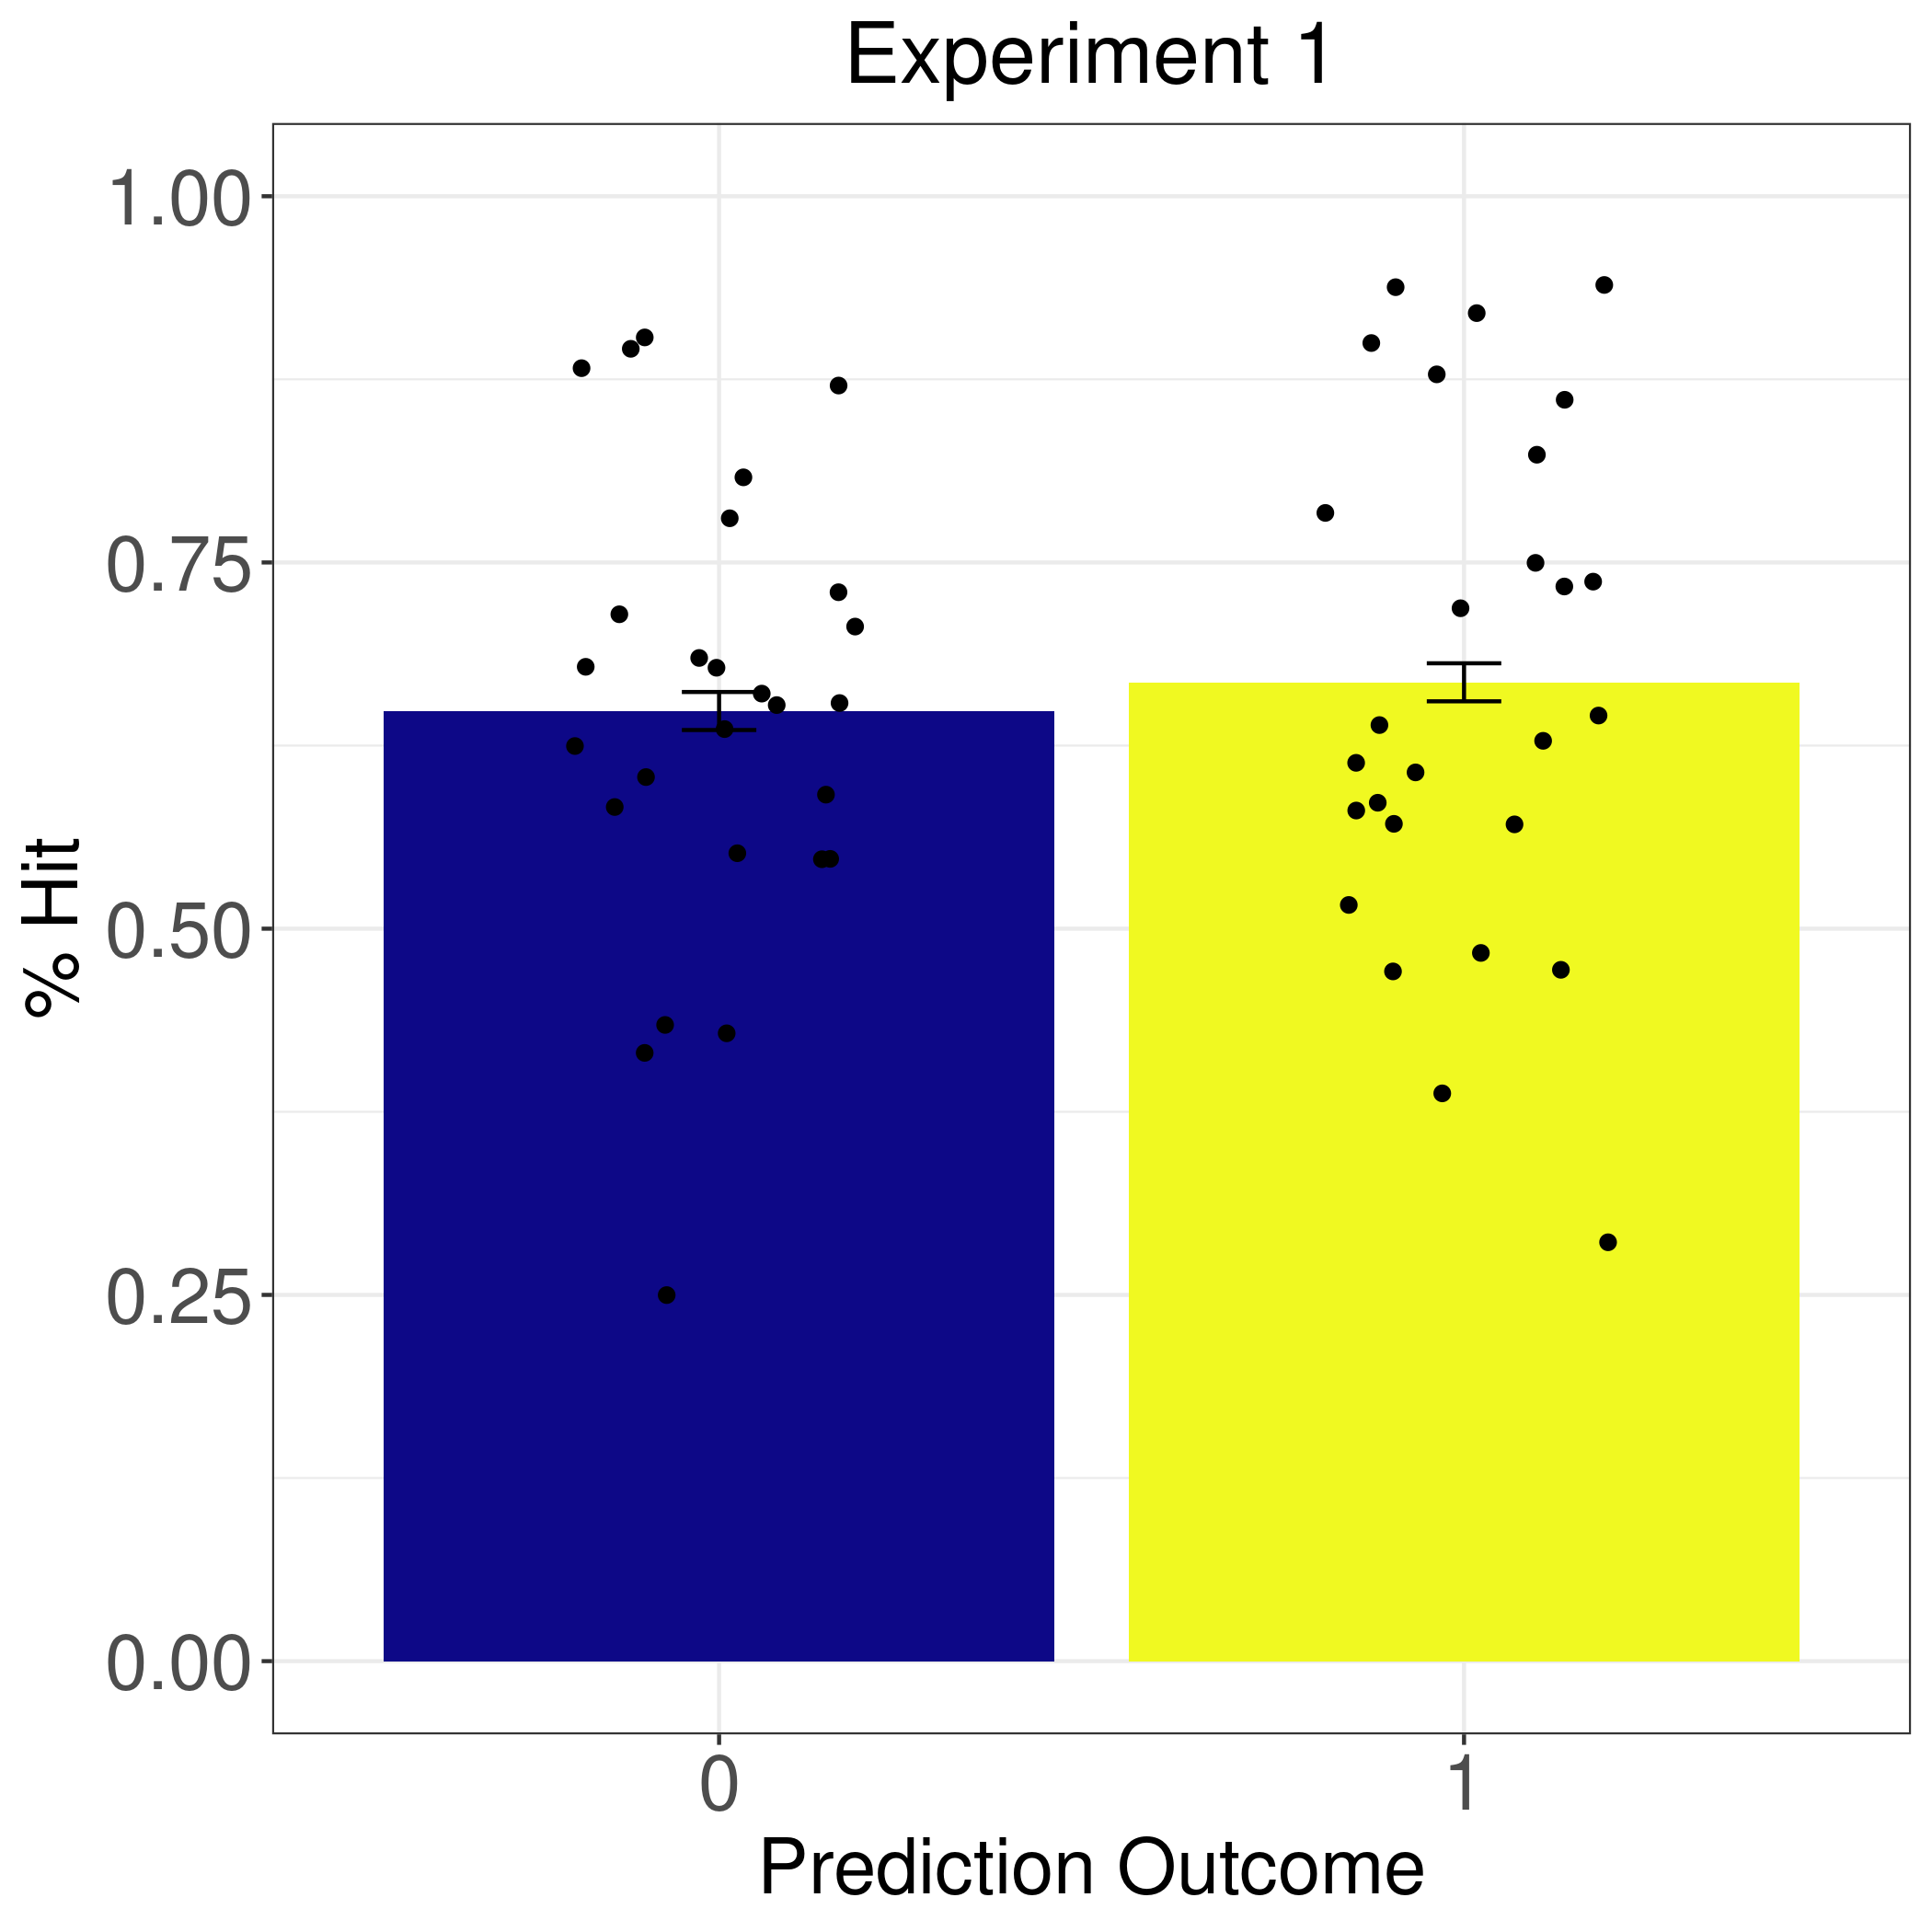
\includegraphics[width=0.5\textwidth]{figures/prediction_acc_exp1.png}} \hfill
{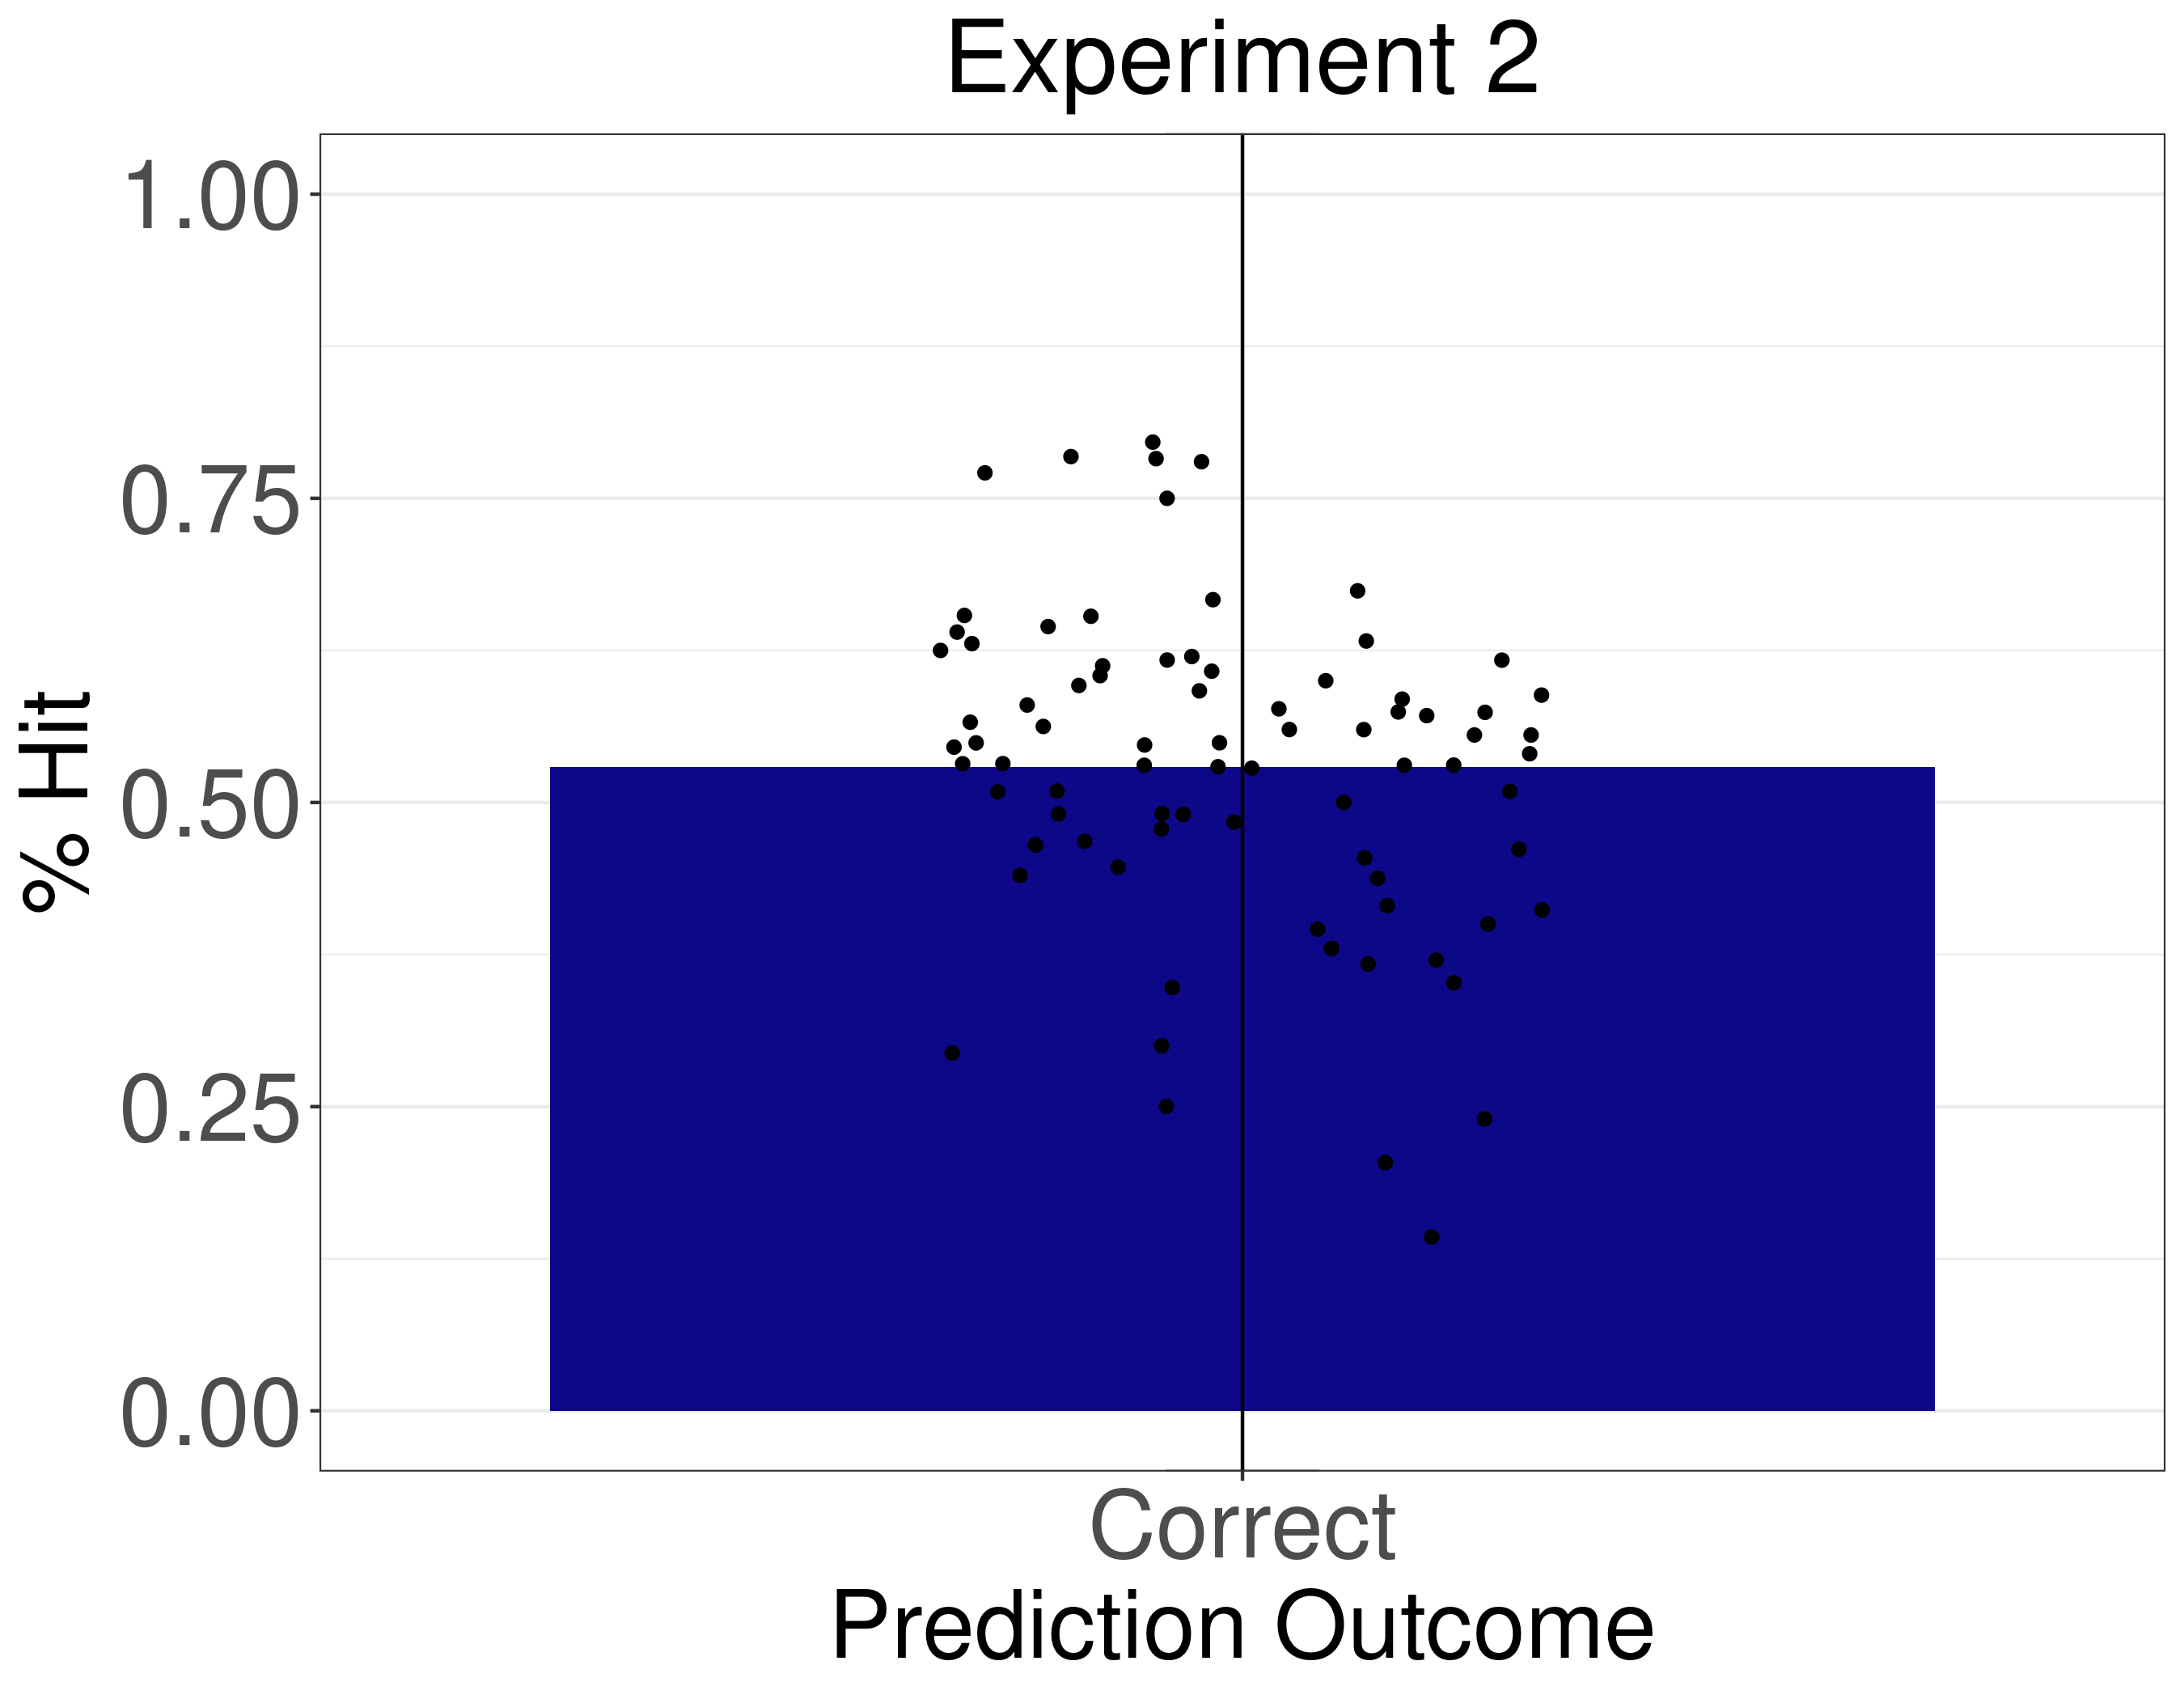
\includegraphics[width=0.5\textwidth]{figures/prediction_acc_exp2.png}} 
\caption{\textbf{Recognition accuracy as a function of prediction outcome.}
Participants' recognition accuracy for correct and incorrect predictions in the learning task, for Experiment 1 and 2. }
\label{fig:prediction_cond}
\end{figure}

\subsection{Memory as a function of model-derived PE}
The fLRI model was fit to participant data with the estimated best fit parameter in order to derive trial-level PE during the encoding phase. PE was calculated as the difference between whether or not an object category was presented (1 or 0, respectively) and its current estimated value (the strength of the expectation that an object category would be presented at a given scene). Higher PE levels were generated when a category presented was not expected, as reflected by its corresponding expected value being close to zero. By contrast, lower PE was generated by trials in which the category presented was characterized by a high expected value. As the two experiments were conceptually identical, the remaining analyses are run on data collapsed across them. Distribution of PE by contingency collapsed across experiments is shown in Figure \ref{fig:PE_distr}. 

\begin{figure}[ht!]
%\centerline
{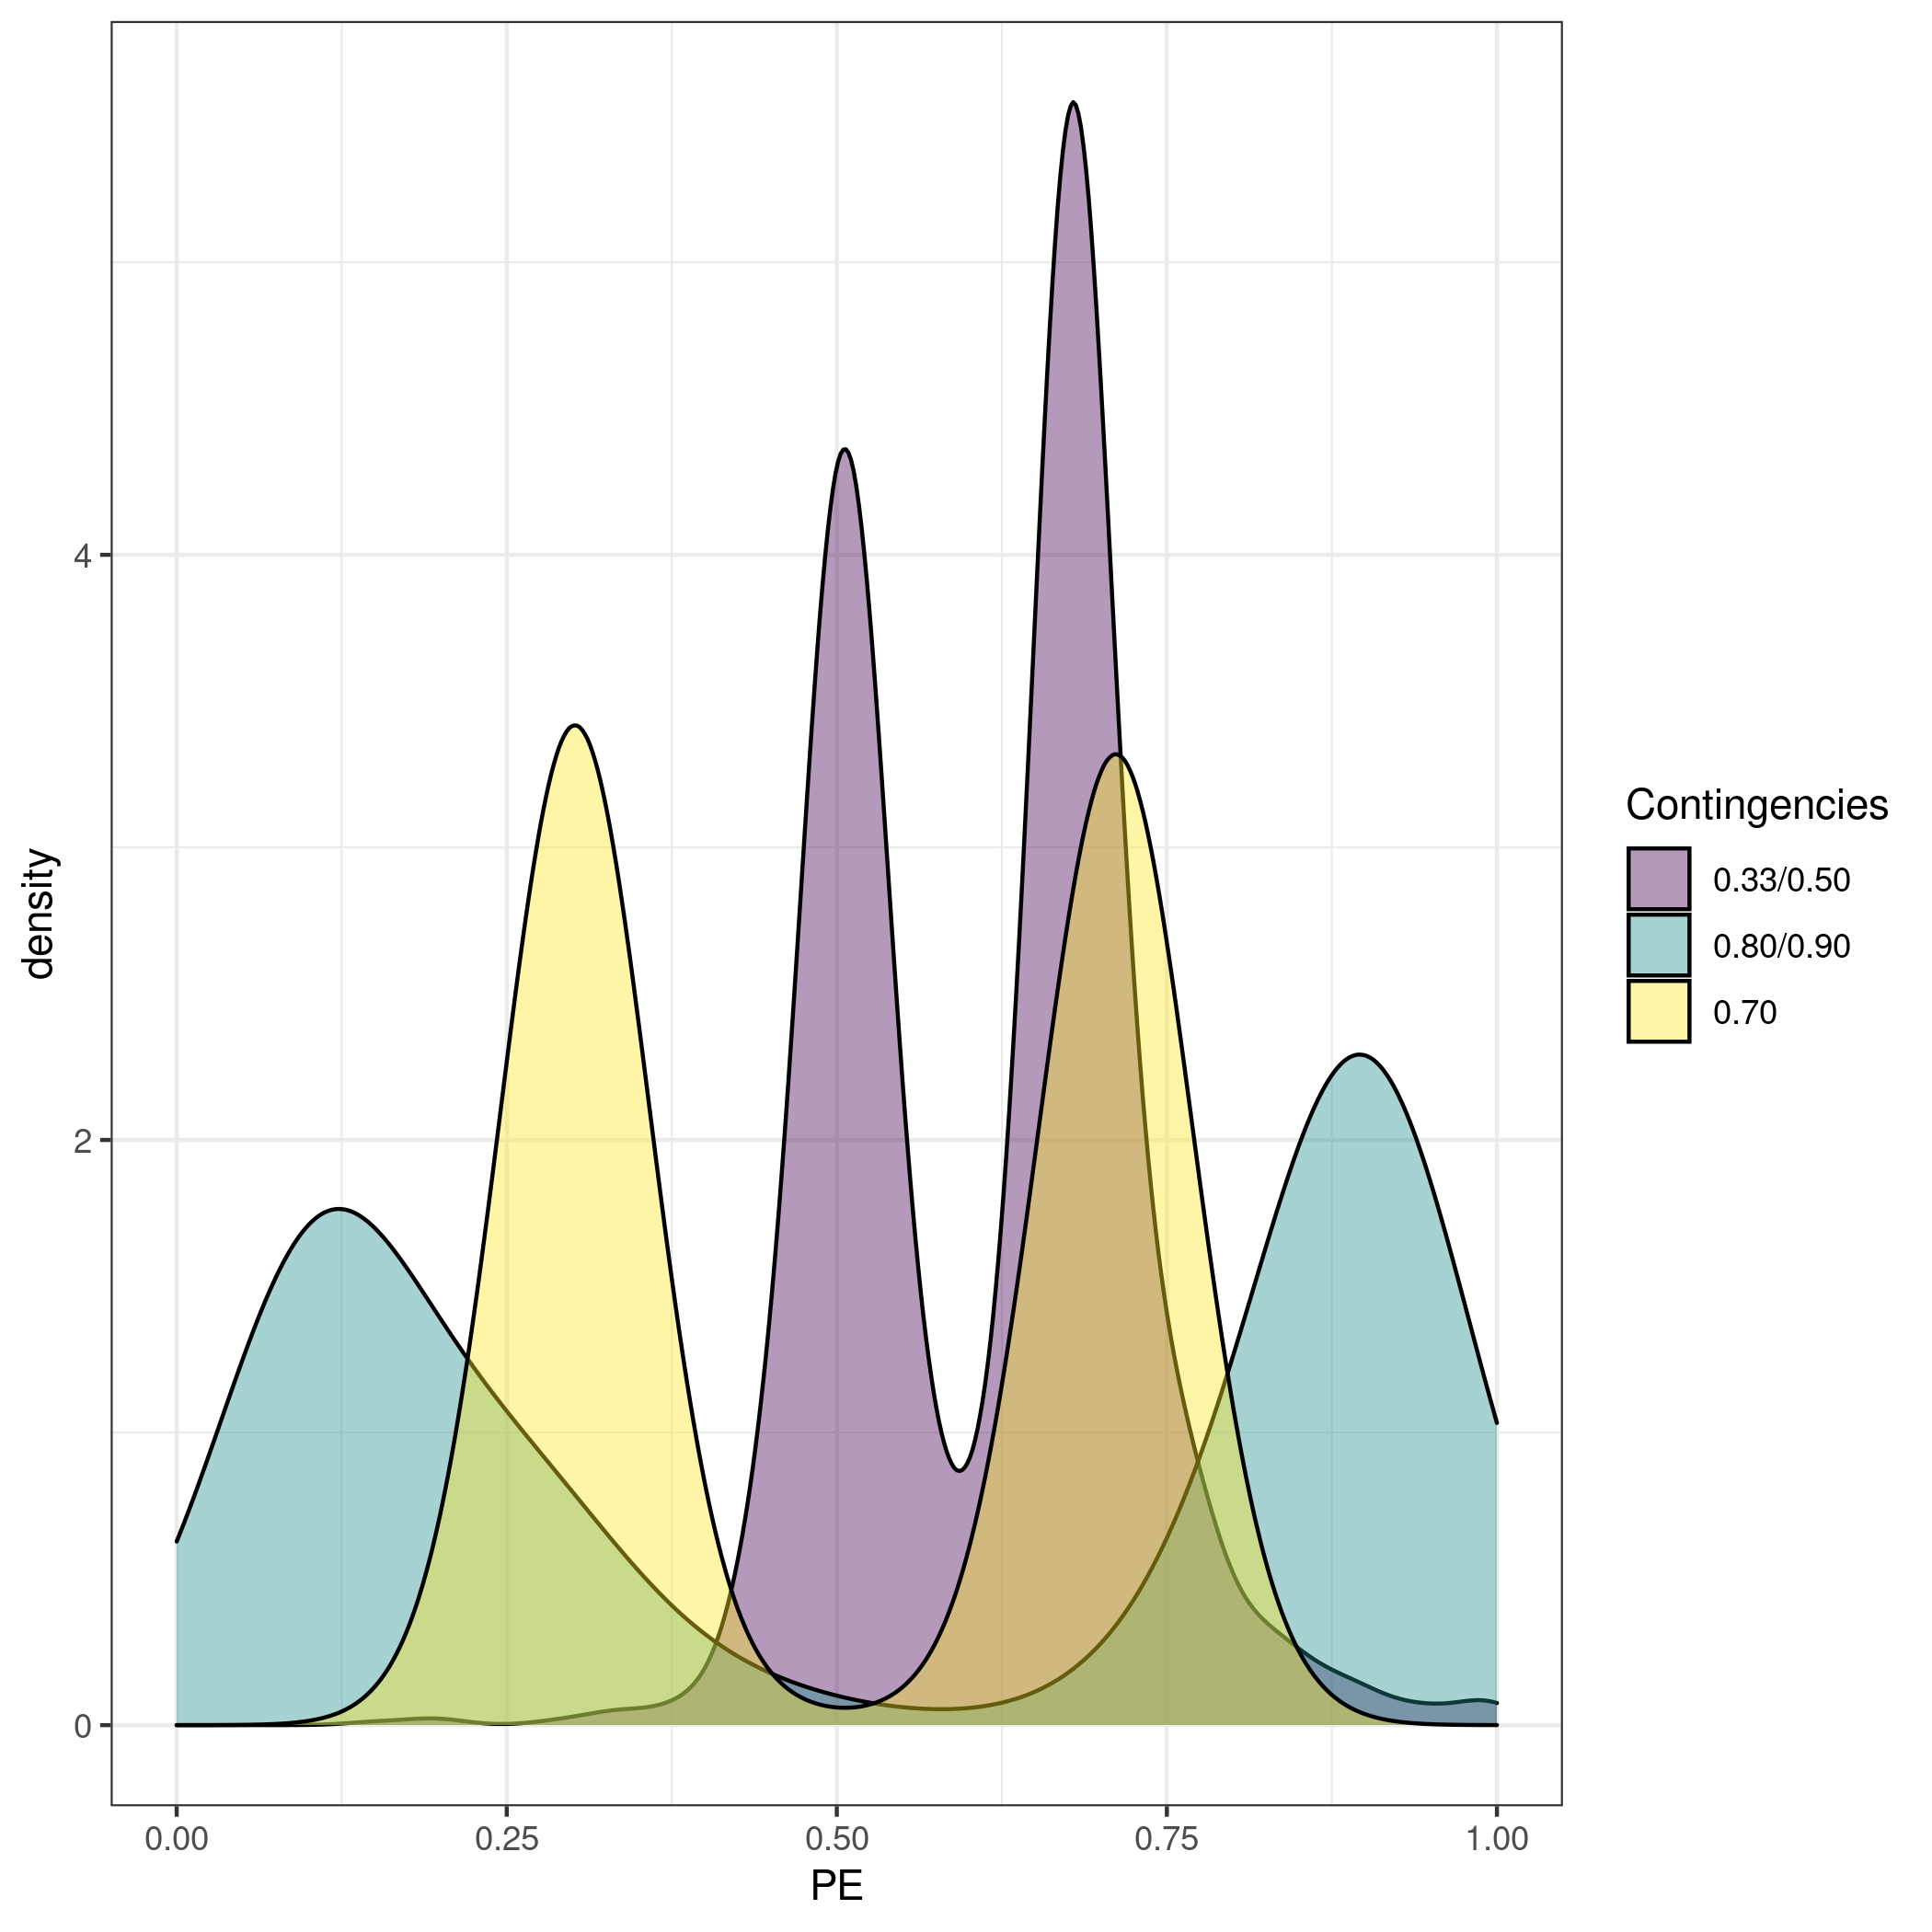
\includegraphics[width=0.5\textwidth]{figures/PE_instr_distr.exp1.exp2.png}} \hfill
{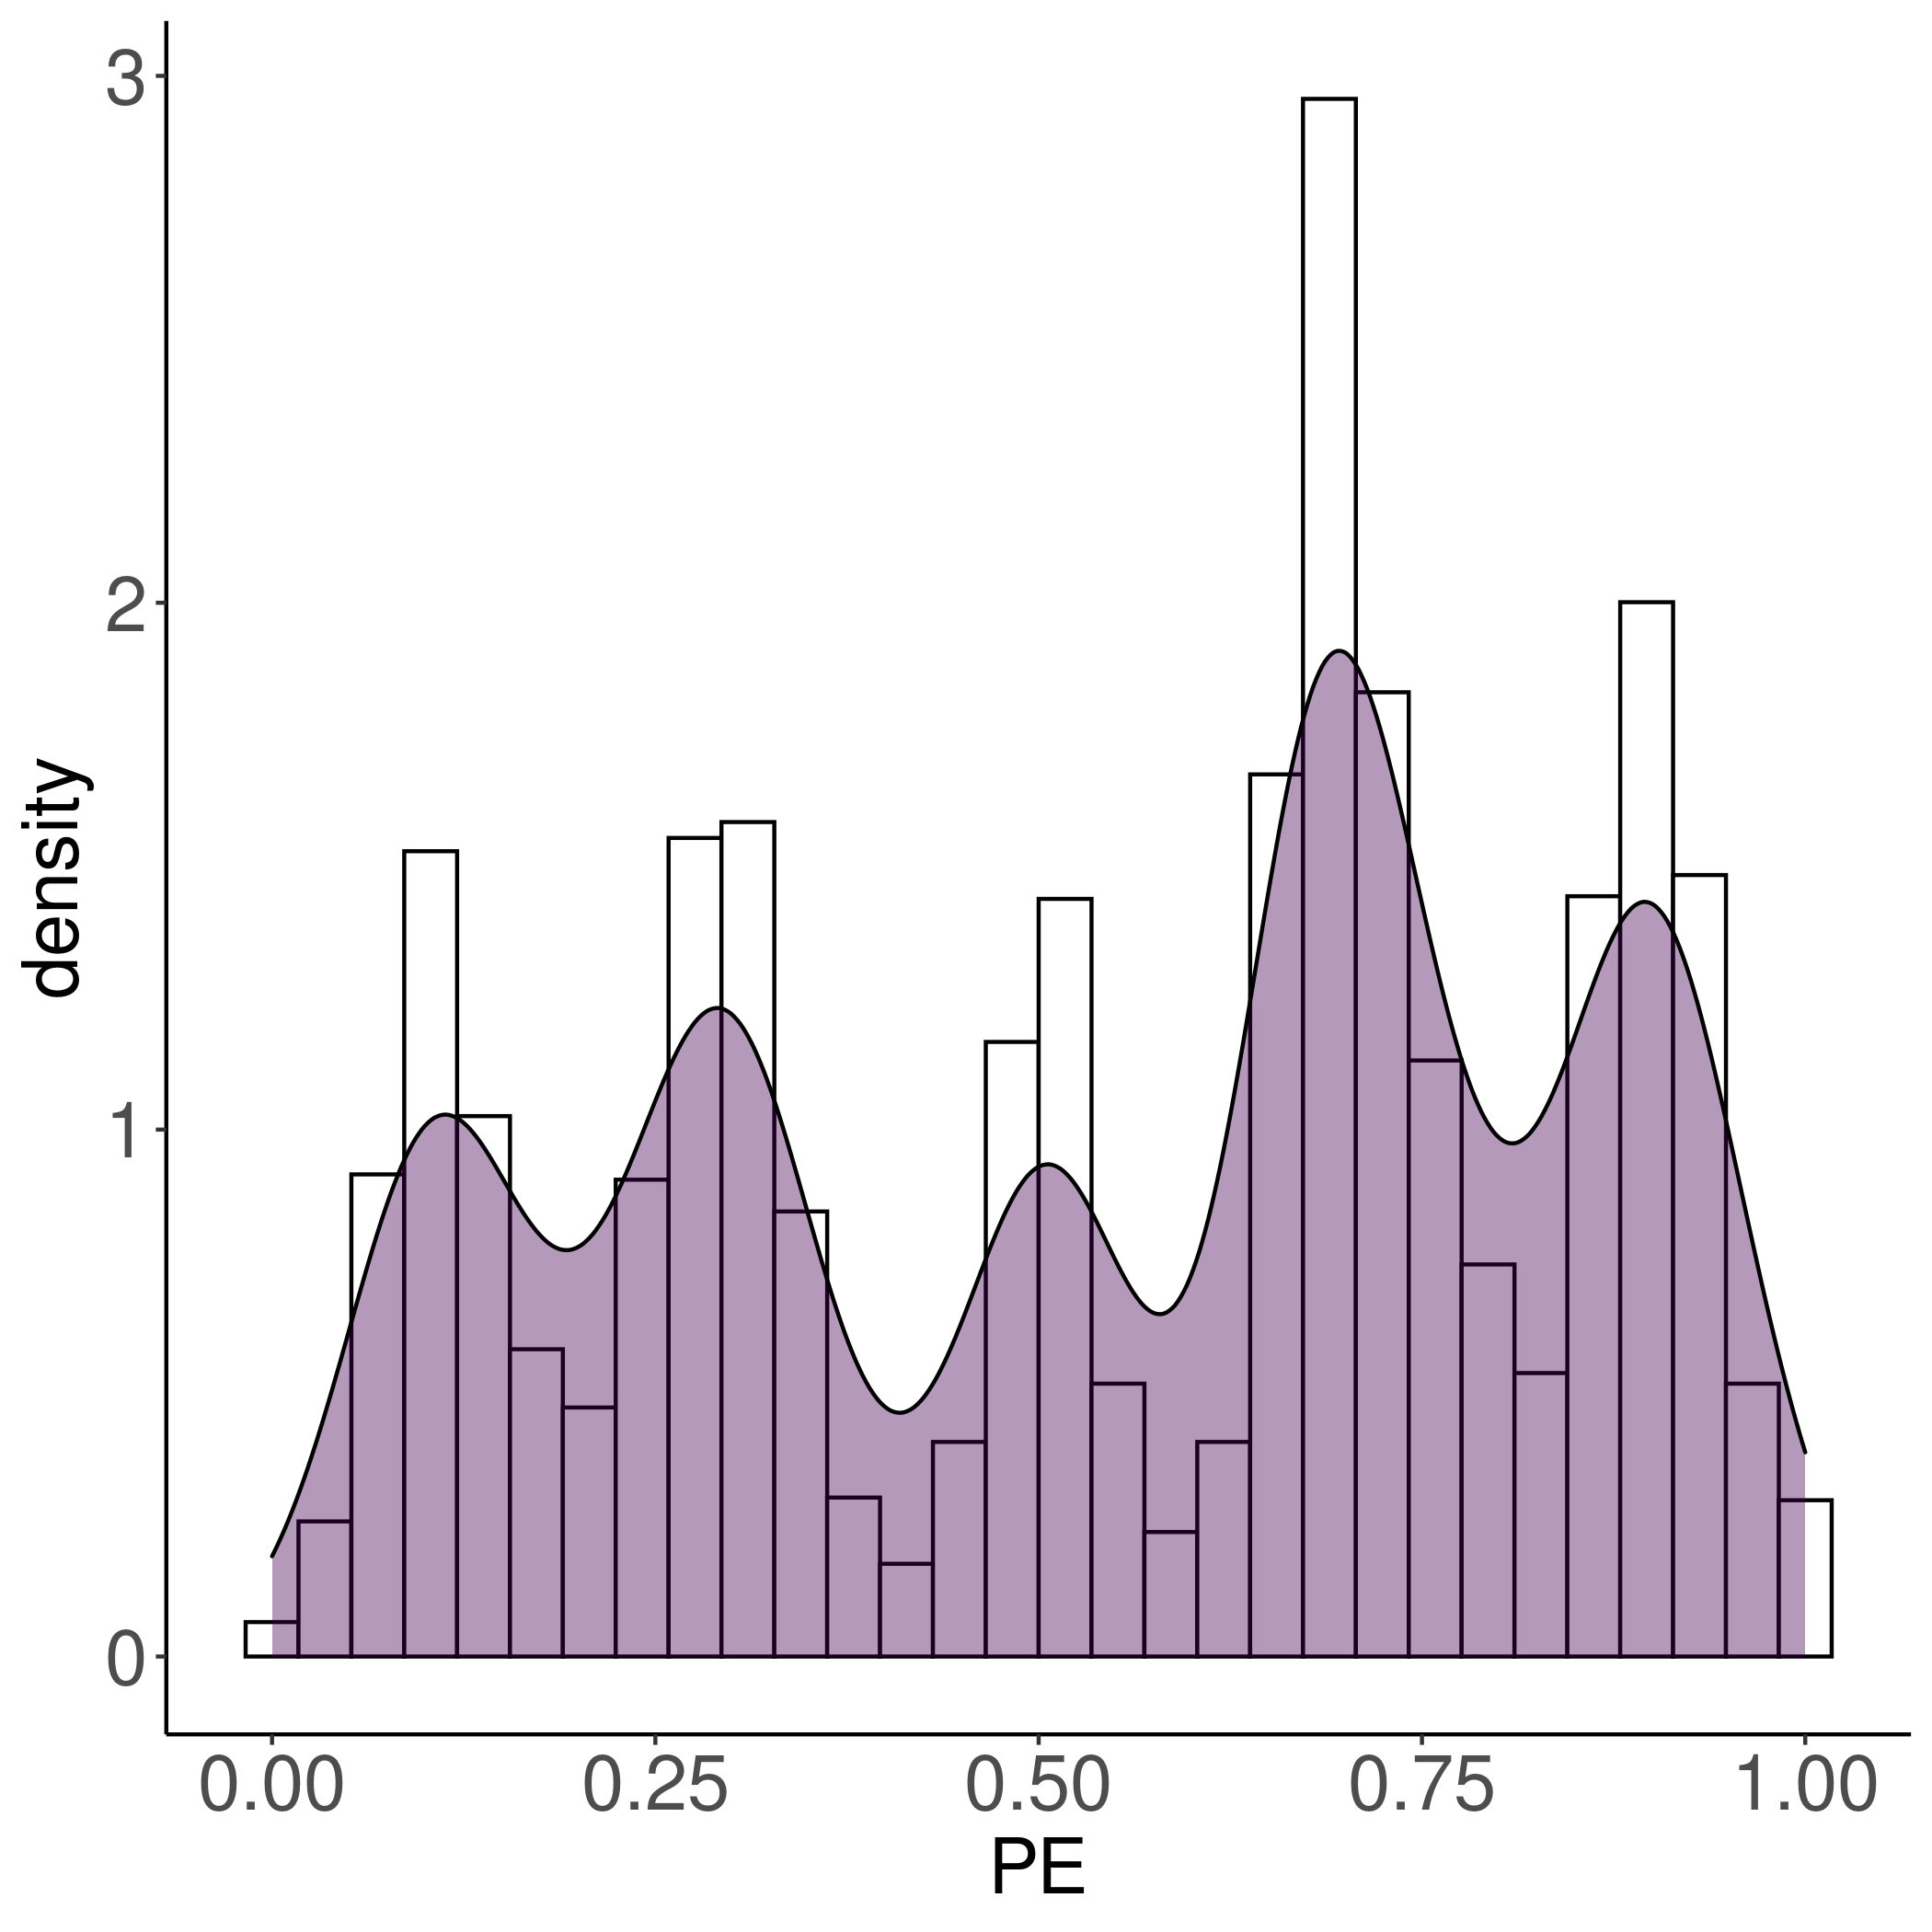
\includegraphics[width=0.5\textwidth]{figures/PE_instr_distrNOscene.exp1.exp2.png}}
\caption{\textbf{Distribution of PE by Contingency.} Figures show the density plots of model-derived PE for the different scene conditions.  }
\label{fig:PE_distr}
\end{figure}

%The plots show that PE was distributed differently as a function of the scene condition. The bimodal distribution in the weak and the strong prior conditions reflects whether or not the expectations were met at item presentation: Items that matched expectations generated distributions of PE centered at lower values, while items that mismatched expectation generated PE distributions centered at higher values. For flat prior conditions, the distribution of PE was centered at one minus the probability that an object-category was presented without considering any given condition (1-0.33 for Experiment 1, 1-0.50 for Experiment 2).
%The accuracy of the prediction was also considered, to check whether the effect of PE changed depending on whether participants' predictions were correct or not. Distribution of PE as a function of prediction outcome is shown in figure \ref{fig:PE_SC:acc}. Higher values of PE for incorrect predictions are more represented in the strong prior scene conditions, while higher values of PE for correct predictions are more represented in the weak and flat scene conditions.  
\par
We then tested whether model-derived PE was related to recognition memory. Plots of the observed values (see Figure \ref{fig:PE_mem}) revealed a relationship between PE and memory modulated by prediction outcome. In order to statistically test for the significance of this relationship, we used a generalized linear-mixed model were participants were treated as random effects (see Methods). In the model, PE and prediction outcome, as well as their interactions, were added as fixed effects. In addition, random slopes for PE and prediction outcome, and their interaction, were also added to the model. Analysis revealed a significant interaction between PE and prediction outcome ( $\chi^2_{(1)}$ = 10.46, \textit{p} = .001, Experiment 1;  $\chi^2_{(1)}$ = 13.74, \textit{p} < .001, Experiment 2).

 Distribution of PE by scene condition, experiment, and prediction accuracy is shown in Figure \ref{fig:PE_SC:acc}. Plots rendering the relationship between PE and memory for the merged data are shown in Figure \ref{fig:PE_Mem_1_2}.

\begin{figure}
{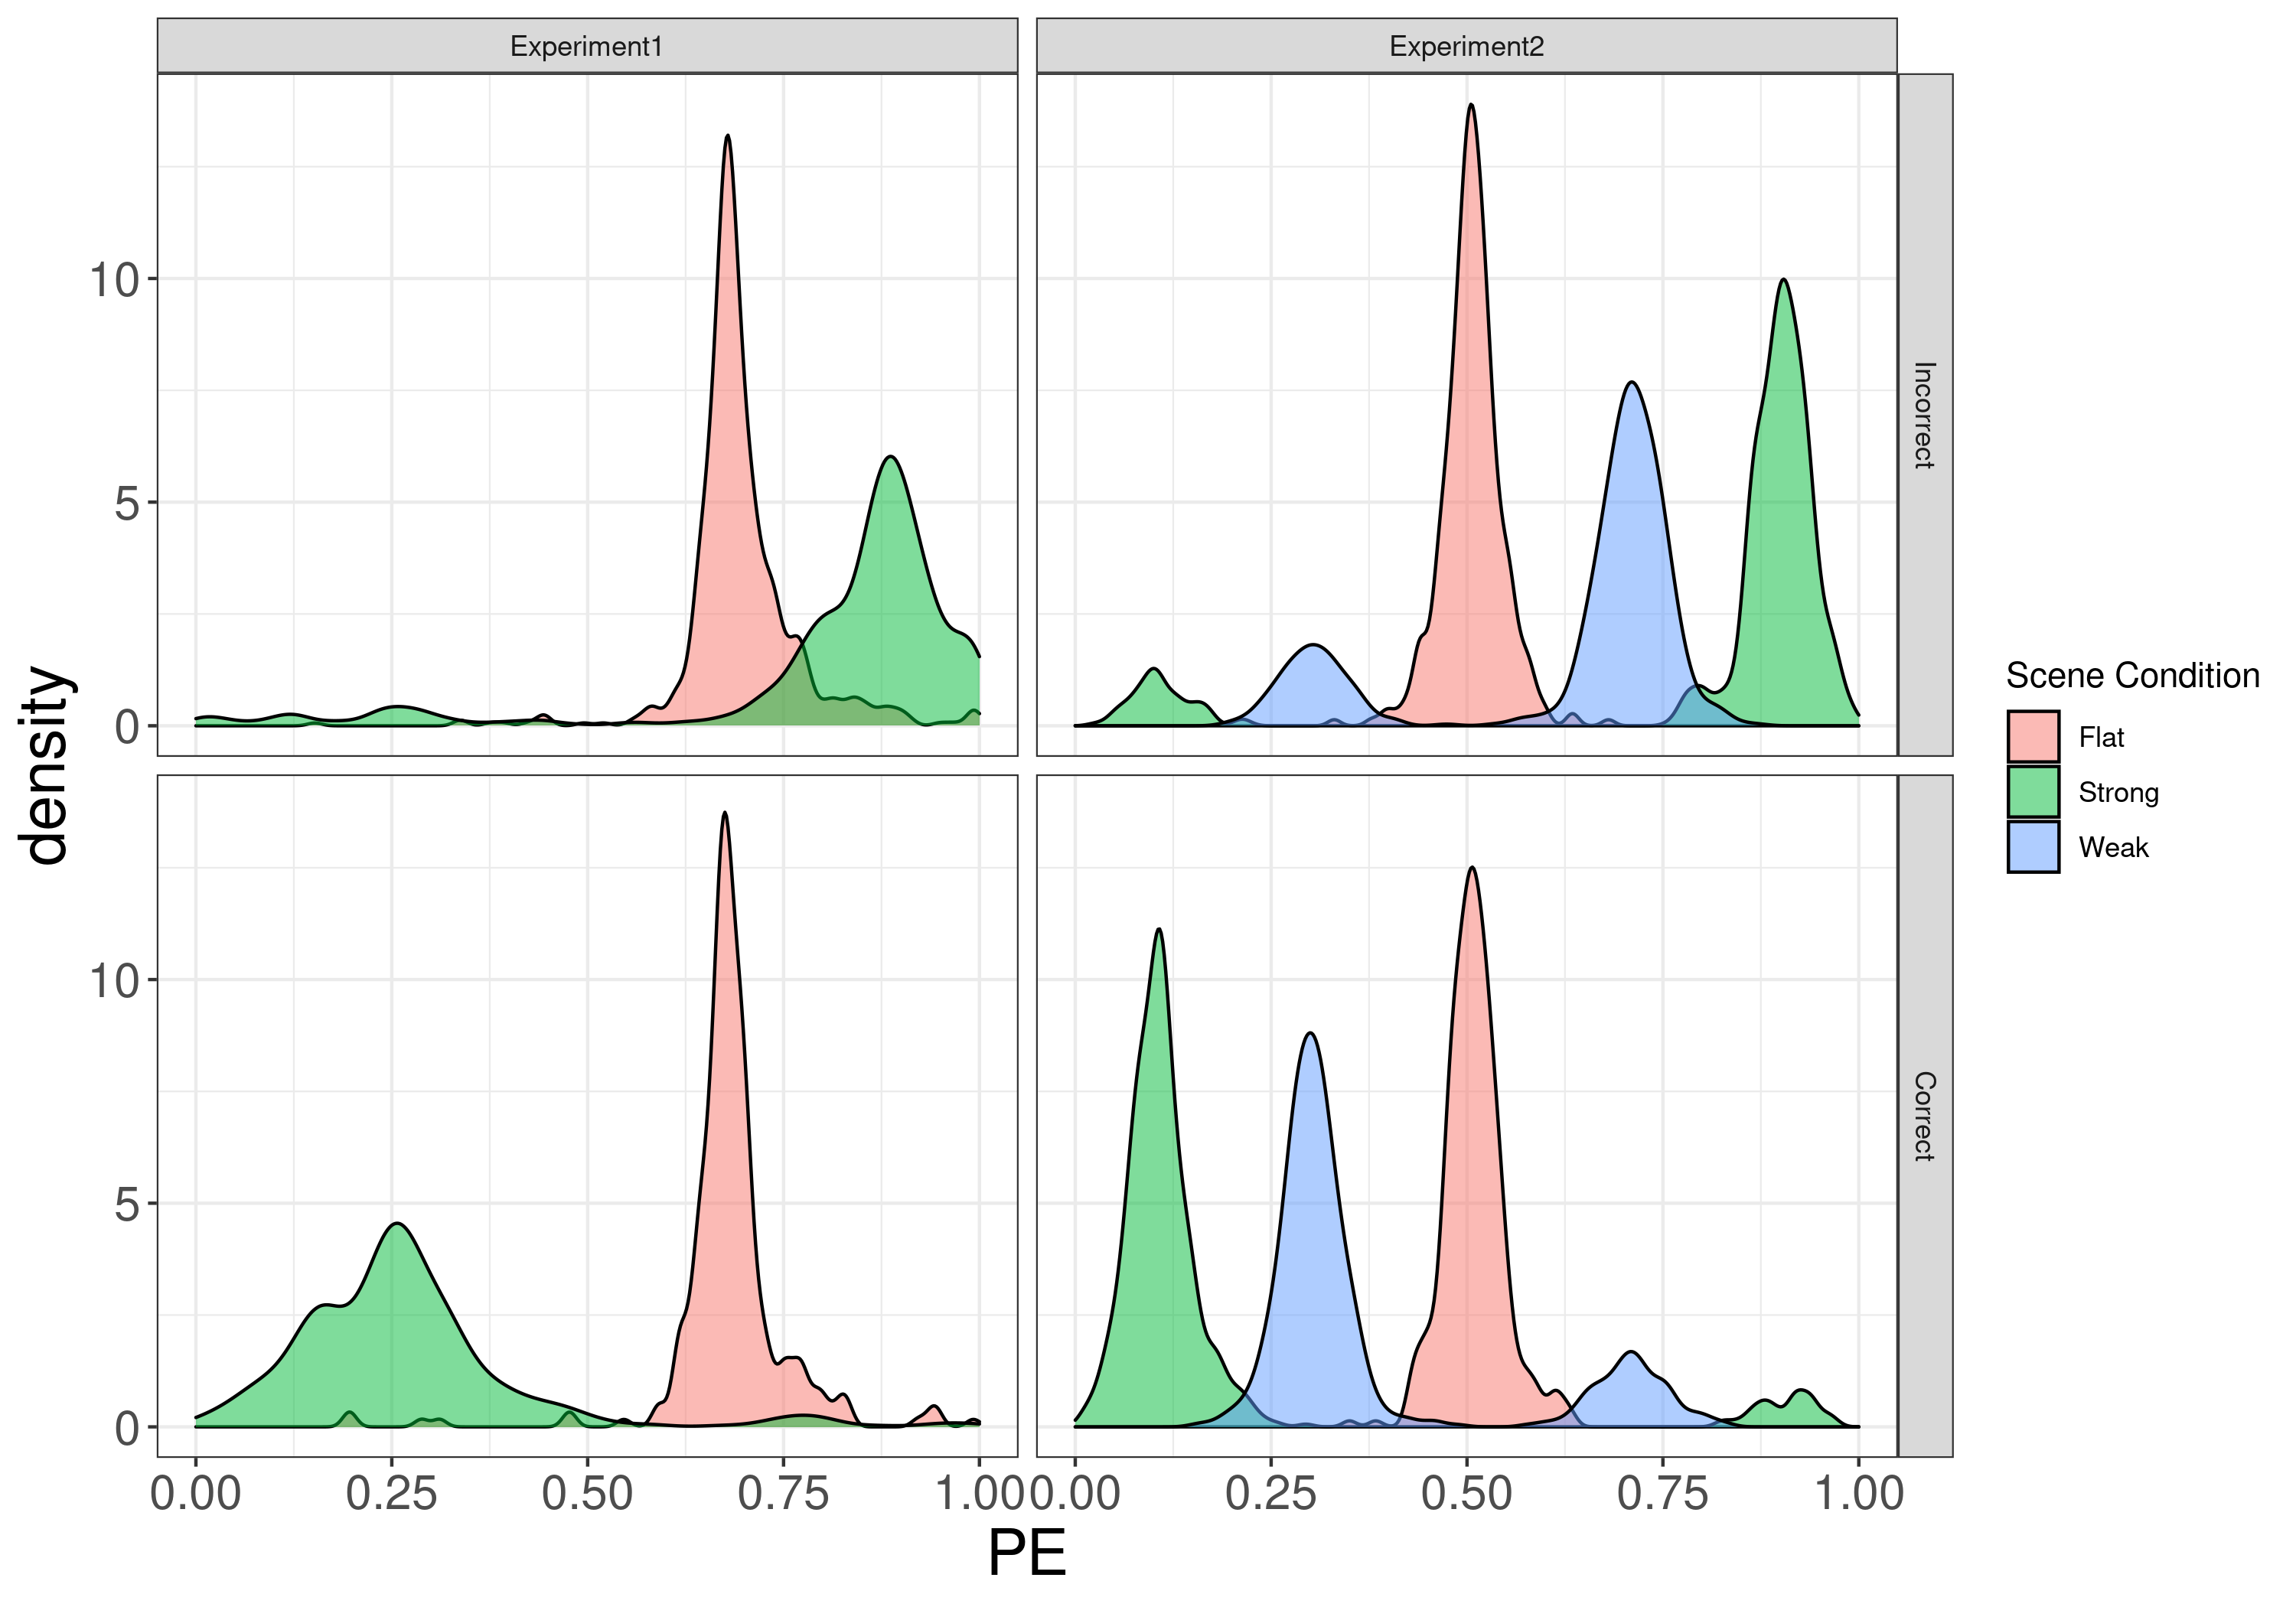
\includegraphics[width=1\textwidth]{figures/PE_byexp_byacc_byscene.png}}\
\caption{\textbf{Distribution of PE as a function of scene condition and prediction accuracy.} Density histograms showing the distribution of PE by scene condition (denoted by the different colors of the histograms), prediction accuracy(incorrect vs correct, indicated by the different rows), and Experiment (indicated by the columns). }
\label{fig:PE_SC:acc}

\end{figure}



\begin{figure}
{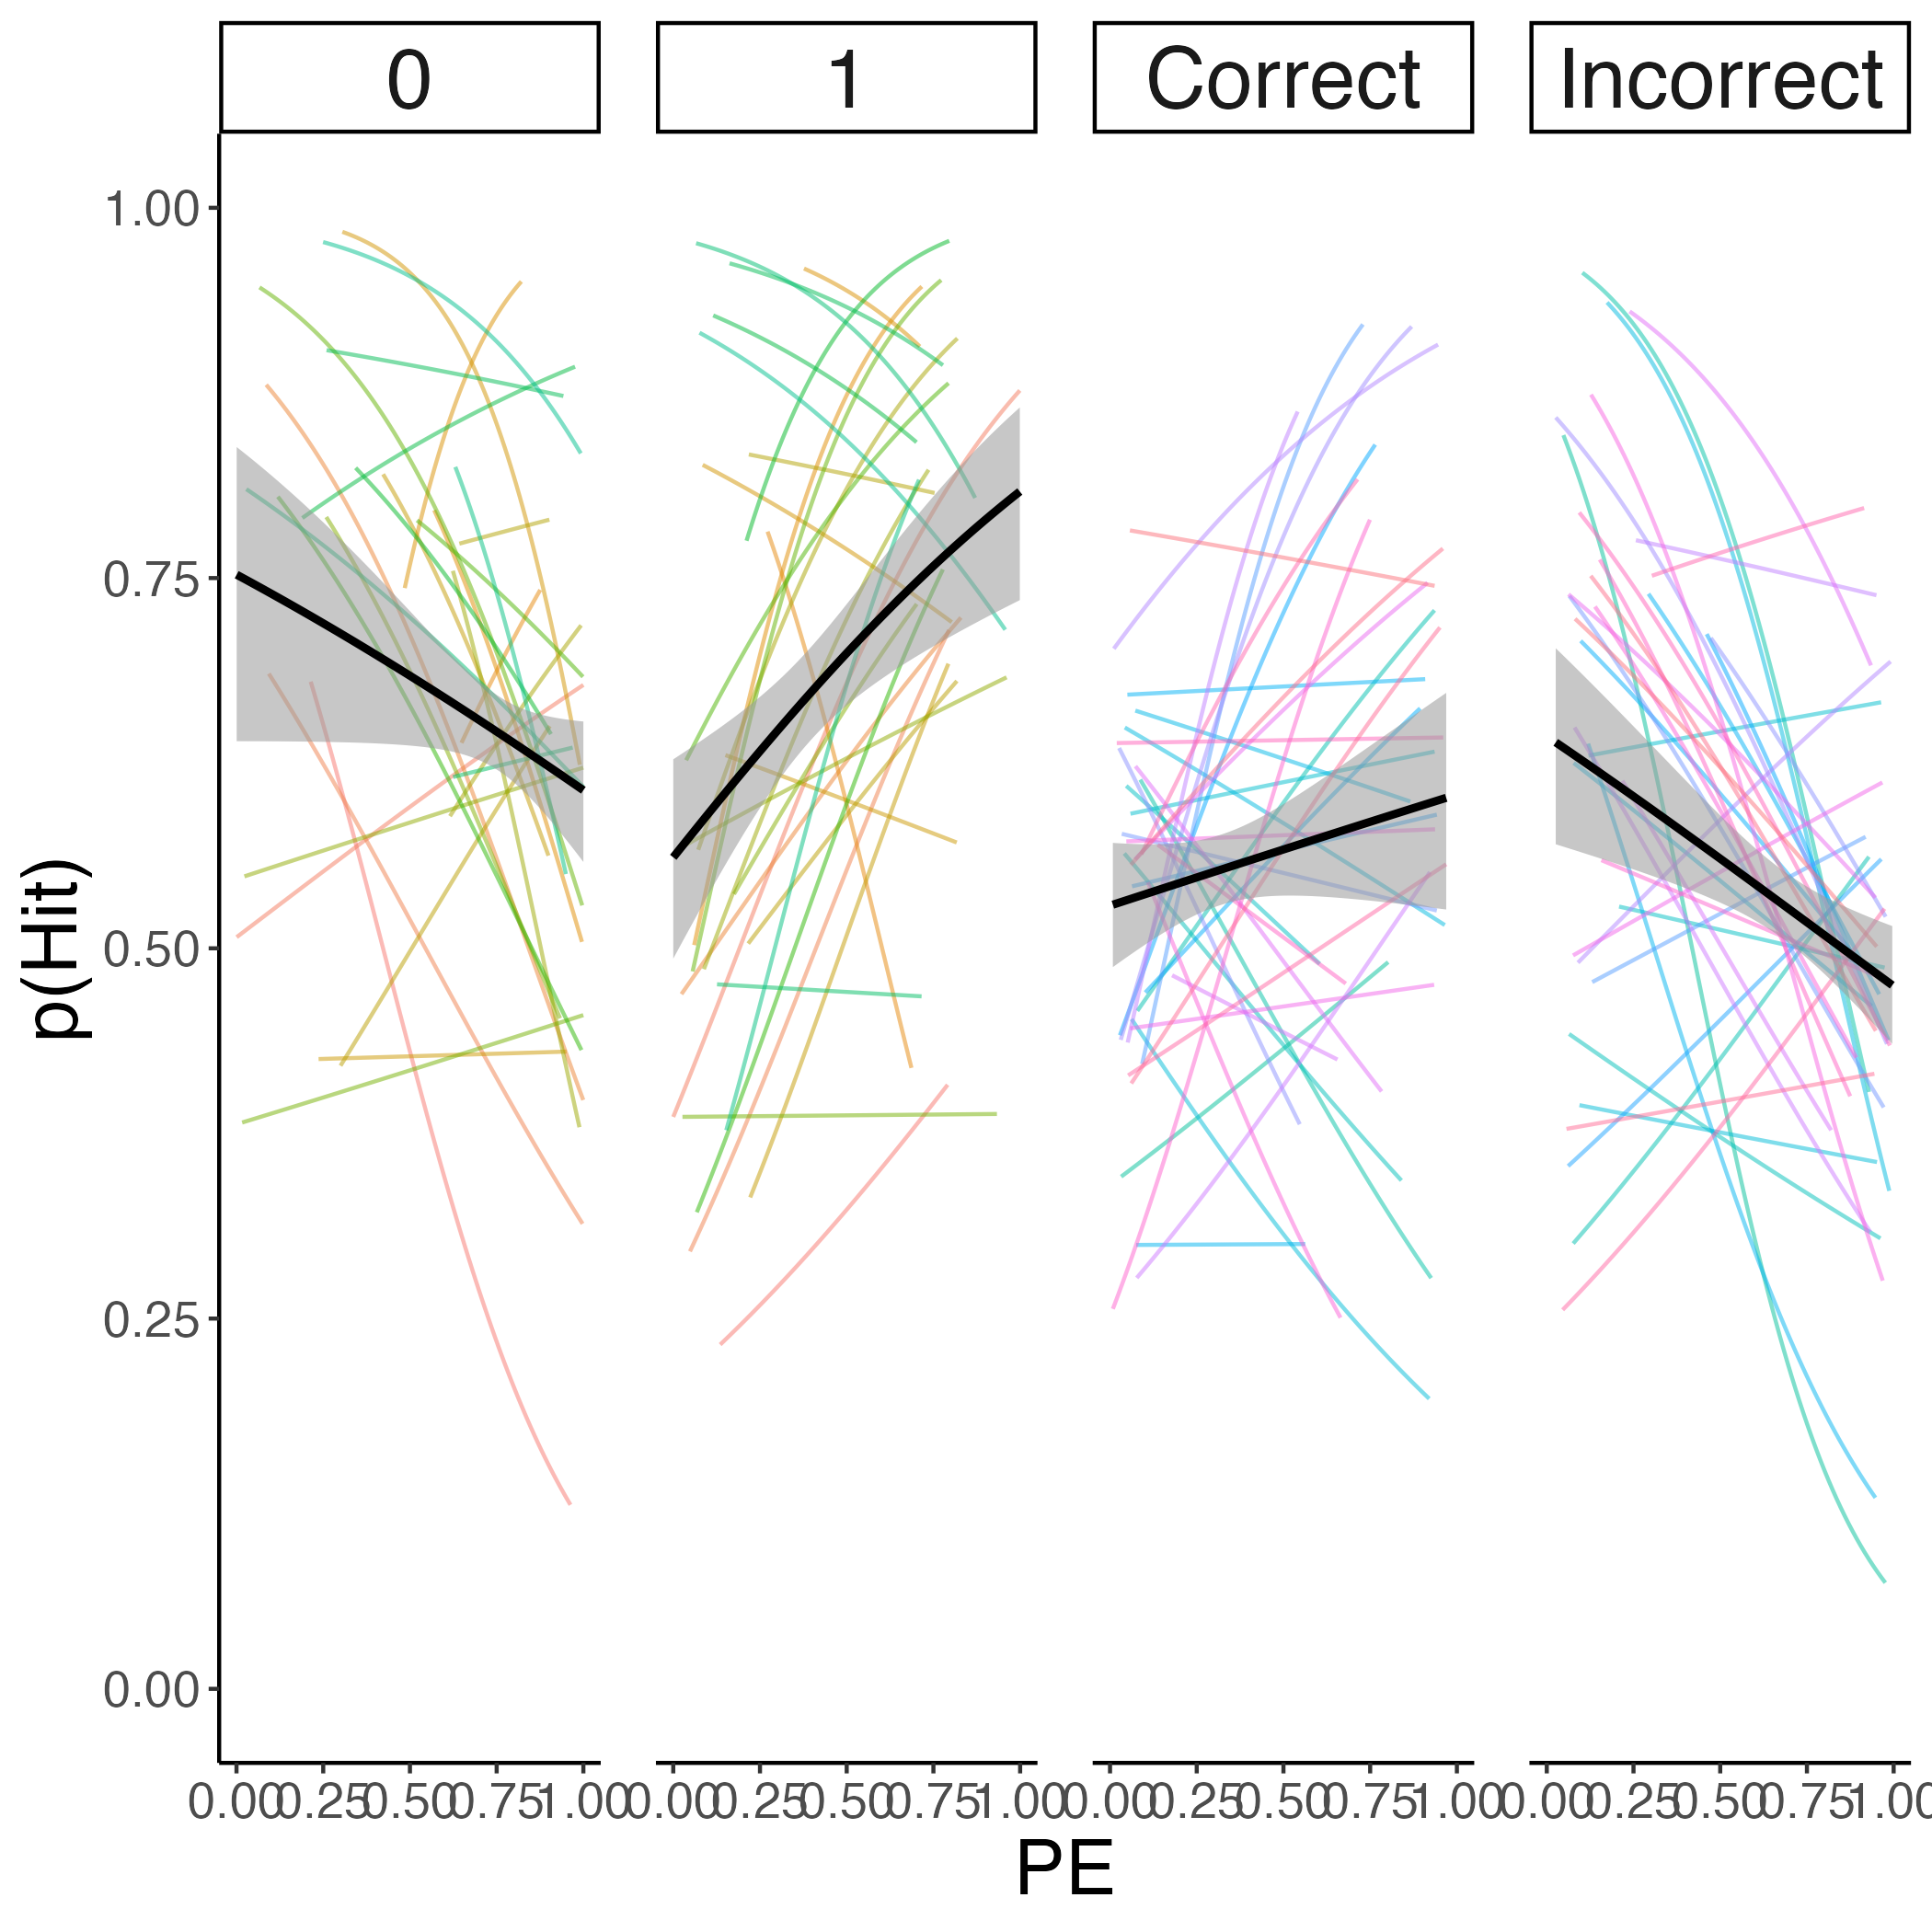
\includegraphics[width=1\textwidth]{figures/PE_mem_fLR_instr.exp1.exp2.png}}\
\caption{\textbf{Observed relationship between PE and recognition memory as a function of prediction outcome for merged data from Experiment 1 and Experiment2.}  }
\label{fig:PE_Mem_1_2}. 

\end{figure}

We tested for the three-way interaction between PE, prediction outcome, and experiment in a generalized linear mixed-effects model, adding participants as random intercept and PE, prediction accuracy, and their interaction as both fixed effect and random slopes. 
The three-way interaction was not significant $\chi^2_{(1)}$ = 1.30, \textit{p} = .253. Moreover, the interactions between PE and experiment, and the interaction between prediction outcome and experiment, were not significant ($\chi^2_{(1)}$ = 0.032, \textit{p} = .858; $\chi^2_{(1)}$ = 0.799, \textit{p} = .371, respectively). These results suggest that effects of PE on recognition memory, and the interaction between PE and prediction outcome, do not change as a function of the experiment. On the contrary, the interaction between PE and prediction outcome was significant, $\chi^2_{(1)}$ = 15.67, \textit{p} < .001. To break down the interaction, the effect of PE on recognition memory was analyzed separately for correct and incorrect prediction outcomes. Results showed a significant positive linear relationship between PE and recognition memory for correct prediction ourcome , $beta$ = 0.80, \textit{p} < .001, OR = 2.22, and a significant negative linear relationship between PE and prediction outcome for incorrect prediction outcome, $beta$ = 0.78, \textit{p} < .001, OR = 0.46.
These results suggest that the strength of the expectations influence memory encoding differently depending on prediction outcome. \par

We ran additional analyses with hit rate binned by aggregating it between the quartiles for PE for each participant. Results from these analyses did not change the overall pattern presented in the previous analyses (see Supplementary Material and Figure \ref{fig:PEbin_mem}). We finally checked whether participants' estimated learning rate, and thus the  degree to which they updated their internal model as a result of a PE, modulated the effect of PE on memory. Coefficients for the interaction between PE and prediction accuracy on memory were extracted for each participant from the generalized linear model and correlated with participant's learning rate. The correlation was not significant,  $r$(59) = .10, \textit{p} = .430, indicating that the overall extent to which participants updated their values was not linked to the interaction between PE and prediction accuracy on memory. We then explored whether participants' learning behaviour in the encoding phase was linked to the the strength of the effect of PE on subsequent recognition. We thus correlated participants' PE-by-prediction outcome interaction coefficients to participants' BIC. The BIC represents how well the model (instructive model with free learning rate) reflected participants' learning behaviour, with lower values indicating better fit. A scatterplot of the relationship is shown in Figure \ref{fig:PE_PE_BIC}.
There was a significant negative correlation between the PE-by-prediction outcome interaction coefficients and the BIC,  $r$(60) = -.33, \textit{p} = .00, indicating that the closer participants' learning behaviour was to the reinforcement learning model, the stronger the PE-by-prediction outcome effect on memory encoding.
 
 \begin{figure}
{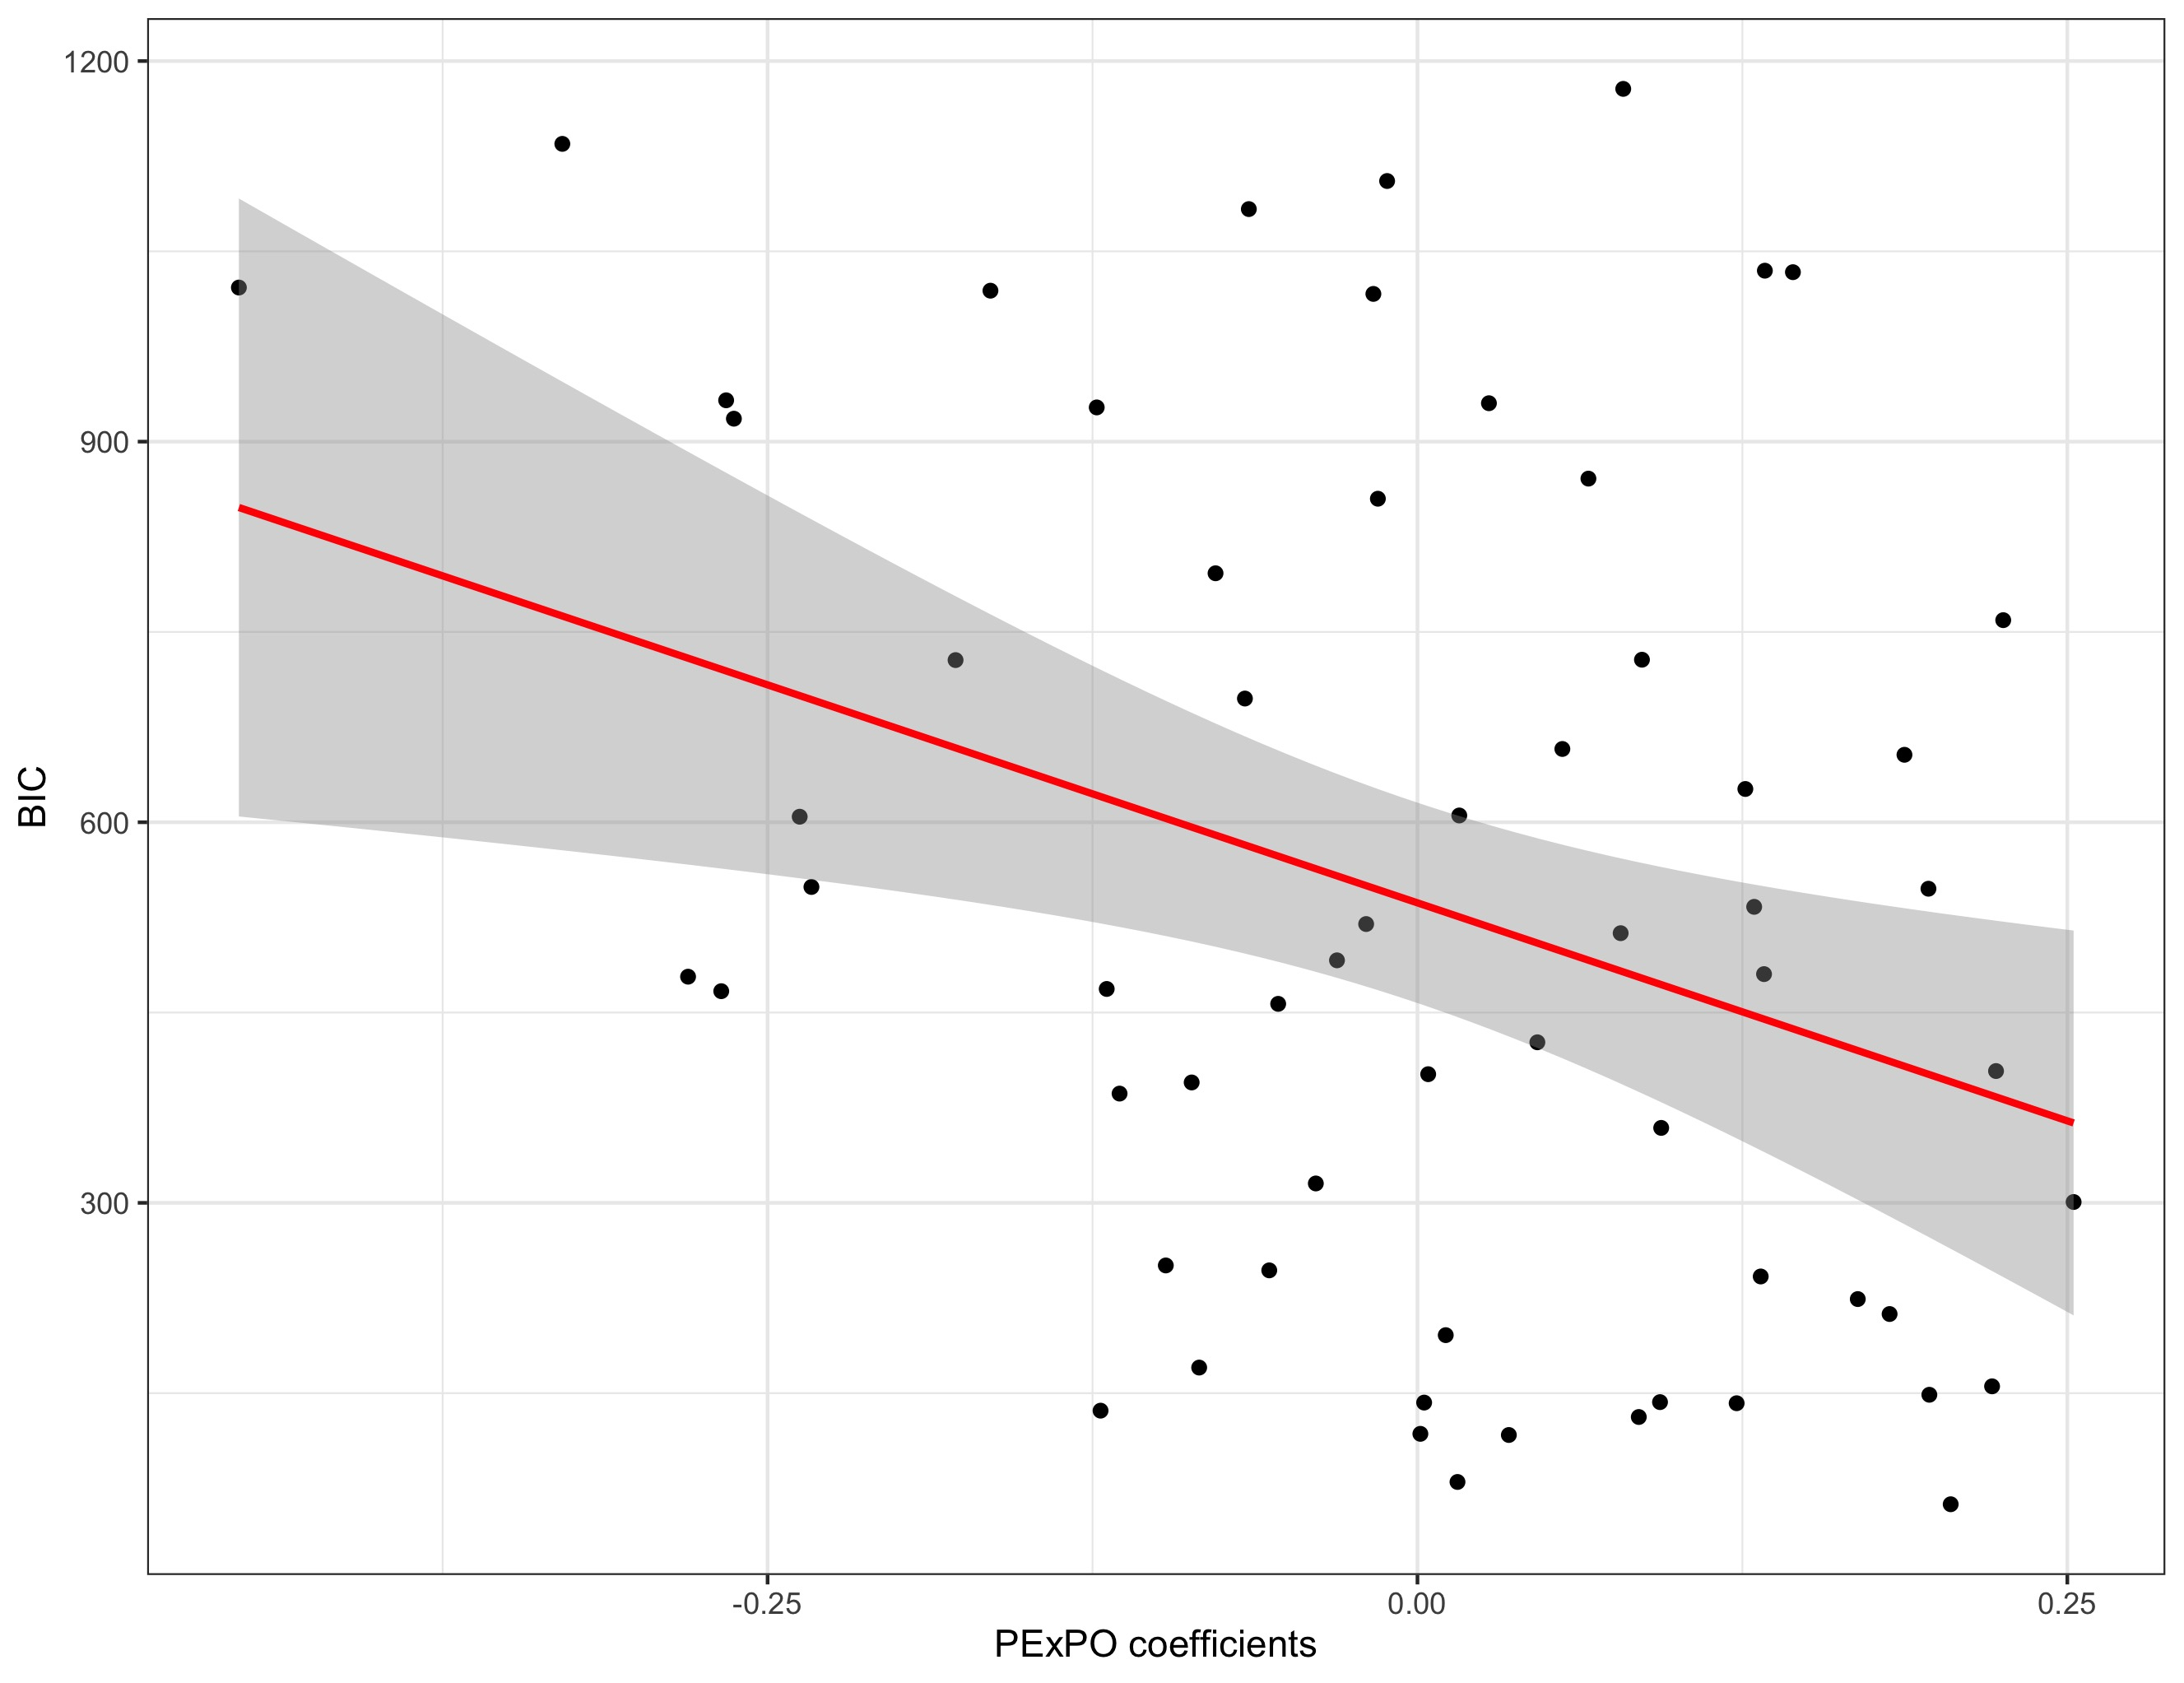
\includegraphics[width=1\textwidth]{figures/PExPO_BIC.jpg}}\
\caption{\textbf{Correlation between PE-by-prediction outcome coefficients and BIC.} Scatterplot showing the relationship between participants' PE-by-prediction outcome interaction effects and participants' BIC. Lower BIC represent better model fit.  }
\label{fig:PE_PE_BIC}

\end{figure}
 
\section{Discussion}
Previous literature has provided mixed evidence on the effects of prior expectations on memory formation \citep{Bein2015, BrodGarvinShingYee2019, Greve2017, Kafkas2018}. Studies on reward PE using reinforcement learning models have also produced contrasting results \citep{Jang2019, de2018signed,Rouhani2018, Rouhani2021}. We explored the effects of PE on memory for the first time in a paradigm which did not included an explicit manipulation of the reward and in conditions in which participants had already established prior expectations. In the task used, associations between context and object categories were first learned by participants and then used to predict the category of trial-unique upcoming objects. In two experiments, we used a reinforcement learning model to derive trial-by-trial PE generated by expectations of different strength and analyzed its effect on memory encoding. We showed that the outcome of participants' predictions was a modulator of the effects of PE on memory encoding. Precisely, when unexpected events were successfully predicted, PE was beneficial to memory encoding; conversely, when expected events were not successfully predicted, PE was detrimental to memory encoding. These results reveal a computationally specific effect of PE, highlighting the crucial modulating role of prediction outcome. \par
Our results showing better memory for events eliciting low PE as a result of correct predictions are in line with studies showing benefits of matching expectations \citep{Bein2015, BrodGarvinShingYee2019, VanKesteren2013}⁠. In fact, findings from the current study reveal that when participants' strong expectations are met, the images presented are remembered better compared to when strong expectations are violated. This effect is driven by the higher PE generated by incorrect predictions in condition of strong expectations, which impairs encoding of the images. However, our results also show that PE can be beneficial to memory in conditions when prior expectations are low and the events are correctly predicted. Situations of weak priors can lead to less confident predictions that benefit from a positive (unexpected) outcome. \par
Our findings are in line with studies on reward PE showing better memory for better than expected outcomes \citep{de2018signed, Jang2019},
a pattern suggested to be related to dopaminergic activity promoting hippocampal plasticity and memory formation \citep{Bethus2010,rosen2015midbrain}. It is well known in computational neuroscience that the neurotransmitter dopamine is responsible for a PE signal that drives plasticity in the striatum, facilitating repetitions of actions with better-than-expected outcomes \citep{Daw2013, Niv2008}. Dopamine is also known to enhance long term potentiation in the hippocampus \citep{lemon2006dopamine}, and this modulatory effect might be responsible for the prioritization of relevant information in memory. \par 
It has also been shown that the effect of dopamine on the hippocampus can be bidirectional: Higher levels of dopamine cause phasic firing in the hippocampus which results in increased activation, while lower levels of dopamine produce tonic firing and inhibit hippocampal activation \citep{rosen2015midbrain}. In the present study, this dopaminergic effect may be driven by the difference between the expectations and the outcome of the prediction. More specifically, a correct prediction in conditions of weak expectations might provide a PE signal that increases the release of dopamine in the striatum, promoting hippocampal activation, and resulting in better encoding. This idea is supported by evidence showing that increased striatum-hippocampus connectivity during learning in some conditions supported enhanced memory encoding \citep{Davidow2016}). Conversely, an incorrect prediction in condition of strong expectations might correspond to a negative PE, which suppress activation in the striatum and in the hippocampus, resulting in impaired encoding. More study investigating the connectivity between hippocampus and striatum at these different conditions are needed to confirm these hypotheses. 
\par 
In the present study, PE is experienced at the time of the presentation of the to-be-remembered items. The object presented provided feedback to participants on whether or not their predictions were correct. Previous studies from De Loof et al. (\citeyear{de2018signed}) and Jang et al. (\citeyear{Jang2019}) found effects of reward PE experienced during item presentation on memory encoding that are consistent with our results. Importantly, the effects found by Jang and colleagues were linked to reward PE elicited at item presentation, but not at the time of the presentation of the feedback, when the objects were no longer shown. This results suggest that the timing of PE relative to image presentation is a key factor for memory effects. 
\par
Results from the current studies are in contrast with previous findings showing effects of unsigned reward PE on memory \citep{Rouhani2018, Rouhani2021}. One possible explanation for this discrepancy is the task that these studies used at encoding. Rouhani and colleagues (\citeyear{Rouhani2018, Rouhani2021}) presented participants with scenes that could be predictive of the future rewards. After participants made their predictions, the images were presented together with the reward received, which could be either better or worse than expected, thus generating a reward PE. In a first study \citep{Rouhani2018}, they showed a positive effect of unsigned prediction error on memory encoding, which thus improved for both better- and worse-than-expected outcomes. However, in this study it was not clear whether the effect was due to PE occurring before or after feedback presentation, as the images were presented even before the presentation of the feedback. In a second study \citep{Rouhani2021}, the authors manipulated reward PE before and during feedback delivery separately, finding an effect of signed reward PE for images presented before feedback delivery and an effect of unsigned reward PE for items presented during feedback presentation. The discrepancy between these finding and our findings can be due to the different methodologies used to elicit PE. In fact, the reward PE experienced during feedback delivery in the study by Rohuani and colleagues \citep{Rouhani2021} was related a precise condition in with participants could win or lose money. As a consequence, the effects observed might have been triggered by arousal-related emotional processes linked to the activity of the amygdala \citep{watanabe2019reward}, which are known to enhance memory  \citep{mather2011arousal}. 

%It is well known that individuals consider differently positive and negative outcomes when updating their beliefs, weighting more positive outcomes than negative ones \citep{Lefebvre2017, sharot2007neural, sharot2016forming}. In addition, a positive outcome associated with a stimulus increases the probability of later remembering it in incidental memory tasks \citep{wittmann2008mesolimbic,mather2011positive, holtje2018electrophysiological}, an effect associated with increased neural activation in the midbrain and the hippocampus \citep{wittmann2005reward}. What is still not clear is whether these effects are scaled by PE. 

 The utility of the information presented may have played a role in the results of the current study. Events can be processed differently depending on whether they are useful to predict events in similar contexts. In fact, while positive feedback when prior expectations are weak may inform individuals that the choice is important for future similar contexts, negative feedback in contexts where prior expectations are strong may inform participants that that event is not useful for future predictions. Therefore, events that are important to guide future behaviour may be remembered better, while those that are deviant from established expectations may be discarded as exceptions. It has been shown that dopaminergic neurons reacts similarly to both rewards and to cues that indicate advance information \cite{ESBromberg-Martin2011}. This effect may reflect in a strengthened representation of items that carry more information for predicting future events, in line with views considering reinforcement learning not only as a reward-seeking system, but also as an information-seeking system \cite{ESBromberg-Martin2011, Niv2011}. More studies are needed to disentangle the effects of reward-seeking and information-seeking processes of PE on memory. \par
 It is important to note that mismatched information might have been discarded as not helpful for the future because the task used in both experiments included contingencies that were established before the encoding of the events and never changed during the course of the tasks.  IParticipants underwent extensive learning phases in which they established their expectations for the different contexts prior to the encoding task. This settings is not frequent in previous computational modeling studies, although it is more common in real life, where in most situations individuals are likely to find themselves in situations they are typically familiar with. In conditions in which expectations are established and known to be stable, deviant information is quite expected. Therefore, it is possible that mismatched information would be more valued during the learning of the priors or in conditions where the environment changes, making the unpredicted outcomes more unexpected. Evidence showing different behavioural and neurophysiological correlates of expected and unexpected uncertainty is in line with this view. \cite{Yu2005}). 
 \par
To characterise the contingency-learning process we fit three different reinforcement learning models to participants' data: An optimal model, a model considering the outcome of participants' choice (evaluative model), and a outcome-free model considering the information given on each trial (instructive model). Model comparison showed that participants' learning processes did not conform to the normative behaviour of a Bayesian model, which prescribes that the optimal way of learning in this task entails decreasing the learning rate proportionally to the inverse of the number of the trials. In fact, participants data were best explained by models estimating individual learning rates. In addition, participants' learning data were best explained by a model in which the context-category associations were learned by increasing the strength of the associations of the category presented on a given trial and decreasing the strength of the associations of the categories not presented, regardless of participants' choice and its outcome. This result suggests that prediction outcome might not be important for PE-driven incremental learning of associations, while it is crucial for modulating the influence of PE on the encoding of item identity. 
In conclusion, the current study provides robust evidence on the effects of PE on memory encoding. We show that the effects of PE on memory are modulated by whether or not a prediction is correct, suggesting a dependency between hippocampal and striatal dopaminergic systems, and informing future studies exploring the interactions between learning and memory. 


\section{Methods}
\subsection{Participants}
In experiment 1, thirty-two young adults (20 female; mean age = 22.59 years, \textit{sd} = 3.18) were recruited through advertisements placed at the Goethe University campi in Frankfurt am Main. In exchange of participation, participants received either course credits or a monetary reimbursement of 8 €/hour. 
In experiment 2, 40 participants (19 female; mean age = 24.87, \textit{sd} = 4.64) were recruited through the Prolific platform https://www.prolific.co/). All participants had normal or corrected-to-normal vision and no history of psychological or neurological disorders. All participants gave written informed consent prior to participation. The study was approved by the ethics committee of the Goethe University Frankfurt am Main. 
\subsection{Materials}
For a more detailed description of the materials and methods used, please refer to the original publication \citep{ortiz2021not}. For experiment 1, six coloured scene categories depicting real world outdoor locations taken from the ECOS database (https://sites.google.com/view/ecosdatabase/) were used as contexts. The selected scene categories were beach, mountain, road, desert, savannah, and seabed. As objects, 192 coloured images depicting real world objects were collected from an online search and were used as target objects. The images selected included the same number of objects for three different object-categories: musical instruments, fruits/vegetables, and household objects. All images were subjected to creative commons licensing and are available at https://github.com/ortiztud/premup. 
For experiment 2, the number and types of the scene categories were the same as experiment 1. By contrasts, the objects categories were reduced and only two were used: musical instruments and household objects. 
\subsection{Design and procedure}
In experiment 1, participants completed the learning, encoding, and retrieval tasks in one session, while in Experiment 2 participants completed the learning phase in a first session and the encoding and retrieval phase approximately 24 hours later. In addition, in the second session of experiment 2 participants worked on an extra reminder block of contingency learning before the encoding phase. 
In Experiment 1, stimulus presentation and recording of the responses was done using MATLAB’s Psychtoolbox (Brainard, n.d.) in a 60 Hz monitor (resolution: 1680 x 1050, full HD). 
 Experiment 2 was moved online due to the COVID-19 pandemic, and some necessary changes were implemented. Stimulus presentation and response collection were programmed in PsychoPy v2021.1.4 and hosted online in Pavlovia (https://pavlovia.org). At the beginning of each session, the experimenter met the participant in a virtual room using an online video-conferencing tool, during which the appropriateness of the testing setup was assessed with a brief set of questions about the participant’s overall well-being, about the physical room in which the task would be performed and about the computer that would be used. Experimenters ensured that all participants were sitting in a quiet room, used a laptop or a desktop computer and were encouraged to minimize distractions as much as possible during the session. At the end of the session, the experimenter met the participant again and ask them about any unforeseen event or situation that might have come up during the completion of the task. Finally, to maximize engagement, self-administered breaks were included after every 40 trials during the contingency learning and the encoding phases. 
\paragraph{Contingency learning phase.}
Participants were presented with the scene contexts on the screen and were instructed to learn which object category was more likely to belong to each of the scene contexts; they were told that some contexts were easier to learn than others, but the exact contingencies were not explicitly given. A fixation cross at the center of the screen marked the beginning of each trial and lasted for 500 ms. After that, a scene image including a rectangular white patch with a question mark was presented. They were then asked to make a prediction about the object category that they thought they would encounter in that context. Three response alternatives were given for Experiment 1 (i.e., musical instruments, fruits/vegetables, and household objects) and only two for Experiment 2 (i.e., musical instruments and household objects). Category reminders were placed at the bottom of the screen and participants could choose among them by pressing one of three arrow keys (left arrow, down arrow, right arrow). The selected category was highlighted with a yellow frame. After 2 seconds from scene onset, the question mark within the white patch was replaced by an objects and the coloured frame changed colour to indicate correct or incorrect response. Specifically, the coloured frame around the image became red to indicate incorrect responses, and green to indicate correct responses. Object and feedback were shown on the screen for 1 second. Participants were told to use the feedback to learn the contingencies over trials. \par
The frequency to which an object category was encountered in the given scene contexts was manipulated to create different prior strengths. The prior strengths were "Flat" and "Strong" in Experiment 1, and "Flat", "Weak", and "Strong" in Experiment 2. In Experiment 1, the "Strong" prior condition consisted on three scene contexts in which one of the three object categories was frequently presented 80 \% of the trials, while the other two were equally presented 10 \% of the trials each. Conversely, the "Flat" prior condition consisted of three scene contexts in which the object categories were all three equally probable, being presented each 33 \% of trials. 
In experiment 2, the "Strong" prior condition was composed by two context scenes where one of the two object categories was presented 90 \% of the trials, while the other object category was presented on 10 \% of the trials. Two more scene contexts belonged to the "Weak" prior condition, in which the more frequently presented object category was shown on 70 \% of the trials, while the other object category appeared on 30 \% of the trials. Finally, the "Flat" prior condition included two scene contexts in which both object categories were equally likely to be presented, appearing each one on 50 \% of the trials. 
In order to achieve the desired contingencies without proportionally increasing the number of individual objects used, different objects were repeated a different number of times depending on its category and on the contexts in which they were shown. The association of each object category to each scene category was counterbalanced across participants so that across the entire sample, every object category was paired with every scene category.
\paragraph{Encoding Phase.}
The encoding Phase in Experiment 1 and 2 was similar to the learning phase, with only minor changes introduced. The explicit feedback represented by the coloured squared surrounding the object was removed in this phase, to avoid its potential effects on episodic encoding. In addition, a new set of objects was used, and each of these objects was presented only once. To equate the number of objects in each critical cell for our analysis, we selected a fixed number of objects (n=20) for each PE condition, and these were presented only once. Then, to achieve the desired contingencies for each scene category, we used filler objects from the same object categories and repeated them 7 times. Filler trials were not considered for recognition memory. \par
Similarly to the contingency learning phase, participants' task was to predict which object category followed a scene context that was presented on every trial. The contingencies between object categories and scenes were the same as the previous learning phase. 
\paragraph{Retrieval Phase.}
In the object recognition test, all the objects from encoding phase together with 192 new objects were used. 
In Experiment 1, hit rate was calculated on a sample of half of the 192 objects (96 trials), as half of the trials were selected for the immediate recognition session which is the object of the analysis of the current study. The rest of the trials were selected for a delayed recognition test, which is not considered in the current study. In experiment 2, all the 192 old objects were considered for hit rate calculation. Trials started with a fixation cross for 500ms, and objects were presented in isolation at the center of the screen. Participants were required to make old/new judgements. All the responses in the retrieval phase were self-paced and not time-constrained, and the display stayed unaltered until participants made a response. After that, a new trial was then presented.

\subsection{Computational Models}
We fitted participants' data with computational models. The models considered are all different version of a standard Rescorla-Wagner model (or Q-learning) \citep{Sutton1998, Daw2011}. For each scene category, the model estimates a trial-level variable \textit{Q} for each object category included in the experiments (three in experiment 1 and two in experiment 2). These \textit{Q} values reflect the strength of participants' belief that a certain object category (for example, "Instruments") will be presented in a specific context (for example, "beach"). 
\noindent
Since we have \textit{N} object categories for each \textit{n} context, the estimates $\hat{Q}$ of the probabilities can be represented by the following \textit{j}-by-\textit{c} matrix:

\begin{equation}
\begin{bmatrix} 
\hat{Q}^{1,1}, & \hat{Q}^{1,2}, & ... \\
\hat{Q}^{2,1}, & \hat{Q}^{2,2}, & ...\\
..., &..., & \hat{Q}^{j,c} \\
\end{bmatrix}
\quad
\label{matrix}
\end{equation}

\noindent
Where $\hat{Q}^{1,1}$ represent the expected value Q for category \textit{j}=1 in context \textit{c}=1. For all the models considered in this study, the estimated values are stored in a category \textit{j} by context \textit{c} matrix as this one, and initialize as  $\hat{Q}^{j,c} = 0.33$ in experiment 1, and $\hat{Q}^{j,c} = 0.5$ in experiment 2.

\paragraph{Decreasing Learning Rate Instructive Model (dLRI)}. First, to provide a normative Bayesian solution, we used a Dirichlet-multinomial model. We applied a multinomial distribution because the categorical distribution that we used in our task is a special case of the multinomial distribution that consists of only one random sample during each trial (see Supplemental Material). The Dirichlet multinomial model can be reformulated to a delta-rule model in which the learning rate constantly decreases inversely proportional to the number of the trial. 
Thus, the delta-rule model sequentially updates the category probabilities for each context according to

\begin{equation}
\hat{Q}_{t+1}^{j,c} = \hat{Q}_{t}^{j,c}  + \dfrac{1}{t} \delta_{t},
\end{equation}


\noindent
where $\hat{Q}_{t+1}^{j,c}$ denotes the estimate of the probability of category $j$ in context ${c,j}$ at the next trial $t+1$. This estimate is based on the current estimate of the category probabilities ($\hat{Q}_{t,j}^{j, c}$) and the prediction error $\delta$, calculated as:

\begin{equation}
{\delta} = {r}_t^{j} - \hat{Q}_{t}^{j,c}
\label{eq:PE}
\end{equation}

\noindent
where the feedback ${r}_t^{j}$ represents an array of \textit{N-by-j} elements, in which each element refers to a category \textit{j}, defined as following:

\begin{equation}
r_t^j = \begin{cases}
1\ if  \ j = j_t  \\ 
0 \ otherwise
\end{cases}
\label{eq:instrPE}
\end{equation}

\noindent
 The values of the array are 1 if category \textit{j} is present on trial \textit{n}, and 0 if it is not. Therefore the model is assuming that a value estimate for an object category that appears on a trial incrementally increases as a result of a prediction error until $Q_{t}^{j,c}$ reaches its asymptote of 1. Conversely, the value estimates of categories that are not presented on trial \textit{t} decrease as a results of a negative prediction error, unless $Q_{t}^{j,c}$ for those categories has already a value of 0. 
Therefore, this model only uses instructive feedback, which indicates what is the correct choice, independently of participants' action. The learning rate $1/t =: \alpha$ indicates to which degree the prediction error influences the updated estimate of the category probabilities. Given that the learning rate in our case directly depends of the number of completed trials $t$ for a context \textit{c}, it continuously decays as a function of trials. This principle ensures that the influence of prediction errors is stronger at the beginning of the task. For more information about the formalization of the optimal Bayesian model, see Supplemental Material. 

\paragraph{Free Learning Rate Instructive Model (fLRI)}. The dLRI shows how an optimal agent should update the expected values. However, participants' behaviour may be far from optimal. %citation needed 
For this reason, the fLRI allows each participant to have its own learning rate $\alpha$. The expected values are thus updated according to the following rule: 

\begin{equation}
{Q}_{t+1}^{j,c} = {Q}_{t}^{j,c}  + {\alpha} \delta_{t},
\label{eq:fLRI}
\end{equation}

\noindent
while $\delta$ is the same as in equation \ref{eq:PE}. Also, note that this model uses the same instructive feedback as in equation \ref{eq:instrPE}.

\paragraph{Free Learning Rate Evaluative Model (fLRE)}. This model still allows participants to have a fixed learning rate $\alpha$. However, this model assumes that the feedback depends on the actions that participants take. The expected values are thus updated as follows:


\begin{equation}
{Q}_{t+1}^{j,c} = \begin{cases}
{\alpha} \delta_{t}\ if  \ a_t = j_t \  \\ 
{Q}_{t} \ otherwise
\end{cases}
\end{equation}

\noindent
where $a_t$ is the object-category selected by participants on a given trial, $\delta_{t}$ is calculated as in equation \ref{eq:PE}, and $r_t$ is 1 if the choice is the correct one, and 0 otherwise. 

\subsubsection{Action Selection} The expected \textit{Q}-values computed through the models listed above were translated into choice probabilities by implementing a softmax rule as follows: 

\begin{equation}
P_t^{j,c} = \dfrac{ exp({\beta} {Q}_t^{j,c})   }
{ \sum_{j=1}^j (exp({\beta} {Q}_t^c) },  
\end{equation}

\noindent
where $P_t^{j,c}$ represents the probability of choosing a specific object-category \textit{j} for a defined scene category \textit{c}. The inverse temperature parameter $\beta$ is another free parameter that modulates the stochasticity of the choice, with higher values meaning more deterministic actions and lower values more noise-sensitive choices. 

\subsubsection{Parameter Recovery} Before fitting the models to participants' data, a parameter recovery procedure was run for both Experiment 1 and Experiment 2, in order to check whether the fitting procedure for each model gave meaningful parameters and to find potential parameters boundaries. \textit{Surrogate} data with randomly sampled known parameters where simulated, then the models were fit to the simulated data \citep[see][]{Wilson2019a}. The priors from which the simulation parameters were sampled are shown in table \ref{tab:priors}. In order to fit the data, we used maximum likelihood estimation (see section). Because the models are designed to reflect participants' learning, only the strong (Experiment 1) and strong and weak (Experiment 2) conditions were simulated. High correlation between simulated and fitted data indicates that the model successfully recovered the parameters that were used to generate the data. First attempts to recover the parameters allowed to set the boundaries for inverse temperature parameters. Plots of the parameter recovery are shown in figure \ref{fig:parameter_recovery}.

% The alpha parameter, the learning rate, was drawn from a uniform distribution (min=0, max =1). The beta parameter, the inverse temperature parameter, from drawn from an exponential distribution. Beta parameter was constrained at 30 after inspection of the first parameter recovery plots, as for values that are above that boundary parameter do not affect behavior much (Wilson and Collins, 2019). Stickiness parameter is drawn from normal distribution with mean 0 and sd 1.



\begin{table} 
    \centering 
    \caption{Priors for the parameters}
    \scalebox{1}{
    \begin{tabular}{l l}
     \hline
    Parameter & Priors \\
    \hline
    
 ${\alpha}$ & $\sim U(0,1)$ \\
  ${\beta}$ & $\sim exp(1)$ \\
     \hline
    \end{tabular}
}
    \label{tab:priors}
    \end{table}



\subsubsection{Model Recovery}
Besides parameter recovery, another procedure to evaluate the reliability of the model is model recovery \citep{Wilson2019a}. The aim of model recovery is to determine that a model, among several ones, can successfully be indicated to be the one to have generated the data. To achieve this, data of the three different models were simulated (with randomly sampled parameters) and then fit to each of the models. The models were then compared to determine which one fitted the data best. The method used to assess the fit of the models was the Bayesian Information Criterion, \textit{BIC}, which incorporates a penalty for the number of parameters:

\begin{equation}
BIC = {-2}log \hat{LL} + k_m log{(T)},
\label{eq:BIC}
\end{equation}

\noindent
where $\hat{LL}$ is the log-likelihood value when the model is fitted with the best fitting parameter, and $K_m$ is the number of parameters in the model \textit{m}. Lower values of \textit{BIC} mean better fit. The comparison between the models for each set of generated data was repeated 100 times to generate the confusion matrices shown in figure \ref{fig:model_recovery}.



% To capture the influence of the learned category probabilities on memory consolidation, we need a model that accurately establishes contextual priors during the learning phase. As shown in Section \ref{dmn} and \ref{delta} in the Appendix (Section \ref{apppendix}), k. In Figure \ref{fig:phase_1_strong}, we provide an example of the delta rule model for categories with $\boldsymbol{\theta}=(0.8,0.1,0.1)$ and \hl{$N=24$} trials. The first row of plots shows the sampled categories across the trials. The second row of plots shows the corresponding prediction errors. For instance, at the first trial the model did expect each category with probability $\boldsymbol{\hat{\theta}}=(0,0,0)$ and observed category 1. In response to this, the model computed a prediction error $\delta_{1,1}=1$ and for the other categories $\delta_{1,2}=0$ and $\delta_{1,3}=0$. Finally, the last row of plots shows the evolution of the expected values that are updated in response to the prediction error. Figure \ref{fig:phase_1_flat} shows an example of the flat prior condition ($\boldsymbol{\theta}=0.33,0.33,0.33$). Obviously, the frequency with whichttps://www.overleaf.com/project/6040f176de7d0939c7e879efh the categories are presented is more similar compared to the strong prior condition, which is reflected in the model's learned expected value that converges to $\hat{\theta}_{n,j(c_n)} = 0.33$ for all categories.

\subsection{Parameter Estimation and Model Comparison}
The models where finally fit to participants' data in order to estimate the parameters. The parameters of best fit for each model were estimated through maximum likelihood estimation. This procedure allowed to find the parameters $\theta$ that maximize the likelihood of the data given the parameters $p(d_{1:t} | \theta, m )$. 
The probability of the whole dataset \textit{d} is calculated as the product of the choice probabilities $p(c_t | d_{1:t-1}, \theta, m)$. As the product of the choice probabilities is often a very small number, it is common practice to use the log-likelihood instead, which is the sum of the log of the choice probabilities \cite{Daw2011, Wilson2019a}:

\begin{equation}
LL = \sum_{t=1}^{n} \log{p(c_t | d_{1:t-1} , \theta, m)}
\end{equation}

\noindent
where $p(c_t | d_{1:t-1}, \theta, m)$ is the probability of each single choice given the parameter $\theta$, the model \textit{m}, and all the data up to that point. \par
The search over the full set of free parameters was optimized through the package \textit{optim} in R, which was fed with the negative log likelihood and a set of starting points randomly selected from the priors shown in Table \ref{tab:priors}. The $\alpha$ parameter was constraint between 0 and 1, while the $\beta$ parameter between 0 a and 10, as parameter recovery shown that for values that exceeded 10 the model could not distinguish between different beta parameters. Because the optimizer may find a local rather than a global, we run the search for the best parameters five times, starting from different points, and then used the best winning parameters among the five iterations, i.e. the parameters that minimized the log-likelihood. 
After estimating the parameters, a \textit{BIC} value(see equation \ref{eq:BIC}) was computed for each model and for each participant using the parameters of best fit. \par
To compare the fit of the models, we calculated the average \textit{BIC} across all subjects for each model, then counted the number of participants for which each model was the best fit. In addition, we used the model evidence of the best model within each participant: Following \cite{raftery1995bayesian} and \cite{gluth2017attraction}, model evidence was defined as "weak", "positive", "strong", or "very strong" depending on the \textit{BIC} difference between the best and the second best model for each participant. Precisely, evidence was "weak" when the \textit{BIC} difference between best and second best model was below 2, "positive" when it was between 2 and 6, "strong" when it was between 6 and 10, and "very strong" when it was above 10. 

\subsection{Statistical Analysis}
In order to test the statistical significance of the effects of interest, we used linear mixed-effect models and generalized linear mixed-effect models, implemented in R through the package \textit{lme4} \citep{bates2014fitting}. Because our main outcome variable (memory) is binary, we used the logit link function in the binomial family to fit the models to accuracy data. Participants were modelled as random intercepts, while the explanatory variables and their interactions were modelled as both fixed and random effects. The resulting generalized linear-mixed effect model can be formalized as the following:

\begin{equation}
p(Hit)_{i,j} =   \dfrac{1}{1+exp - (\beta_{0,j} +\beta_{1_j} PE +\beta_{2_j} PO + \beta_{3_j} PE \cdot PO + \epsilon_{i,j} )}.
\end{equation}

\noindent
The formula represents the probability of remembering an object \textit{i} for a participant \textit{j}. The intercept $\beta_{0,j}$ is composed by a common (fixed) intercept for the population (i.e. the average $p(Hit)$) plus a subject-specific random effect. $\beta_{1,j}$ PE and $\beta_{2, j}$PO represent the slopes for PE and prediction outcome, respectively, while  $\beta_{3, j} PE \cdot PO$  refers to their interaction. Each of slope coefficients is formed by a common (fixed) slope for the population level plus a subject-specific random slope. Finally, $\epsilon_{i,j}$ represents the within-participant residual term.
The variance-covariance matrix for the random effects was set as unstructured, so that the covariances between the random terms could take any finite positive value.  Therefore, we used the maximal random effect structure justified by the design \citep{barr2013random}. The test of the significance of the parameters was obtained through Wald chi-square test. Effect sizes were reported as exp($\beta$), which represent odds ratio, which represents the change in odds. The odds are in turn calculated as follows:

\begin{equation}
Odds =   \dfrac{p(Hit=1)}{1-p(hit=1)}
\end{equation}

\noindent
In the analysis of the effect of binned PE, we used a linear mixed-effect model, with hit rate as response variable:

\begin{equation}
Hit Rate =   \dfrac{hits}{hits+missed}.
\end{equation}

\noindent
Binned PE was treated as a categorical variable with four levels. Testing for significance of planned contrasts was corrected for multiple comparison by using Bonferroni correction:

\begin{equation}
p_{corr} =   p \cdot k, 
\end{equation}

\noindent
where\textit{p} is the \textit{p} value of the comparison and \textit{k} is the overall number of comparisons considered in a model. 




\bibliographystyle{apalike}
\bibliography{library} 

%%%%%%%%%% Merge with supplemental materials %%%%%%%%%%
\pagebreak
%\widetext
\begin{center}
\textbf{\large Supplemental Materials}
\end{center}
%%%%%%%%%% Merge with supplemental materials %%%%%%%%%%
%%%%%%%%%% Prefix a "S" to all equations, figures, tables and reset the counter %%%%%%%%%%
\setcounter{equation}{0}
\setcounter{figure}{0}
\setcounter{table}{0}
\setcounter{page}{1}
\makeatletter
\renewcommand{\theequation}{S\arabic{equation}}
\renewcommand{\thefigure}{S\arabic{figure}}
\renewcommand{\bibnumfmt}[1]{[S#1]}
\renewcommand{\citenumfont}[1]{S#1}

%%%%%%%%%% Prefix a "S" to all equations, figures, tables and reset the counter %%%%%%%%%%
\section{Supplemental Material}
\subsection*{Dirichlet-multinomial model}
We will start with an application of the Dirichlet-multinomial model to all $N$ trials of the learning phase. We apply the Multinomial distribution because the Categorical distribution that we use in our task is a special case of the Multinomial distribution that consists of only one random sample during each trial (see ''Multinomial distribution'' in the Appendix). The Dirichlet distribution is the conjugate distribution of the Multinomial distribution and can therefore be utilized as a prior. 

\paragraph{Likelihood}
After the observation of $N$ pictures during the learning phase, the likelihood of the data $\boldsymbol{\mathcal{D}}=\{x_1,...x_N\}$, where $x_i \in \{1,...,K\},$ can be denoted as

\begin{equation}
p(\boldsymbol{\mathcal{D}}|\boldsymbol{\theta})= \prod^K_{k=1}\theta^{N_k}_k 
\end{equation}

where $N_k = \sum_{i=1}^{N}\mathbb{I}(y_i=k)$. Intuitively, $\boldsymbol{\mathcal{D}}$ denotes the observed data with each $x_i$ indicating how often each category was shown during the learning phase. Please note the similarity to the Categorical distribution that was introduced in ''Formal description of the task''. The major difference is that we now consider all trials of the learning phase.

\paragraph{Prior}
The prior is the Dirichlet distribution
\begin{equation}
\begin{aligned}
p(\boldsymbol{\theta}) & = \mathrm{Dir}(\boldsymbol{\theta}|\boldsymbol{\alpha})\\
&\triangleq \dfrac{1}{B(\boldsymbol{\alpha})} \prod^K_{k=1}\theta_k^{\alpha_{k-1}}\mathbb{I}(\mathrm{x}\in S_K).	
\end{aligned}
\end{equation}
In our case, the Dirichlet distribution is used to model our prior expectations (i.e., at the beginning of the learning phase) about the category probabilities, which is often referred to as pseudo-counts. The parameter that reflects our prior is denoted by $\boldsymbol{\alpha}$. It is fair to assume that participants start the task with a flat prior that reflects that all categories are equally likely, which corresponds to $\boldsymbol{\alpha} = (1,1,...,1)$. These values thus indicate the assumption that each category has been pseudo-counted once. For a few more details about the Dirichlet distribution see ''Dirichlet distribution'' in the Appendix and \cite{Murphy2012}.

\paragraph{Posterior}
The posterior is a Dirichlet distribution that results from multiplying the likelihood by the prior

\begin{equation}
\begin{aligned}
p(\boldsymbol{\theta}|\boldsymbol{\mathcal{D}})
&\propto p(\boldsymbol{\mathcal{D}}|\boldsymbol{\theta})p(\boldsymbol{\theta})\\
&\propto \prod^K_{k=1} \theta^{N_k}_k \theta_k^{a_{k}-1} \\
&= \prod^K_{k=1} \theta^{\alpha_k+N_{k}-1}_k \\ 
&= \mathrm{Dir}(\boldsymbol{\theta}|\alpha_1 + N_1,...,\alpha_K + N_K).
\end{aligned}
\end{equation}
The only operation that is required here is thus the addition of the observed data to the prior. This affords a simple application of the model without the need for complex computations.

\paragraph{Maximum a posteriori and maximum likelihood estimate}
In order to obtain an estimate of the category probabilities, we can compute the expected value of the posterior to obtain the maximum a posteriori (MAP) estimate:
\begin{equation}
\hat{\theta}_k = \dfrac{N_k+\alpha_k-1}{N+\alpha_0-K}.
\end{equation}
Under the assumption that $\boldsymbol{\alpha} = (1,1,...,1)$, the MAP estimate is equal to the maximum likelihood (ML) estimate that is based on the empirically observed frequency of the categories:
\begin{equation}
\hat{\theta}_k = \dfrac{N_k}{N}.
\label{eq:dmm}
\end{equation}
We already noted that in this simple version of the task, we are only required to count our observed categories. Now we additionally know that the category probabilities can simply be obtained by computing the empirical fraction of the number of times each category was presented. This affords a straightforward reformulation of our Dirichlet-multinomial model into an iterative prediction error correcting scheme.


\subsection{Delta-rule formulation}\label{delta}

We now show how eq. \ref{eq:dmm} can be translated into the delta rule. Let $\hat{\theta}_{n,j}$ denote the estimate of the $j$th category probability at trial $n$, then the estimate of the $j$th category at trial $n+1$, denoted by $\hat{\theta}_{n+1,j}$, can be computed according to 


\begin{equation}
\begin{aligned}
\hat{\theta}_{n+1,j} &= \dfrac{n_{j}}{n} \\ 
&= \dfrac{1}{n}n_{j} \\ 
&= \dfrac{1}{n}\sum_{i=1}^{n}x_{i,j} \\
&= \dfrac{1}{n}\Big(x_{n,j} + \sum_{i=1}^{n-1}x_{i,j}  \Big) \\
&= \dfrac{1}{n}\Big(x_{n,j} + (n-1)\hat{\theta}_{n,k} \Big) \\
&= \dfrac{1}{n}\big(x_{n,j}+n\hat{\theta}_{n,j}-\hat{\theta}_{n,j}\big) \\
&= \hat{\theta}_{n,j} + \dfrac{1}{n}(x_{n,j} - \hat{\theta}_{n,j}),
\end{aligned}
\label{eq:model}
\end{equation}
where $(x_{n,j}-\hat{\theta}_{n,j}) =: \delta_{n,k}$ corresponds to the prediction error and the learning rate is defined as $\dfrac{1}{n}=:\alpha_{n,j}$ \citep{Sutton1998}.

\subsection*{Dirichlet distribution}

\paragraph*{Probability simplex}

\begin{equation}
S_K = \{\mathbf{x} : 0\le x_k \le 1, \sum^K_{k=1}x_k=1\}
\end{equation}

\paragraph*{Probability density function}

\begin{equation}
\mathrm{Dir}(\boldsymbol{\mathrm{x}}|\boldsymbol{\alpha}) \triangleq \dfrac{1}{B(\mathbf{\boldsymbol\alpha})} \prod^K_{k=1}x_k^{\alpha_{k-1}}\mathbb{I}(\boldsymbol{\mathrm{x}}\in S_K)	
\end{equation}

where

\begin{equation}
B(\boldsymbol{\alpha}) \triangleq \dfrac{\prod_{k=1}^K \Gamma(\alpha_k)}{\Gamma(\alpha_0)} 	
\end{equation}

and where


\begin{equation}
\alpha_0 \triangleq \sum_{k=1}^K\alpha_k.
\end{equation}


\subsection*{Multinomial distribution}

Let $\boldsymbol{\mathrm{x}}=(x_1...x_K)$ be a random vector, where $x_j$ denotes the number of times picture $j$ in the current context occurs.

\paragraph*{Probability mass function}

\begin{equation}
\mathrm{Mu}(\boldsymbol{\mathrm{x}}|n,\boldsymbol{\theta}) \triangleq \binom{n}{x_1...x_k} \prod^{K}_{j=1}\theta_j^{x_j}
\end{equation}
where

\begin{equation}
 \binom{n}{x_1...x_k}\triangleq\dfrac{n!}{x_1!x_2!...x_3!}.
\end{equation}
In case of $n=1$:

\begin{equation}
\mathrm{Mu}(\boldsymbol{\mathrm{x}}|1,\mathbf{\theta})= \mathrm{Cat}(x|\boldsymbol{\theta})\triangleq \prod^K_{j=1}\theta^{\bold{I}(x_j=1)}
\end{equation}

%\bibliographystyle{apalike}
%\bibliography{library} 

%\bibliographySM{library}

\subsection*{Parameter Recovery}
In order to check whether the models could successfully recover the parameters, \textit{fake} data were first simulated with known parameters. Next, models were fit to the simulated data and parameters of best fit were estimated. Finally, the recovered parameters were compared with the known parameters. Graphs showing the results of parameter recovery are presented in Figure \ref{fig:parameter_recovery}. High correlation between the simulated and fitter parameters indicates successful recovery. Note that the inverse temperature parameter was constraint between 0 and 10 as previous parameter recovery attempts showed that recovery was not reliable for parameters above that range. 


\begin{figure}[ht!]
\centerline
{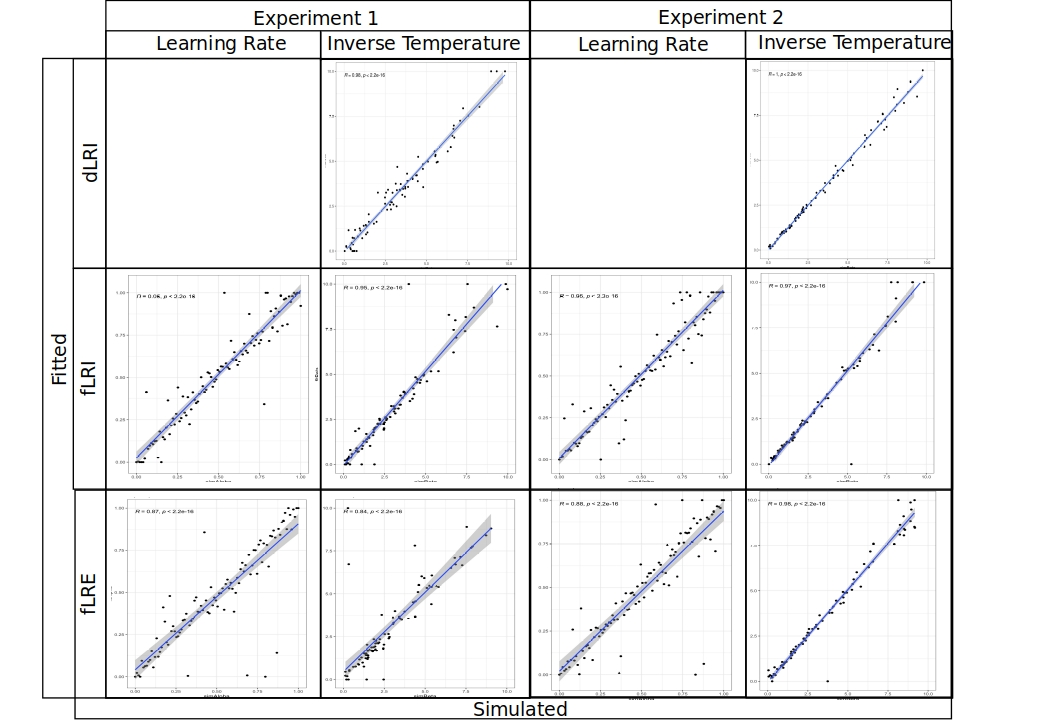
\includegraphics[width=1.5\textwidth]{figures/ParameterRecoveryAll.jpg}}
\caption{\textbf{Parameter Recovery.} Parameter Recovery for the two experiments and for the three models.}
\label{fig:parameter_recovery}
\end{figure}

\subsection*{Model Recovery}
The ability of a model can successfully distinguish between different models, a model recovery procedure was used. Data from the three different models were simulated and then fit to each of the models to determine which model fits best. this procedure was repeated 100 times. The confusion matrices shown in Figure \ref{fig:model_recovery} show the results of this procedure. Each cell represents the probability of data simulated by models in the X axis to be best fit by models in the Y axis. Higher probabilities in the diagonal means that the models can successfully recover the models from which the data where generated.  

\begin{figure}[ht!]
\centerline
{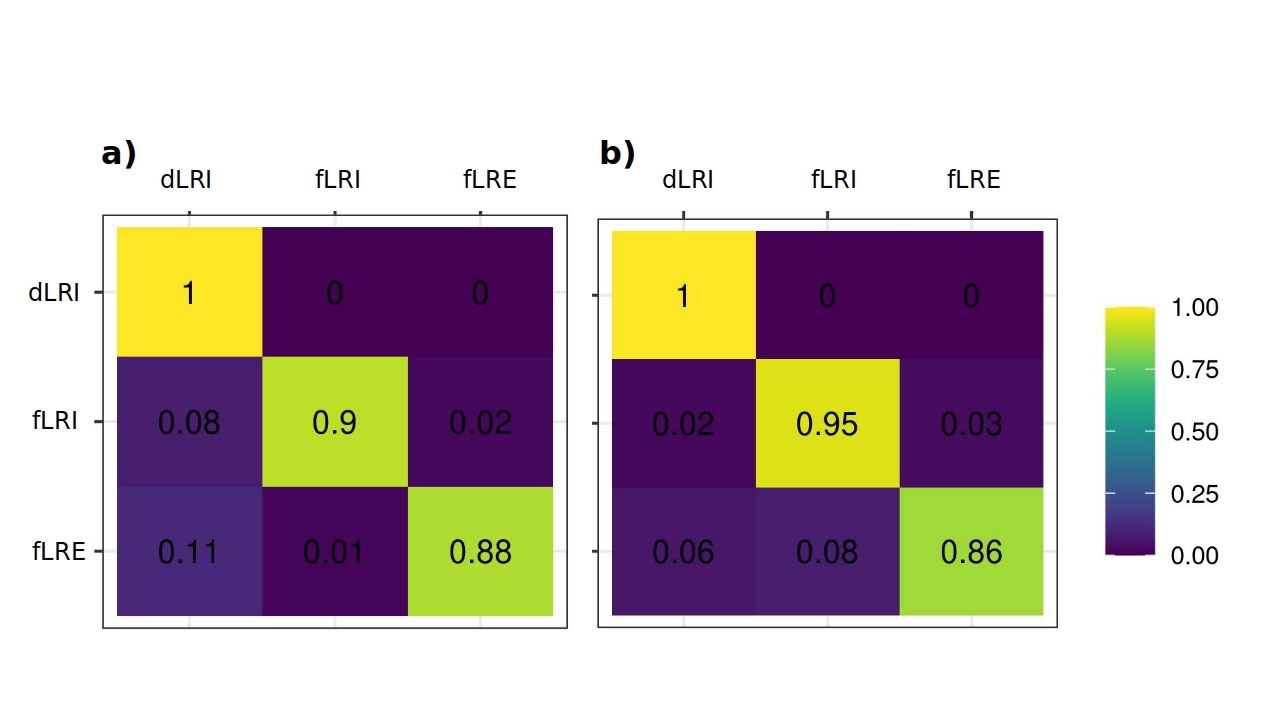
\includegraphics[width=1\textwidth]{figures/ModelRecovery.jpg}}
\caption{\textbf{Model Recovery.} Confusion Matrices showing model recovery for a) experiment 1 and b) experiment 2. The numbers show the probability of data generate by model X to be best fit by model Y.}
\label{fig:model_recovery}
\end{figure}

\subsection*{Simulated and Actual comparison for dLRI and fLRE models}
Figures \ref{fig:simvsemp_dlr_flrI_exp1} and \ref{fig:simvsemp_dlr_flrI_exp2} show a comparison between simulated and actual data for the models instructive model with a decreasing learning rate (dLRI) and the evaluative model with a free learning rate (fLRE).

 

\begin{figure}[ht!]
{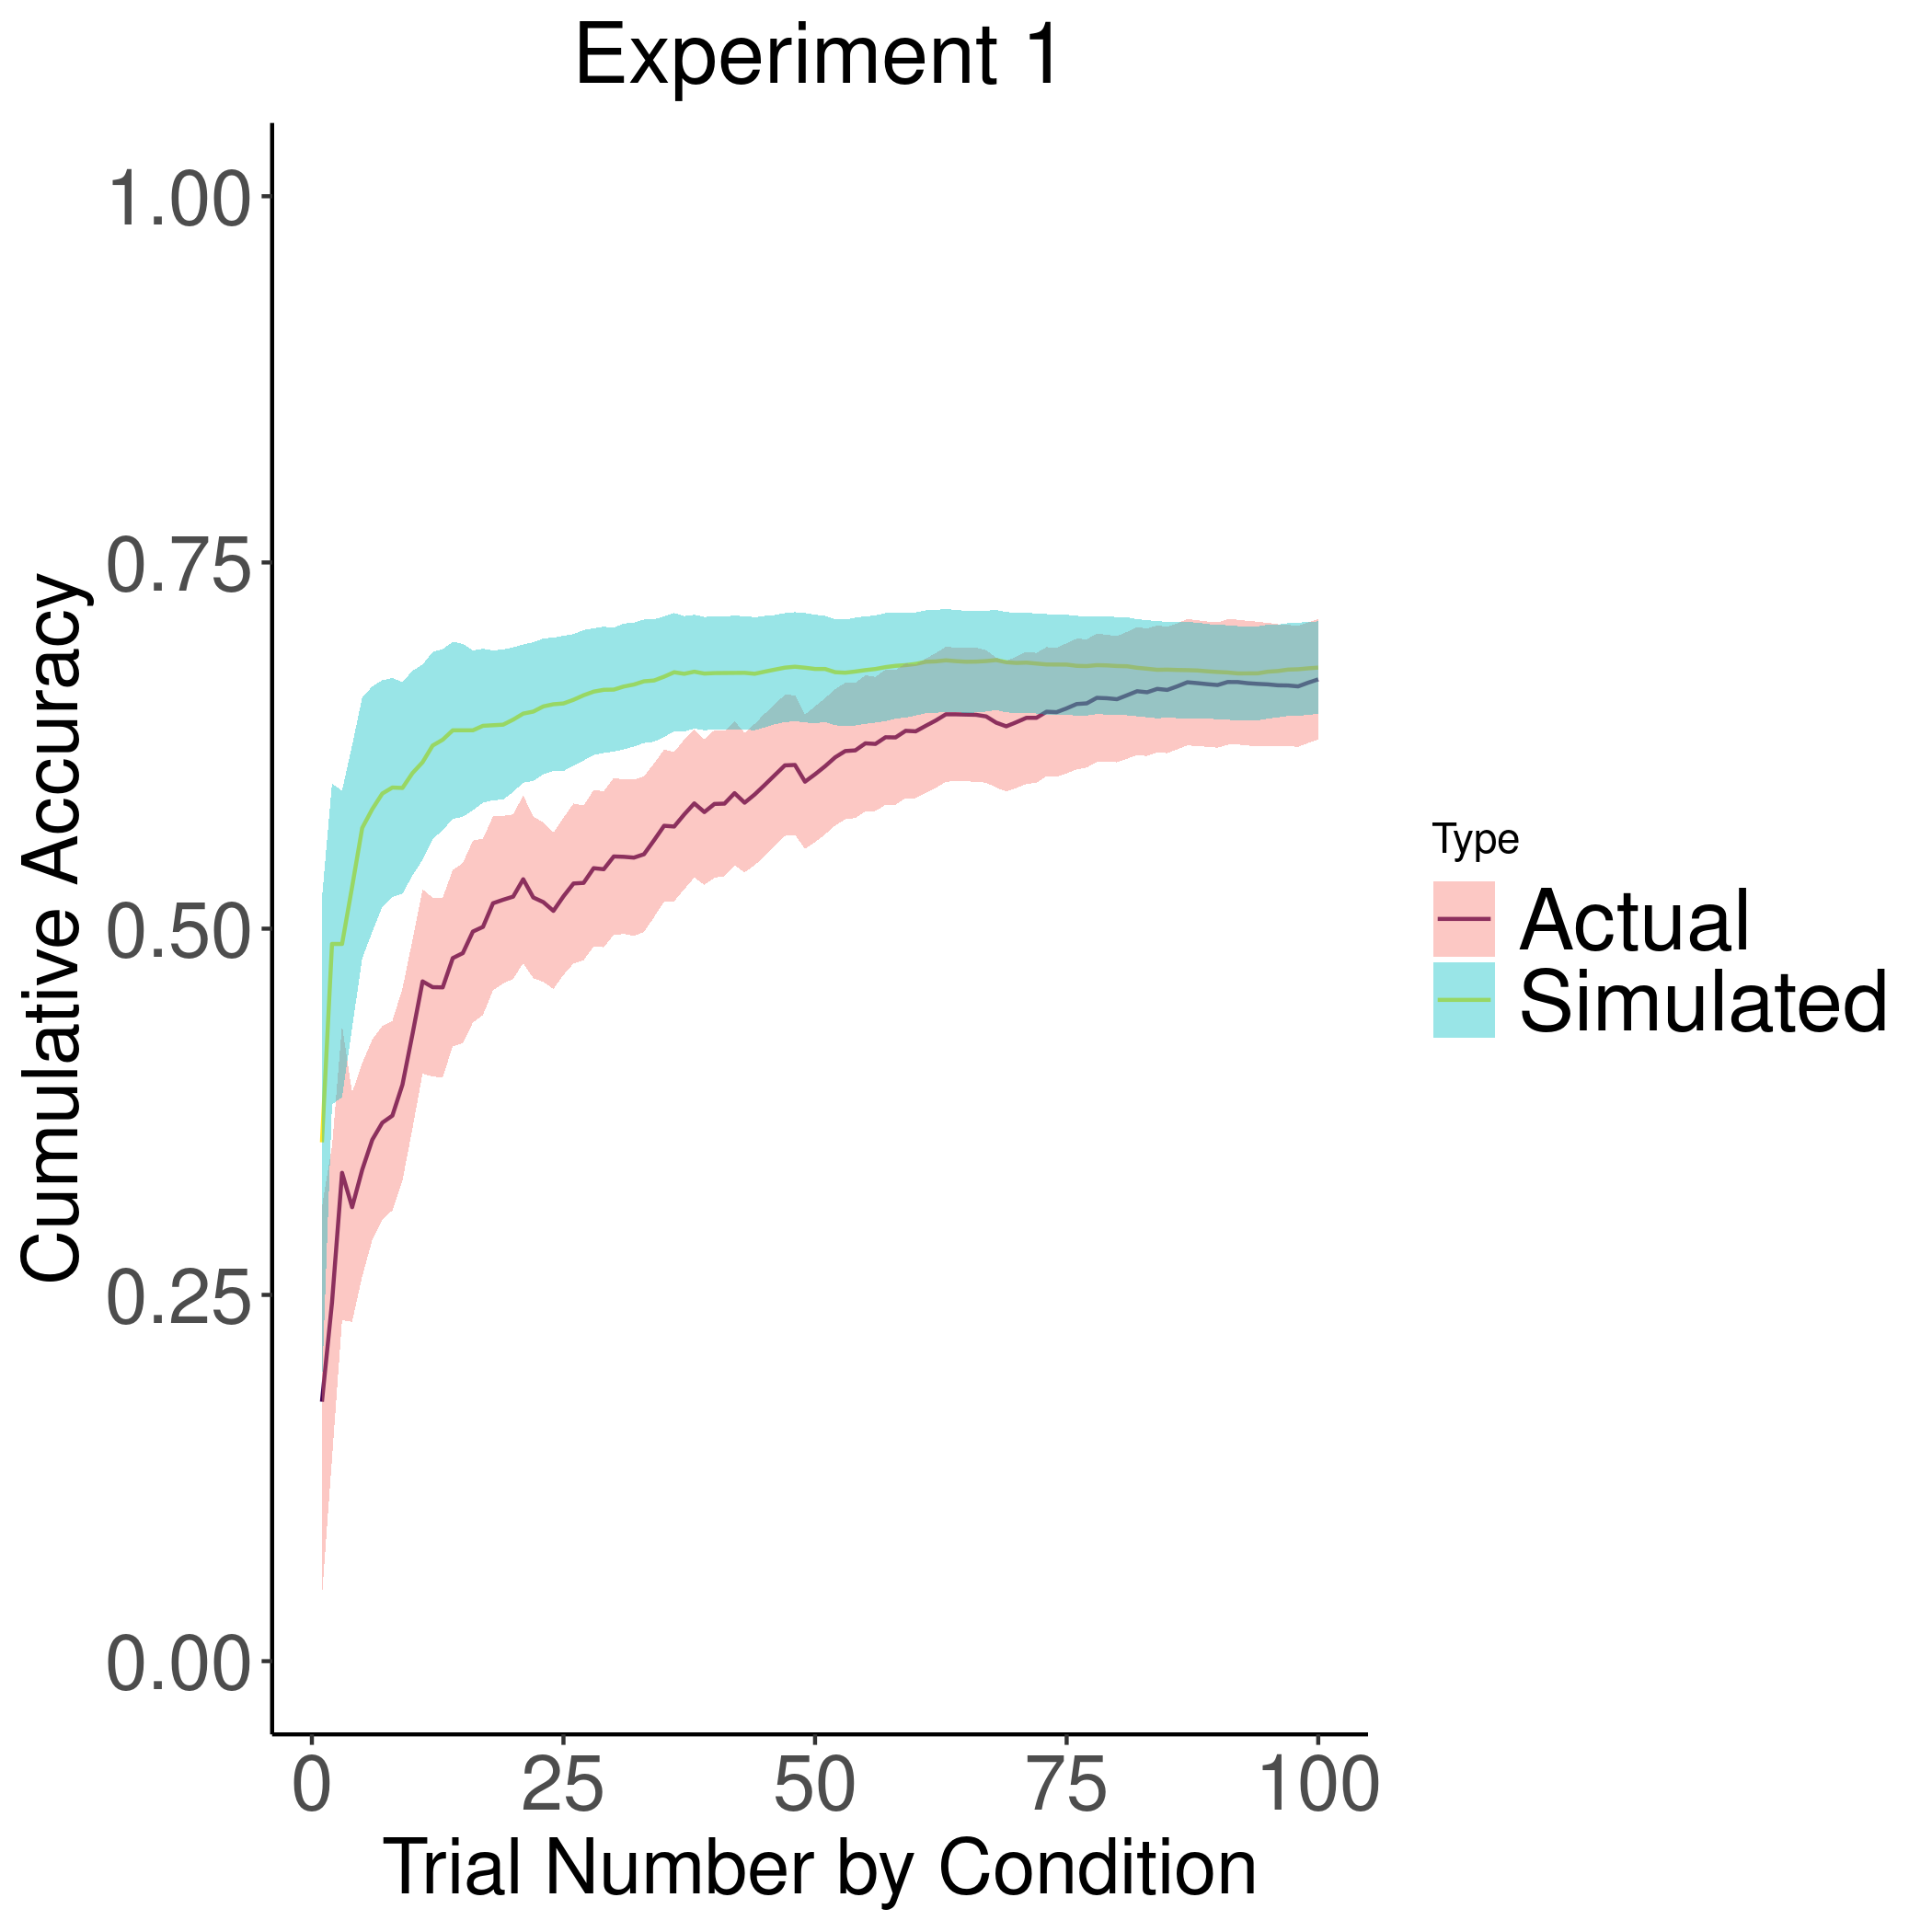
\includegraphics{figures/SimulatedVsActual.exp=exp1.mod=dLR_Instr.png}}\vfill
{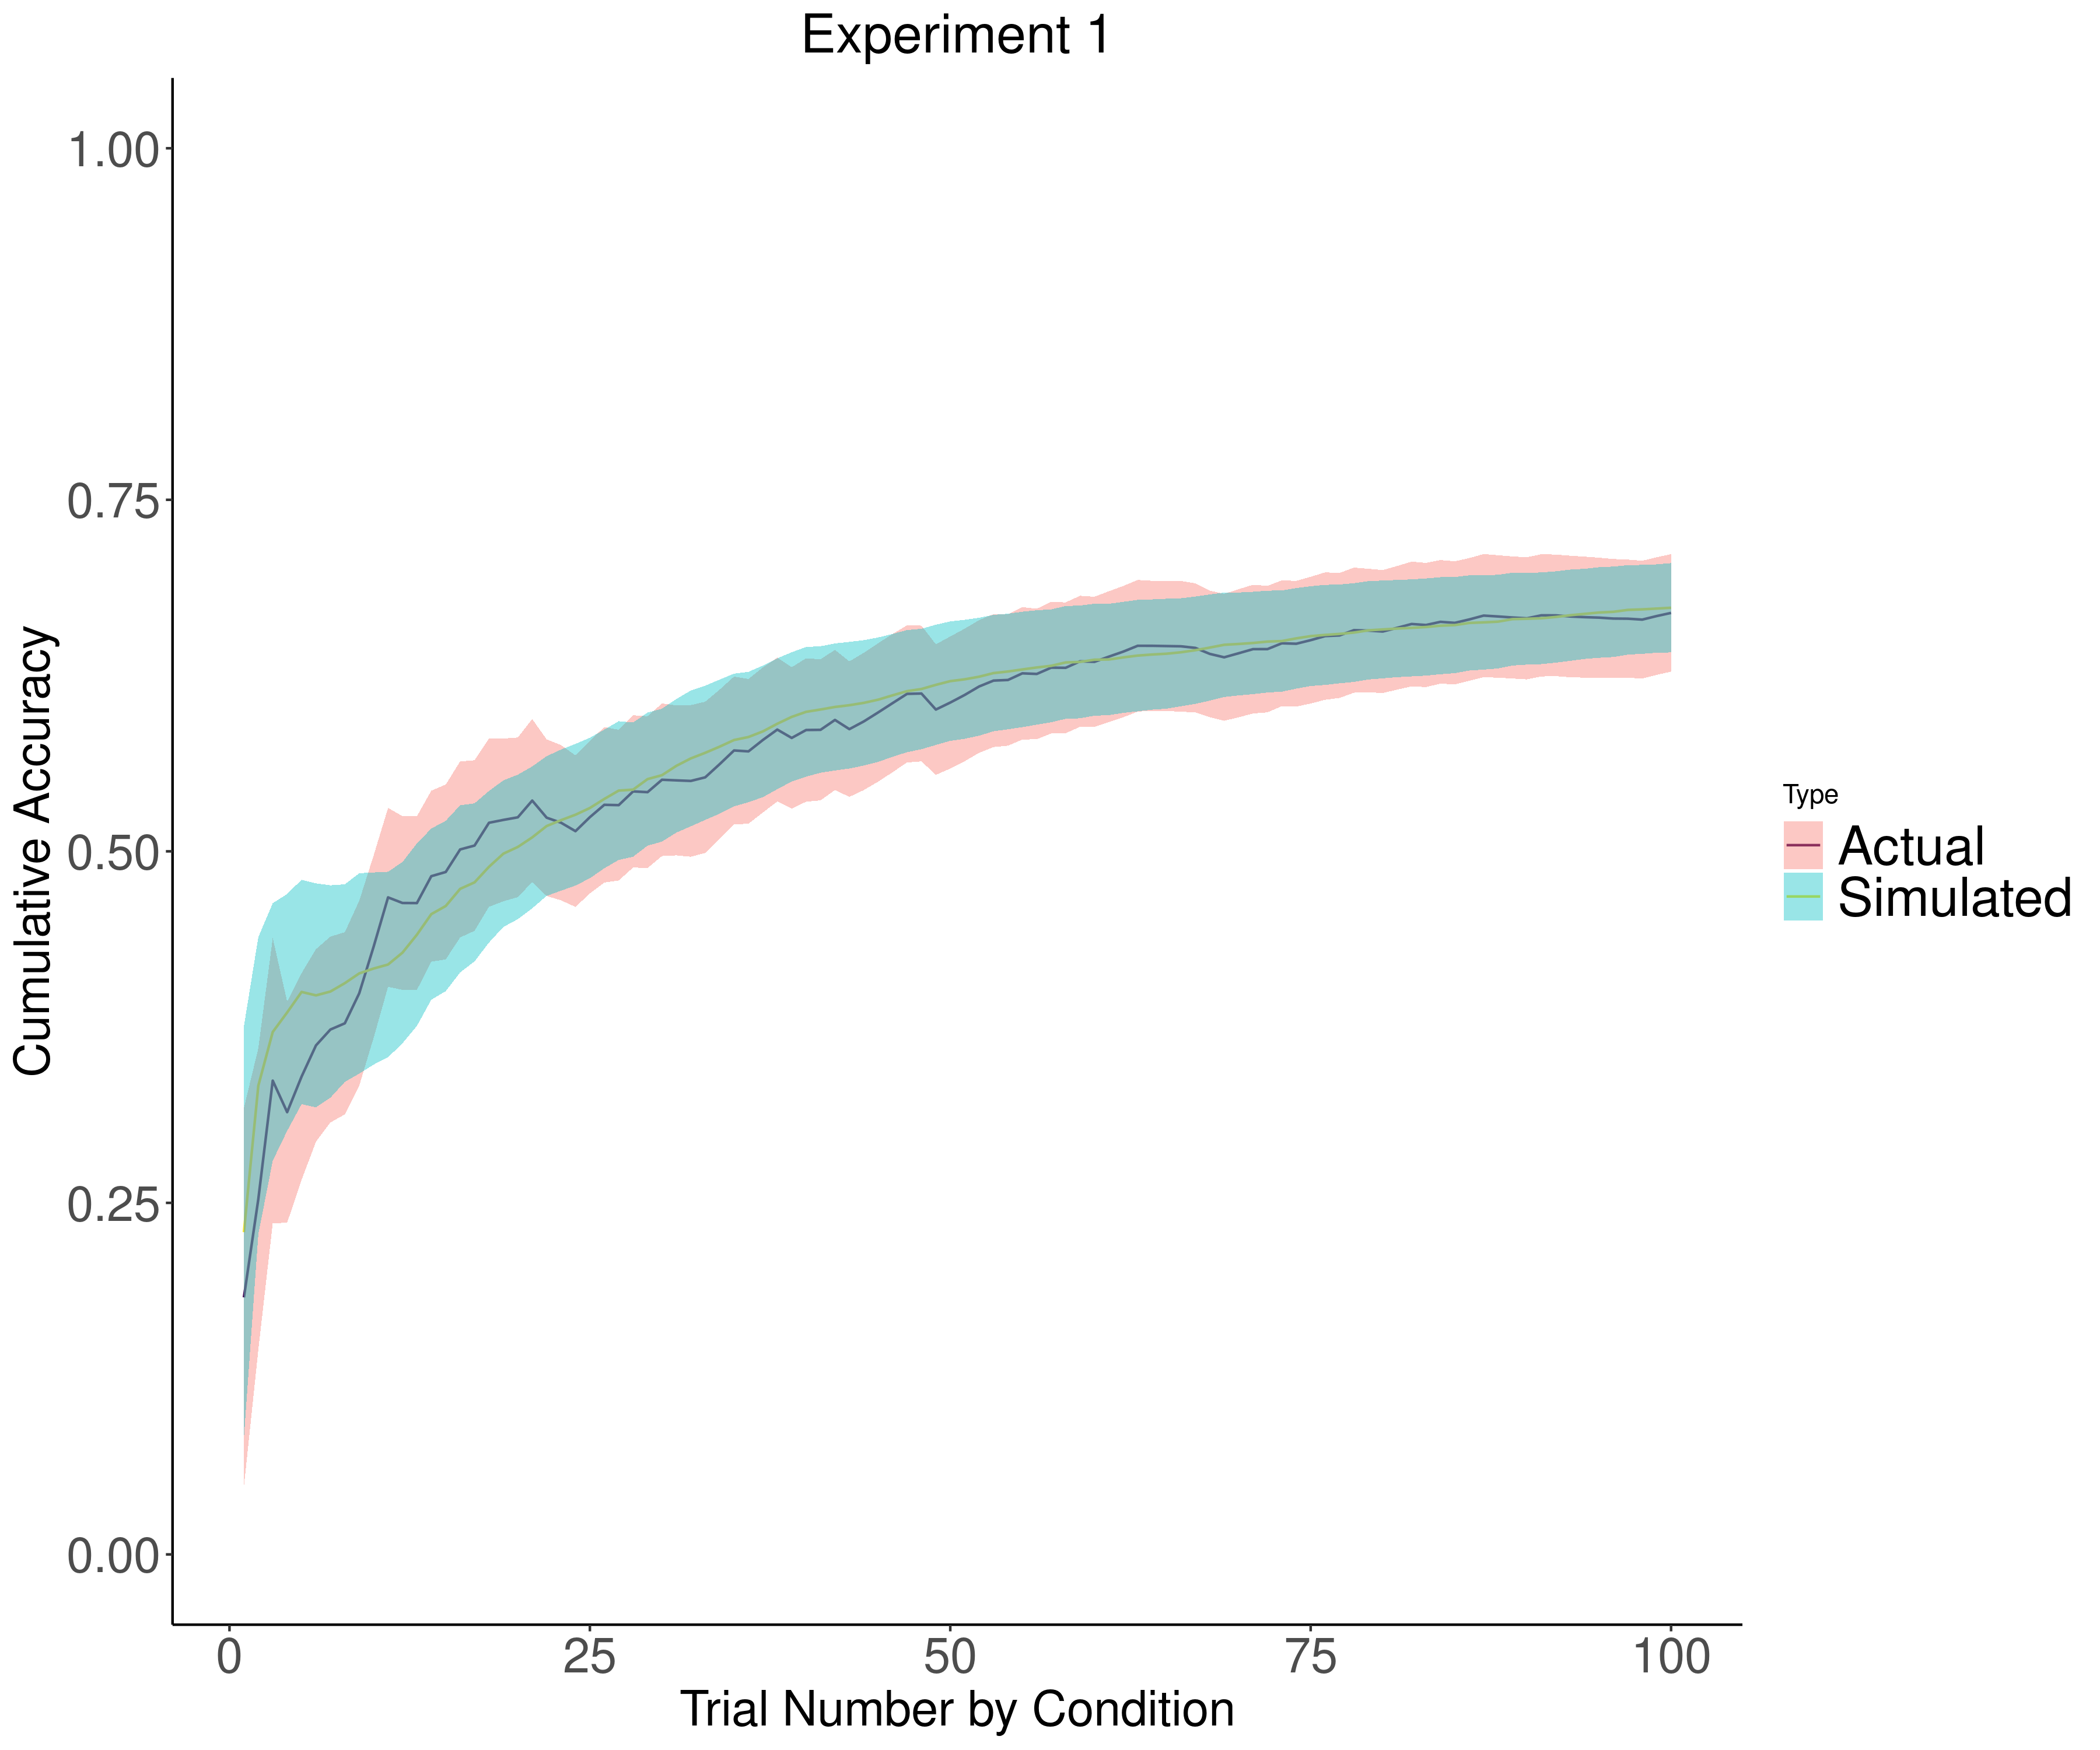
\includegraphics{figures/SimulatedVsActual.exp=exp1.mod=fLR_Eval.png}}
\caption{\textbf{Simulated vs Empirical Data for the Experiment 1 for the dLRI model (left) and fLRE (right).} Simulated data (red line) and actual data (green line) overlapped, for experiment 1, for weak priors condition and strong prior condition. }
\label{fig:simvsemp_dlr_flrI_exp1}
\end{figure}

\begin{figure}[ht!]
{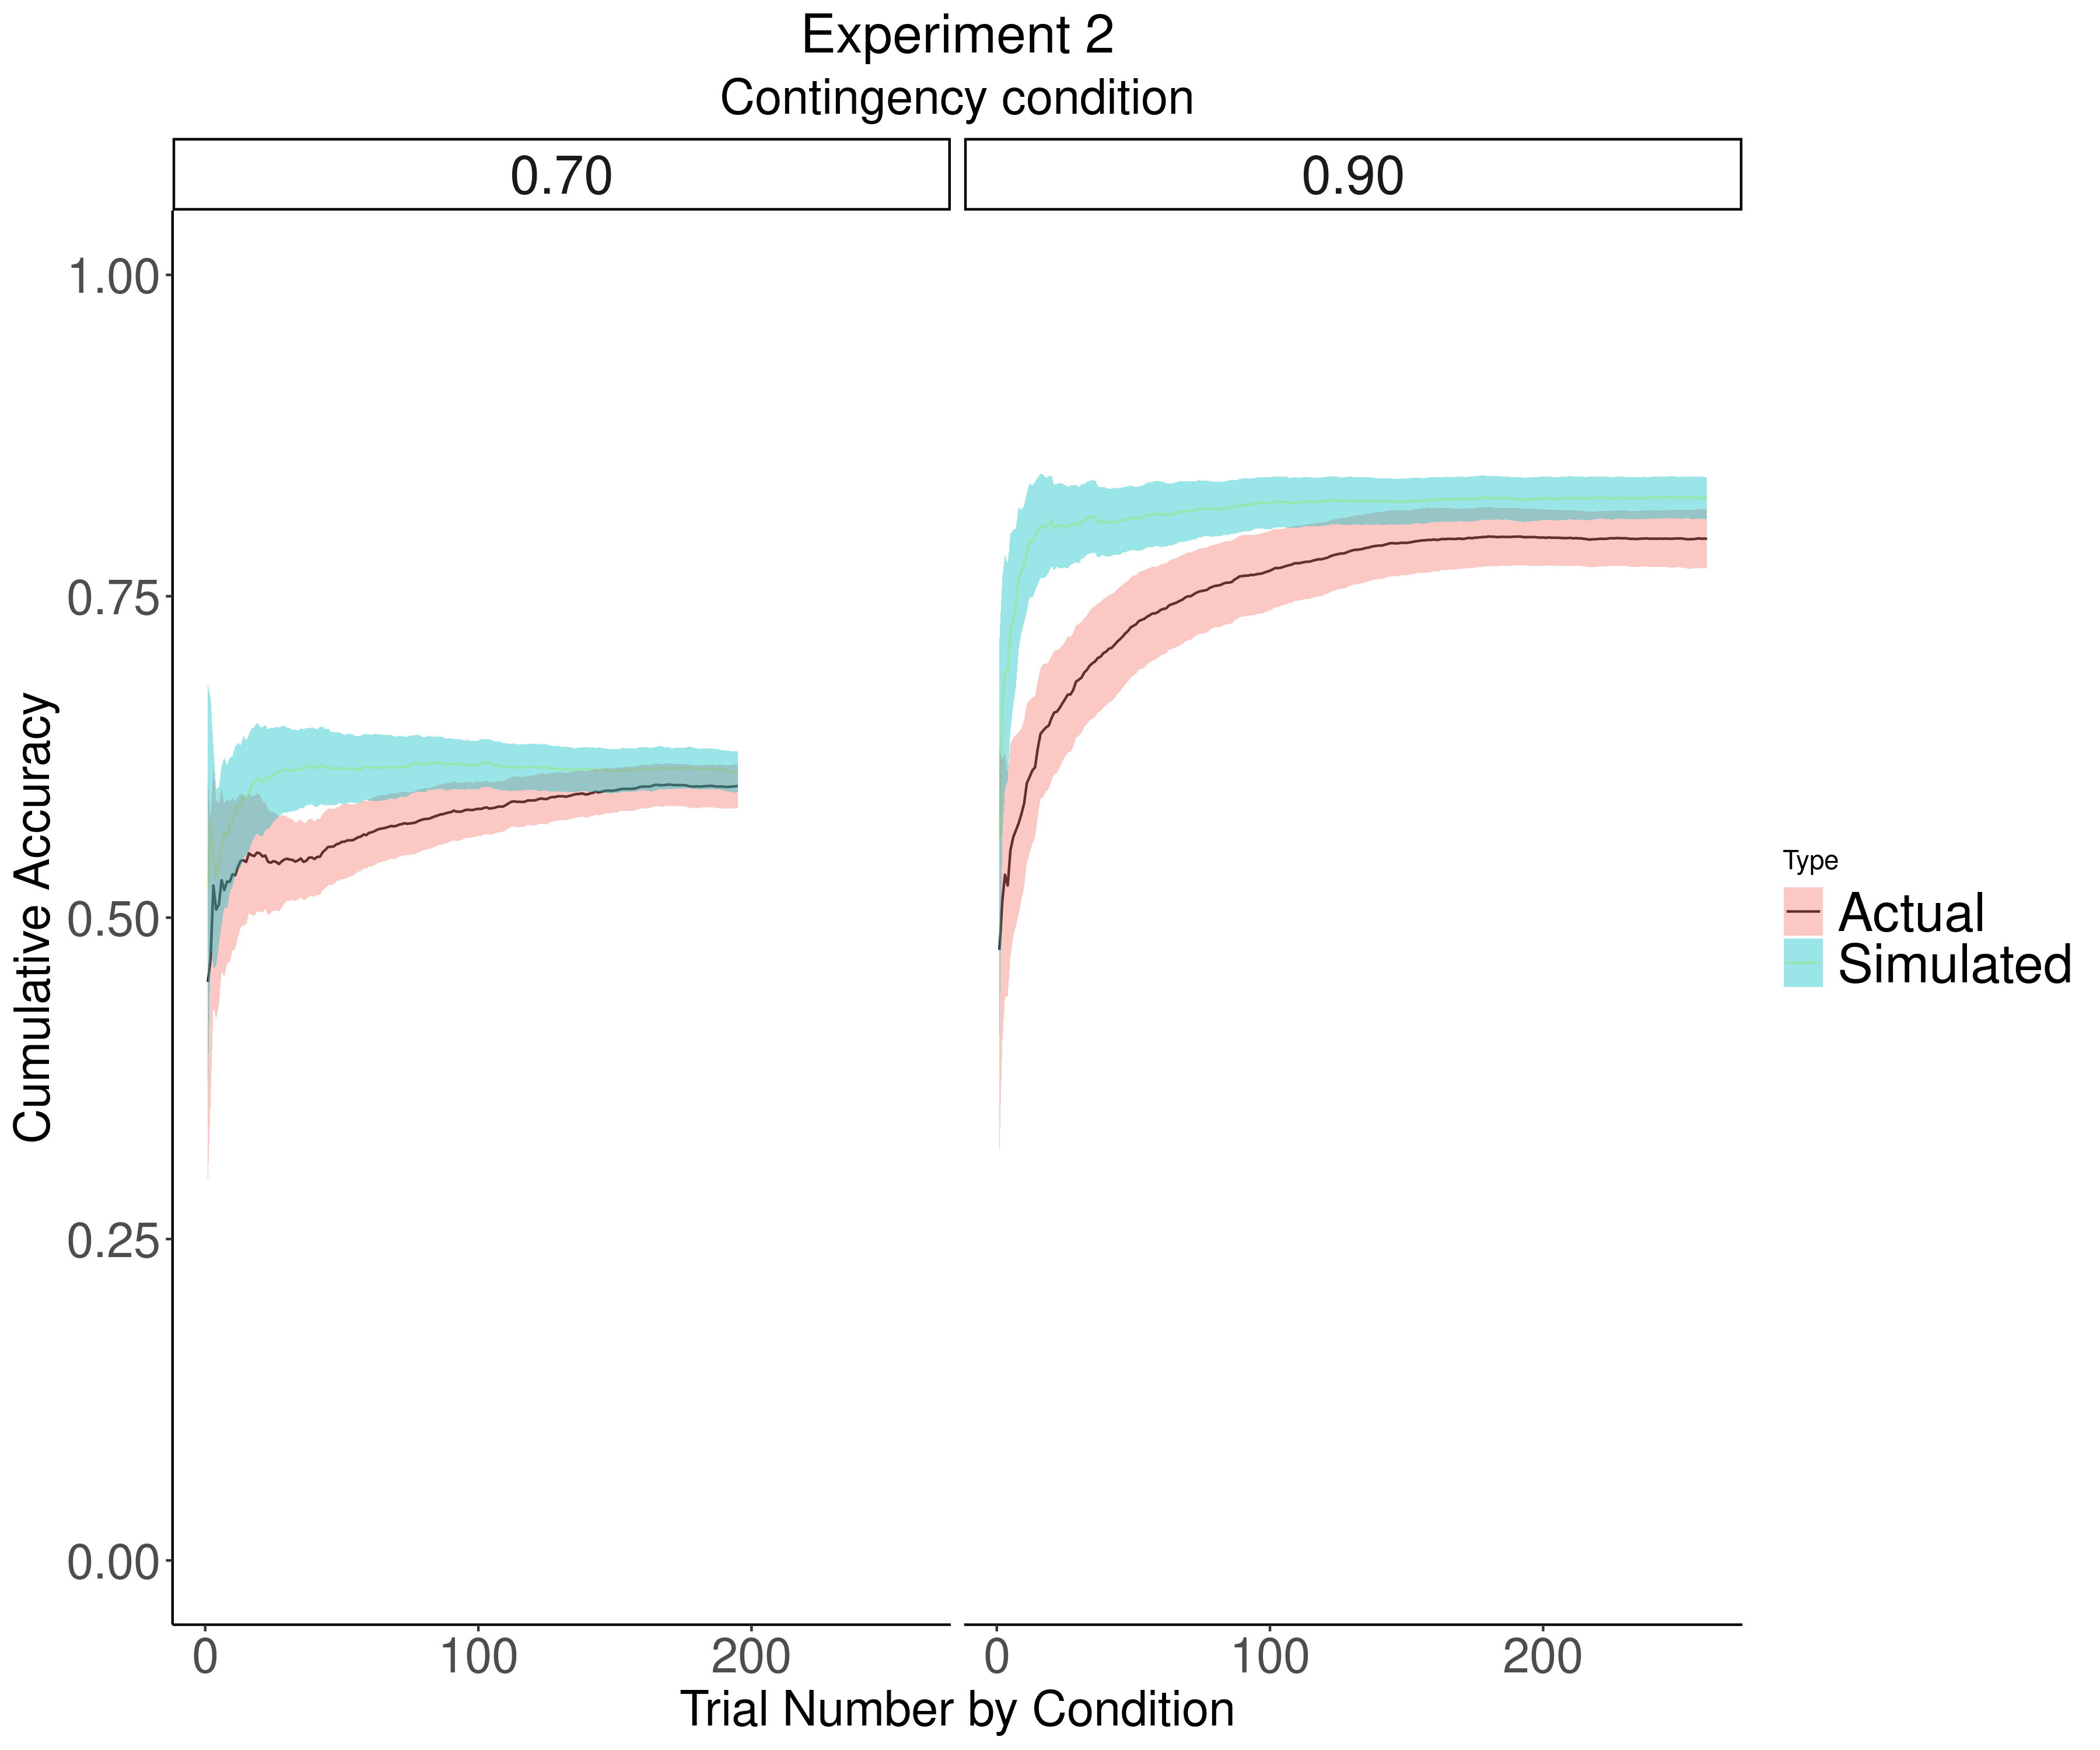
\includegraphics{figures/SimulatedVsActual.exp=exp2.mod=dLR_Instr.png}} \vfill
{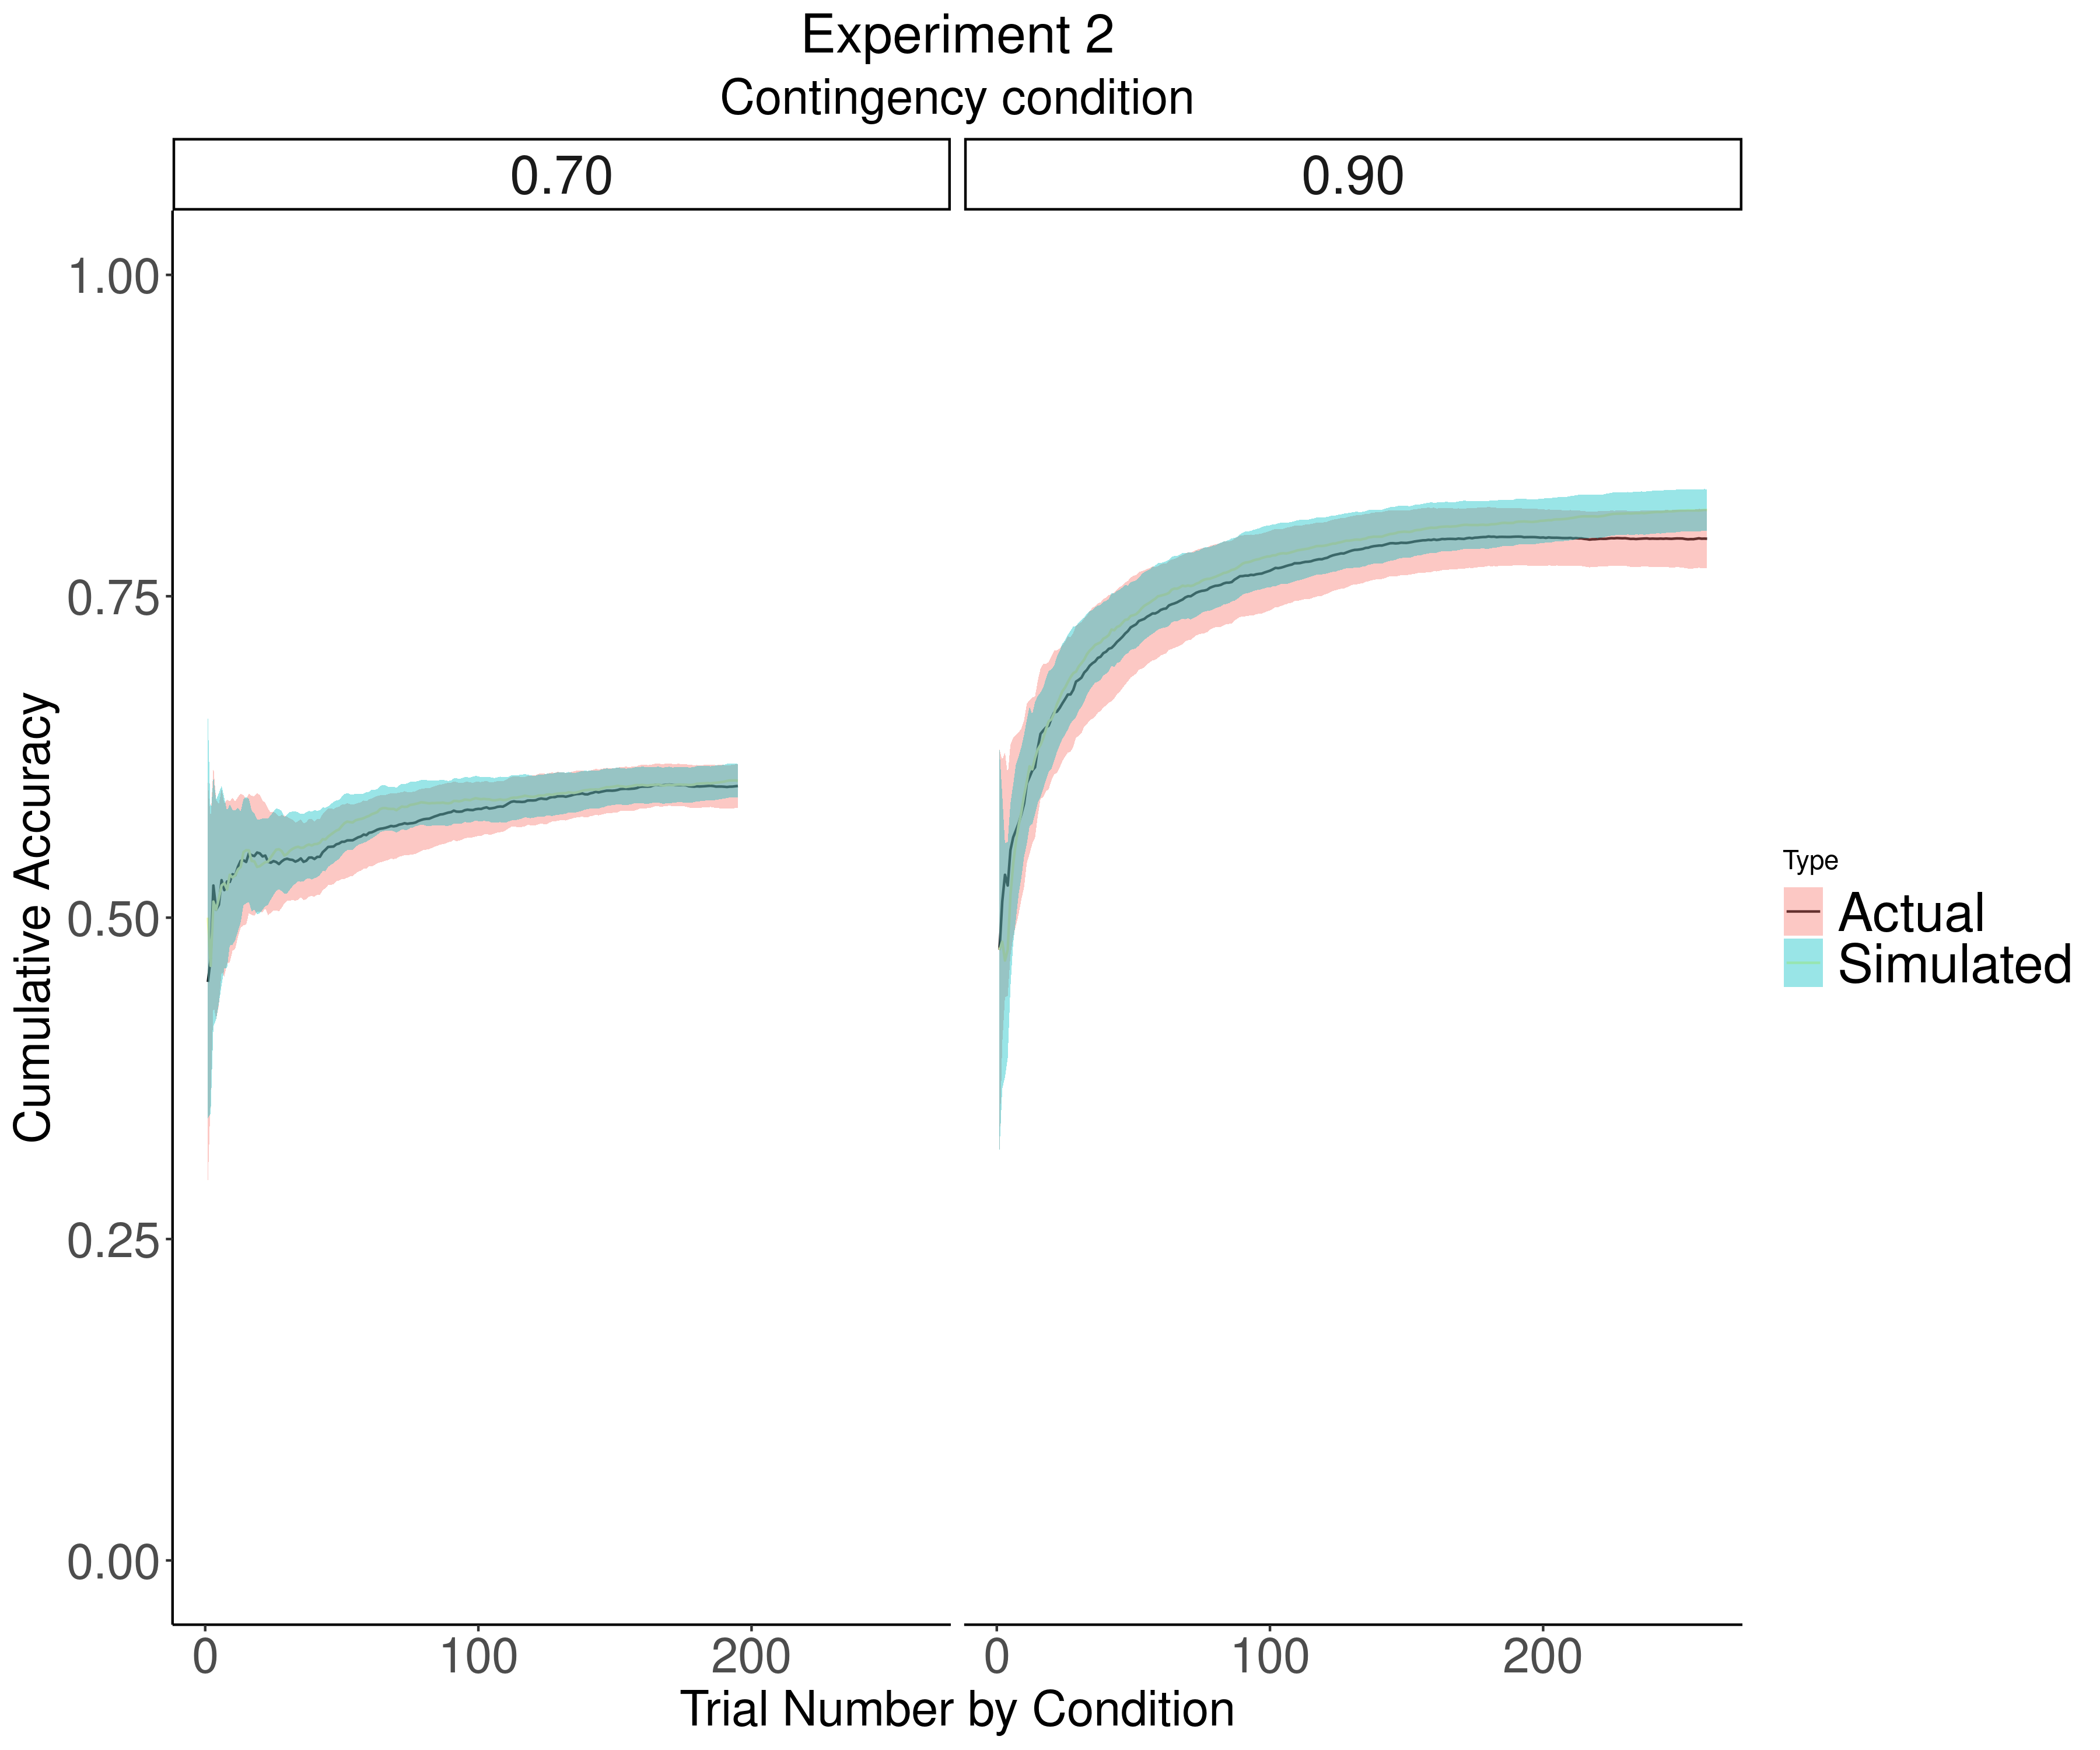
\includegraphics{figures/SimulatedVsActual.exp=exp2.mod=fLR_Eval.png}}
\caption{\textbf{Simulated vs Empirical Data for the Experiment 2 for the dLRI  (left) and fLRE (right).} Simulated data (red line) and actual data (green line) overlapped, for experiment 2, for weak priors condition and strong prior condition. }
\label{fig:simvsemp_dlr_flrI_exp2}
\end{figure}

\subsection*{Analysis with binned Hit Rate}
In order to compare memory at different levels of the model-derived PE, we calculated the quartiles for PE for each participant, separately for trials with correct and incorrect prediction outcome.
We binned the hit rate by aggregating it between the quartiles, to create four bins which eventually were used as the explanatory variable in our analysis. A graph with the distribution of PE by binned data is shown in Figure \ref{fig:PEbin_distr}.

\begin{figure}[ht!]
{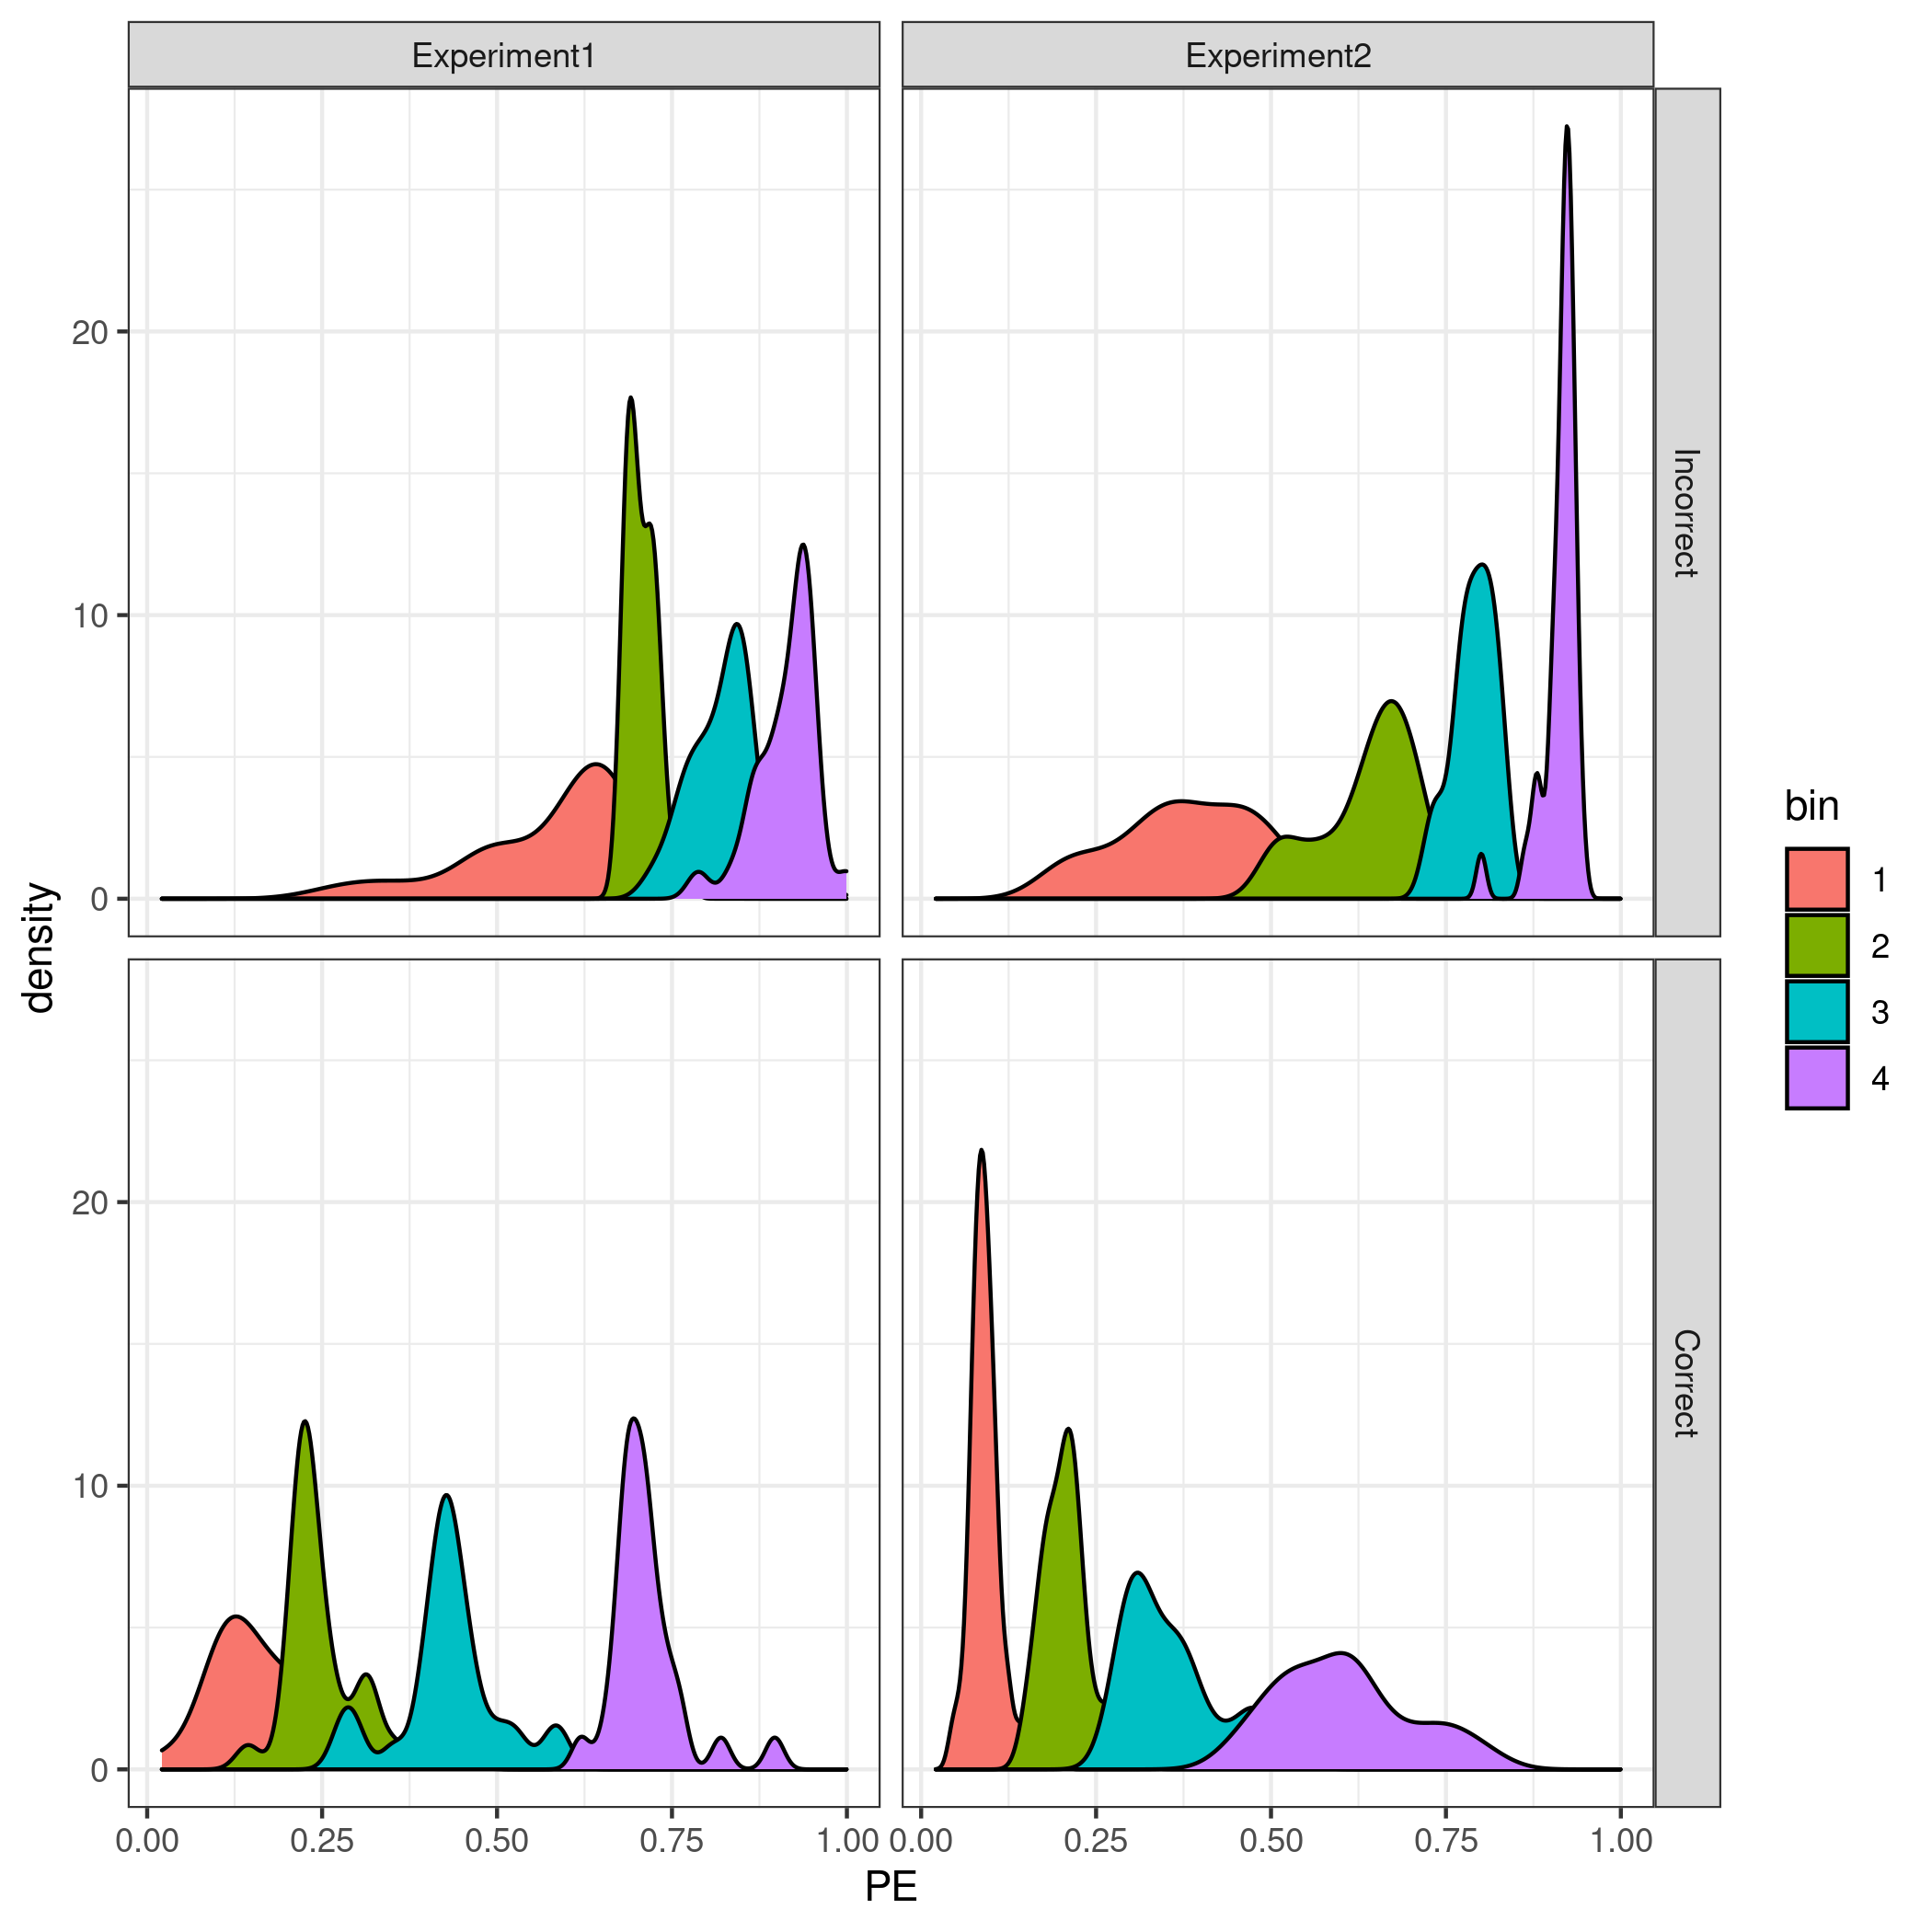
\includegraphics[width=1\textwidth]{figures/PEdistr_binned.png}}
\caption{\textbf{Distribution of binned PE.}Distribution of PE after binning it, as a function of prediction outcome and experiment. }
\label{fig:PEbin_distr}

\end{figure}

\begin{figure}[ht!]
{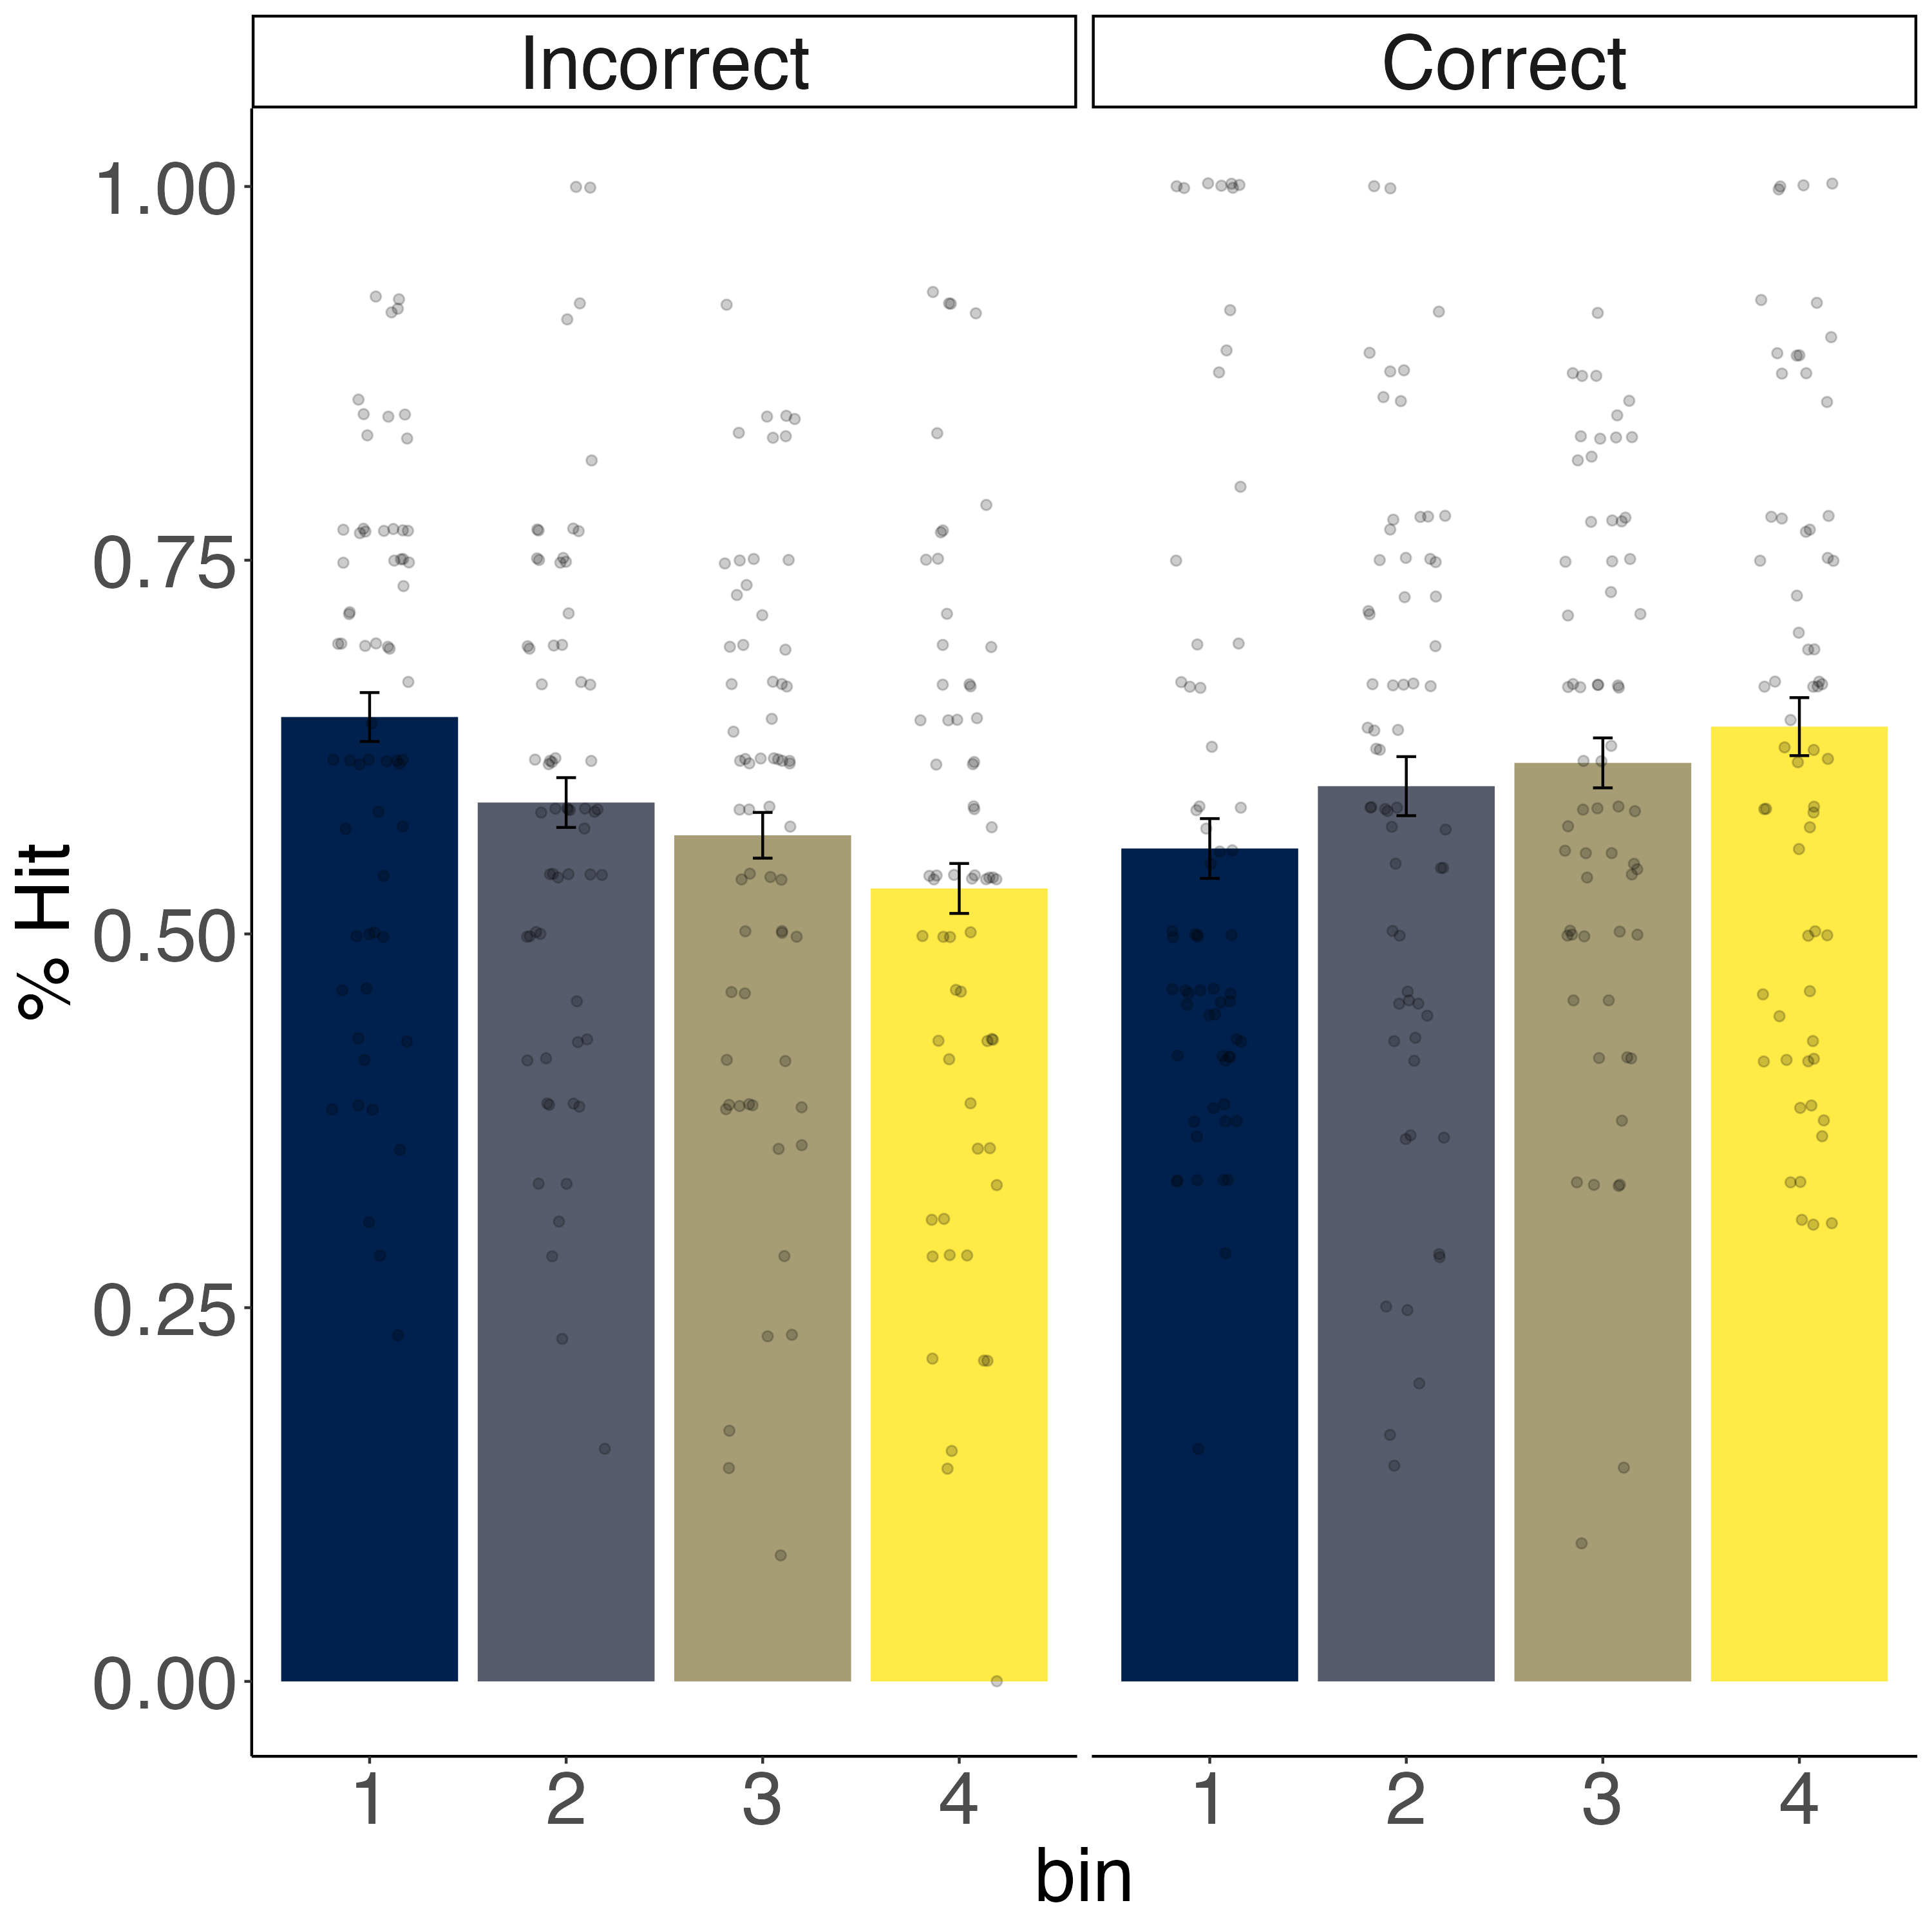
\includegraphics[width=1\textwidth]{figures/binnedPE_mem.png}}
\caption{\textbf{Hit Rate by Binned PE.} Effect of binned PE on hit rate as a function of prediction outcome. }
\label{fig:PEbin_mem}

\end{figure}

Hit rate as a function of binned PE and prediction outcome is shown in Figure \ref{fig:PEbin_mem}. 
 We then tested for the three-way interaction between binned PE, prediction outcome, and experiment, in a linear mixed-effects model, adding participants as random effects. The three-way interaction was not significant, $\chi^2_{(3)}$ = 4.23, \textit{p} = .238. In addition, the interactions between PE and experiment, and the interaction between prediction outcome and experiment were not significant ($\chi^2_{(3)}$ = 1.68, \textit{p} = .642, $\chi^2_{(3)}$ = 0.81, \textit{p} = 0.368, respectively). These results suggest that there were not significant differences in the effects of PE and in the interaction between PE and prediction outcome between the two experiments. By contrast, there was a main effect of experiment, $\chi^2_{(3)}$ = 7.70,  \textit{p} = .005,  showing that overall participants’ performance was significantly worse in Experiment 2, compared to Experiment 1. Importantly, there was also a significant interaction between PE and prediction outcome, $\chi^2_{(3)}$ = 14.09, \textit{p} = .003.\par
 To break down the interaction, the effect of PE on recognition was analyzed separately for correct and incorrect prediction outcomes. We compared each bin with the first one, to test whether increasingly higher PE significantly affected memory encoding. Results showed that for incorrect prediction outcomes, the difference between the first and the second was significant,$\beta$ = - 0.0557, $p_{corr}$ = .040, OR = 1.06. In addition, the comparisons between the third and the first, and the fourth and the first, were both significant, ($p_{corr}$ < .001). For correct prediction outcomes, the comparison between first and second quantile, and first and third quantile did not reach significance ($ps_{corr}$  >.114), whereas the comparison between the fourth and the first quantile was significant,$\beta$ = 0.081, $p_{corr}$ = .009, OR = 1.08. These results suggest that while a PE error generated by incorrect prediction impairs memory even when prior expectations are not very strong, for correct predictions a higher PE is needed in order to observe benefits for memory encoding. 

\end{document}